%
%   $Id$
%   This file is part of the FPC documentation.
%   Copyright (C) 1997, by Michael Van Canneyt
%
%   The FPC documentation is free text; you can redistribute it and/or
%   modify it under the terms of the GNU Library General Public License as
%   published by the Free Software Foundation; either version 2 of the
%   License, or (at your option) any later version.
%
%   The FPC Documentation is distributed in the hope that it will be useful,
%   but WITHOUT ANY WARRANTY; without even the implied warranty of
%   MERCHANTABILITY or FITNESS FOR A PARTICULAR PURPOSE.  See the GNU
%   Library General Public License for more details.
%
%   You should have received a copy of the GNU Library General Public
%   License along with the FPC documentation; see the file COPYING.LIB.  If not,
%   write to the Free Software Foundation, Inc., 59 Temple Place - Suite 330,
%   Boston, MA 02111-1307, USA.
%
%%%%%%%%%%%%%%%%%%%%%%%%%%%%%%%%%%%%%%%%%%%%%%%%%%%%%%%%%%%%%%%%%%%%%%%
% Preamble.
\input{preamble.inc}
\latex{%
  \ifpdf
  \pdfinfo{/Author(Michael Van Canneyt)
           /Title(Programmers' Guide)
           /Subject(Free Pascal Programmers' guide)
           /Keywords(Free Pascal)
           }
  \fi
}
%
% Settings
%
\makeindex
\FPCexampledir{progex}
%
% Start of document.
%
\begin{document}
\title{Free Pascal \\ Programmers' manual}
\docdescription{Programmers' manual for \fpc, version \fpcversion}
\docversion{1.8}
\input{date.inc}
\author{Micha\"el Van Canneyt}
\maketitle
\tableofcontents
\newpage
\listoftables
\newpage

%%%%%%%%%%%%%%%%%%%%%%%%%%%%%%%%%%%%%%%%%%%%%%%%%%%%%%%%%%%%%%%%%%%%%
% Introduction
%%%%%%%%%%%%%%%%%%%%%%%%%%%%%%%%%%%%%%%%%%%%%%%%%%%%%%%%%%%%%%%%%%%%%
\section*{About this document}
This is the programmer's manual for \fpc.

It describes some of the peculiarities of the \fpc compiler, and provides a
glimpse of how the compiler generates its code, and how you can change the
generated code. It will not, however, provide a detailed account of
the inner workings of the compiler, nor will it describe how to use the
compiler (described in the \userref). It also will not describe the inner
workings of the Run-Time Library (RTL). The best way to learn about the way
the RTL is implemented is from the sources themselves.

The things described here are useful when things need to be done that
require greater flexibility than the standard Pascal language constructs
(described in the \refref).

Since the compiler is continuously under development, this document may get
out of date. Wherever possible, the information in this manual will be
updated. If you find something which isn't correct, or you think something
 is missing, feel free to contact me\footnote{at
\var{Michael.VanCanneyt@wisa.be}}.

%%%%%%%%%%%%%%%%%%%%%%%%%%%%%%%%%%%%%%%%%%%%%%%%%%%%%%%%%%%%%%%%%%%%%
% Compiler switches
%%%%%%%%%%%%%%%%%%%%%%%%%%%%%%%%%%%%%%%%%%%%%%%%%%%%%%%%%%%%%%%%%%%%%
\chapter{Compiler directives}
\label{ch:CompSwitch}

\fpc supports compiler directives in the source file. They are not the same
as Turbo Pascal directives, although some are supported for compatibility.
There is a distinction between local and global directives; local directives
take effect from the moment they are encountered, global directives have an
effect on all of the compiled code.

Many switches have a long form also. If they do, then the name of the
long form is given also. For long switches, the + or - character to switch
the option on or off, may be replaced by \var{ON} or \var{OFF} keywords.

Thus \verb|{$I+}| is equivalent to \verb|{$IOCHECKS ON}| or
\verb|{$IOCHECKS +}| and
\verb|{$C-}| is equivalent to \verb|{$ASSERTIONS OFF}| or
\verb|{$ASSERTIONS -}|

The long forms of the switches are the same as their Delphi
counterparts.

%%%%%%%%%%%%%%%%%%%%%%%%%%%%%%%%%%%%%%%%%%%%%%%%%%%%%%%%%%%%%%%%%%%%%
% Local switches
\section{Local directives}
\label{se:LocalSwitch}
Local directives can occur more than once in a unit or program,
If they have a command-line counterpart, the command-line argument is
restored as the default for each compiled file. The local directives
influence the compiler's behaviour from the moment they're encountered
until the moment another switch annihilates their behaviour, or the end
of the current unit or program is reached.

\subsection{\var{\$A} or \var{\$ALIGN} : Align Data}

This switch is recognized for Turbo Pascal Compatibility, but is not
yet implemented. The alignment of data will be different in any case.

\subsection{\var{\$ASMMODE} : Assembler mode (Intel 80x86 only)}
\label{se:AsmReader}

The \var{\{\$ASMMODE XXX\}} directive informs the compiler what kind of assembler
it can expect in an \var{asm} block. The \var{XXX} should be replaced by one
of the following:
\begin{description}
\item [att\ ] Indicates that \var{asm} blocks contain AT\&T syntax assembler.
\item [intel\ ] Indicates that \var{asm} blocks contain Intel syntax
assembler.
\item [direct\ ] Tells the compiler that asm blocks should be copied
directly to the assembler file.
\end{description}
These switches are local, and retain their value to the end of the unit that
is compiled, unless they are replaced by another directive of the same type.
The command-line switch that corresponds to this switch is \var{-R}.

The default assembler reader is the AT\&T reader.

\subsection{\var{\$B} or \var{\$BOOLEVAL} : Complete boolean evaluation}

This switch is understood by the \fpc compiler, but is ignored. The compiler
always uses shortcut evaluation, i.e. the evaluation of a boolean expression
is stopped once the result of the total exression is known with certainty.

So, in the following example, the function \var{Bofu}, which has a boolean
result, will never get called.
\begin{verbatim}
If False and Bofu then
  ...
\end{verbatim}
This has as a consequence that any additional actions that are done by
\var{Bofu} are not executed.

\subsection{\var{\$C} or \var{\$ASSERTIONS} : Assertion support}

The \var{\{\$ASSERTION\}} switch determines if assert statements are
compiled into the binary or not. If the switch is on, the statement
\begin{verbatim}
Assert(BooleanExpression,AssertMessage);
\end{verbatim}
Will be compiled in the binary. If te \var{BooleanExpression} evaluates to
\var{False}, the RTL will check if the \var{AssertErrorProc} is set. If it
is set, it will be called with as parameters the \var{AssertMessage}
message, the name of the file, the LineNumber and the address. If it is not
set, a runtime error 227 is generated.

The \var{AssertErrorProc} is defined as
\begin{verbatim}
Type
  TAssertErrorProc=procedure(const msg,fname:string;lineno,erroraddr:longint);
Var
  AssertErrorProc = TAssertErrorProc;
\end{verbatim}
This can be used mainly for debugging purposes. The \file{system} unit sets the
\var{AssertErrorProc} to a handler that displays a message on \var{stderr}
and simply exits. The \file{sysutils} unit catches the run-time error 227
and raises an \var{EAssertionFailed} exception.

\subsection{\var{\$DEFINE} : Define a symbol}

The directive
\begin{verbatim}
{$DEFINE name}
\end{verbatim}
defines the symbol \var{name}. This symbol remains defined until the end of
the current module (i.e. unit or program), or until a \var{\$UNDEF name} directive is encountered.

If \var{name} is already defined, this has no effect. \var{Name} is case
insensitive.

The symbols that are defined in a unit, are not saved in the unit file,
so they are also not exported from a unit.

\subsection{\var{\$ELSE} : Switch conditional compilation}

The \var{\{\$ELSE\}} switches between compiling and ignoring the source
text delimited by the preceding \var{\{\$IFxxx\}} and following
\var{\{\$ENDIF\}}. Any text after the \var{ELSE} keyword but before the
brace is ignored:
\begin{verbatim}
{$ELSE some ignored text}
\end{verbatim}
is the same as
\begin{verbatim}
{$ELSE}
\end{verbatim}
This is useful for indication what switch is meant.

\subsection{\var{\$ENDIF} : End conditional compilation}

The \var{\{\$ENDIF\}} directive ends the conditional compilation initiated by the
last \var{\{\$IFxxx\}} directive. Any text after the \var{ENDIF} keyword but
before the closing brace is ignored:
\begin{verbatim}
{$ENDIF some ignored text}
\end{verbatim}
is the same as
\begin{verbatim}
{$ENDIF}
\end{verbatim}
This is useful for indication what switch is meant to be ended.

\subsection{\var{\$ERROR} : Generate error message}

The following code
\begin{verbatim}
{$ERROR This code is erroneous !}
\end{verbatim}
will display an error message when the compiler encounters it,
and increase the error count of the compiler.
The compiler will continue to compile, but no code will be emitted.

\subsection{\var{\$F} : Far or near functions}
This directive is recognized for compatibility with Turbo Pascal. Under the
32-bit and 64-bit programming models, the concept of near and far calls have
no meaning, hence the directive is ignored. A warning is printed to the screen, 
as a reminder.

As an example, the following piece of code:
\begin{verbatim}
{$F+}

Procedure TestProc;

begin
 Writeln ('Hello From TestProc');
end;

begin
 testProc
end.
\end{verbatim}
Generates the following compiler output:
\begin{verbatim}
malpertuus: >pp -vw testf
Compiler: ppc386
Units are searched in: /home/michael;/usr/bin/;/usr/lib/ppc/0.9.1/linuxunits
Target OS: Linux
Compiling testf.pp
testf.pp(1) Warning: illegal compiler switch
7739 kB free
Calling assembler...
Assembled...
Calling linker...
12 lines compiled,
 1.00000000000000E+0000
\end{verbatim}
One can see that the verbosity level was set to display warnings.

When declaring a function as \var{Far} (this has the same effect as setting it
between \var{\{\$F+\} \dots \{\$F-\}} directives), the compiler also generates a
warning:
\begin{verbatim}
testf.pp(3) Warning: FAR ignored
\end{verbatim}

The same story is true for procedures declared as \var{Near}. The warning
displayed in that case is:
\begin{verbatim}
testf.pp(3) Warning: NEAR ignored
\end{verbatim}

\subsection{\var{\$FATAL} : Generate fatal error message}

The following code
\begin{verbatim}
{$FATAL This code is erroneous !}
\end{verbatim}
will display an error message when the compiler encounters it,
and the compiler will immediatly stop the compilation process.

This is mainly useful inc conjunction wih \var{\{\$IFDEF\}} or
\var{\{\$IFOPT\}} statements.

\subsection{\var{\$GOTO} : Support \var{Goto} and \var{Label}}

If \var{\{\$GOTO ON\}} is specified, the compiler will support \var{Goto}
statements and \var{Label} declarations. By default, \var{\$GOTO OFF} is
assumed. This directive corresponds to the \var{-Sg} command-line option.

As an example, the following code can be compiled:
\begin{verbatim}
{$GOTO ON}

label Theend;

begin
  If ParamCount=0 then
    GoTo TheEnd;
  Writeln ('You specified command-line options');
TheEnd:
end.
\end{verbatim}

\begin{remark}When compiling assembler code using the inline assembler
readers, any labels used in the assembler code must be declared, and 
the \var{\{\$GOTO ON\}} directive should be used.
\end{remark}

\subsection{\var{\$H} or \var{\$LONGSTRINGS} : Use AnsiStrings}

If \var{\{\$LONGSTRINGS ON\}} is specified, the keyword \var{String} (no
length specifier) will be treated as \var{AnsiString}, and the compiler
will treat the corresponding variable as an ansistring, and will
generate corresponding code.

By default, the use of ansistrings is off, corresponding to \var{\{\$H-\}}.
The \file{system} unit is compiled without ansistrings, all its functions accept
shortstring arguments. The same is true for all RTL units, except the
\file{sysutils} unit, which is compiled with ansistrings.

\subsection{\var{\$HINT} : Generate hint message}

If the generation of hints is turned on, through the \var{-vh} command-line
option or the \var{\{\$HINTS ON\}} directive, then
\begin{verbatim}
{$Hint This code should be optimized }
\end{verbatim}
will display a hint message when the compiler encounters it.

By default, no hints are generated.

\subsection{\var{\$HINTS} : Emit hints}

\var{\{\$HINTS ON\}} switches the generation of hints on.
\var{\{\$HINTS OFF\}} switches the generation of hints off.
Contrary to the command-line option \var{-vh} this is a local switch,
this is useful for checking parts of the code.

\subsection{\var{\$IF} : Start conditional compilation}

The directive \var{\{\$IF expr\}} will continue the compilation
if the boolean expression \var{expr} evaluates to \var{true}. If the
compilation evaluates to false, then the source is skipped to the first
\var{\{\$ELSE\}} or \var{\{\$ENDIF\}} directive.

The compiler must be able to evaluate the expression at parse time.
This means that variables or constants that are defined in
the source cannot be used. Macros and symbols may be used, however.

More information on this can be found in the section about
conditionals.

\subsection{\var{\$IFDEF Name} : Start conditional compilation}

If the symbol \var{Name} is not defined then the \var{\{\$IFDEF name\}}
will skip the compilation of the text that follows it to the first
\var{\{\$ELSE\}} or \var{\{\$ENDIF\}} directive.
If \var{Name} is defined, then compilation continues as if the directive
wasn't there.

\subsection{\var{\$IFNDEF} : Start conditional compilation}

If the symbol \var{Name} is defined then the \var{\{\$IFNDEF name\}}
will skip the compilation of the text that follows it to the first
\var{\{\$ELSE\}} or \var{\{\$ENDIF\}} directive.
If it is not defined, then compilation continues as if the directive
wasn't there.

\subsection{\var{\$IFOPT} : Start conditional compilation}

The \var{\{\$IFOPT switch\}} will compile the text that follows it if the
switch \var{switch} is currently in the specified state.
If it isn't in the specified state, then compilation continues after the
corresponding \var{\{\$ELSE\}} or \var{\{\$ENDIF\}} directive.

As an example:
\begin{verbatim}
{$IFOPT M+}
  Writeln ('Compiled with type information');
{$ENDIF}
\end{verbatim}
Will compile the writeln statement if generation of type information is on.

\begin{remark}The \var{\{\$IFOPT\}} directive accepts only short options,
i.e. \var{\{\$IFOPT TYPEINFO\}} will not be accepted.
\end{remark}

\subsection{\var{\$INFO} : Generate info message}

If the generation of info is turned on, through the \var{-vi} command-line
option, then
\begin{verbatim}
{$INFO This was coded on a rainy day by Bugs Bunny}
\end{verbatim}
will display an info message when the compiler encounters it.

This is useful in conjunction with the \var{\{\$IFDEF\}} directive, to show
information about which part of the code is being compiled.

\subsection{\var{\$INLINE} : Allow inline code.}

The \var{\{\$INLINE ON\}} directive tells the compiler that the \var{Inline}
procedure modifier should be allowed. Procedures that are declared inline
are copied to the places where they are called. This has the effect that
there is no actual procedure call, the code of the procedure is just copied
to where the procedure is needed, this results in faster execution speed if
the function or procedure is used a lot.

By default, \var{Inline} procedures are not allowed. This directive must be 
specified to use inlined code. The directive is equivalent to the command-line
 switch \var{-Si}. For more information on inline routines, consult the \refref.

\subsection{\var{\$I} or \var{\$IOCHECKS} : Input/Output checking}

The \var{\{\$I-\}} or \var{\{\$IOCHECKS OFF\}} directive tells the compiler
not to generate input/output checking code in the program. By default, the
compiler does not generate this code, it must be switched on using the \var{-Ci}
command-line switch.

When compiling using the \var{-Ci} compiler switch, the \fpc compiler inserts
input/output checking code after every input/output call in the code.
If an error occurred during input or output, then a run-time error will
be generated. Use this switch to avoid this behaviour.

To check if something went wrong, the \var{IOResult} function can be used
to see if everything went without problems.

Conversely, \var{\{\$I+\}} will turn error-checking back on, until another
directive is encountered which turns it off again.

The most common use for this switch is to check if the opening of a file
went without problems, as in the following piece of code:
\begin{verbatim}
assign (f,'file.txt');
{$I-}
rewrite (f);
{$I+}
if IOResult<>0 then
  begin
  Writeln ('Error opening file: "file.txt"');
  exit
  end;
\end{verbatim}
See the \var{IOResult} function explanation in \refref for a
detailed description of the possible errors that can occur when using
input/output checking.

\subsection{\var{\$I} or \var{\$INCLUDE} : Include file }

The \var{\{\$I filename\}} or \var{\{\$INCLUDE filename\}} directive
tells the compiler to read further statements from the file \var{filename}.
The statements read there will be inserted as if they occurred in the
current file.

The compiler will append the \file{.pp} extension to the file if no
extension is given. Do not put the filename between quotes, as
they will be regarded as part of the file's name.

Include files can be nested, but not infinitely deep. The number of files is
restricted to the number of file descriptors available to the \fpc compiler.

Contrary to Turbo Pascal, include files can cross blocks. I.e. 
a block can start in one file (with a \var{Begin} keyword) and can end in another (with
a \var{End} keyword). The smallest entity in an include file must be a token,
i.e. an identifier, keyword or operator.

The compiler will look for the file to include in the following places:

\begin{enumerate}
\item It will look in the path specified in the include file name.
\item It will look in the directory where the current source file is.
\item it will look in all directories specified in the include file search
path.
\end{enumerate}
Directories can be added to the include file search path with the \var{-I}
command-line option.

\subsection{\var{\$I} or \var{\$INCLUDE} : Include compiler info}

In this form:
\begin{verbatim}
{$INCLUDE %xxx%}
\end{verbatim}
where \var{xxx} is one of \var{TIME}, \var{DATE}, \var{FPCVERSION} or
\var{FPCTARGET}, will generate a macro with the value of these things.
If \var{xxx} is none of the above, then it is assumed to be the value of
an environment variable. It's value will be fetched, and inserted in the code
as if it were a string.

For example, the following program
\begin{verbatim}
Program InfoDemo;

Const User = {$I %USER%};

begin
  Write ('This program was compiled at ',{$I %TIME%});
  Writeln (' on ',{$I %DATE%});
  Writeln ('By ',User);
  Writeln ('Compiler version: ',{$I %FPCVERSION%});
  Writeln ('Target CPU: ',{$I %FPCTARGET%});
end.
\end{verbatim}
Creates the following output:
\begin{verbatim}
This program was compiled at 17:40:18 on 1998/09/09
By michael
Compiler version: 0.99.7
Target CPU: i386
\end{verbatim}
% Assembler type

\subsection{\var{\$I386\_XXX} : Specify assembler format (Intel 80x86 only)}

This switch selects the assembler reader. \var{\{\$I386\_XXX\}}
has the same effect as \var{\{\$ASMMODE XXX\}}, \sees{AsmReader}

This switch is deprecated, the \var{\{\$ASMMODE XXX\}} directive should
be used instead.

\subsection{\var{\$L} or \var{\$LINK} : Link object file}

The \var{\{\$L filename\}} or \var{\{\$LINK filename\}} directive
tells the compiler that the file \file{filename} should be linked to
the program. This cannot be used for libraries, see section
\sees{linklib} for that.

The compiler will look for this file in the following way:

\begin{enumerate}
\item It will look in the path specified in the object file name.
\item It will look in the directory where the current source file is.
\item it will look in all directories specified in the object file search path.
\end{enumerate}
Directories can be added to the object file search path with the \var{-Fo}
option.

On \linux systems and on operating systems with case-sensitive filesystems
(such as \unix systems), the name is case sensitive, and must be typed
exactly as it appears on your system.

\begin{remark}Take care that the object file you're linking is in a
format the linker understands. Which format this is, depends on the platform
you're on. Typing \var{ld} or \var{ld --help} on the command line gives a list of formats
\var{ld} knows about.
\end{remark}

Other files and options can be passed to the linker using the \var{-k}
command-line option. More than one of these options can be used, and
they will be passed to the linker, in the order that they were specified on
the command line, just before the names of the object files that must be
linked.

\subsection{\var{\$LINKLIB} : Link to a library}
\label{se:linklib}

The \var{\{\$LINKLIB name\}} will link to a library \file{name}.
This has the effect of passing \var{-lname} to the linker.

As an example, consider the following unit:
\begin{verbatim}
unit getlen;

interface
{$LINKLIB c}

function strlen (P : pchar) : longint;cdecl;

implementation

function strlen (P : pchar) : longint;cdecl;external;

end.
\end{verbatim}
If one would issue the command
\begin{verbatim}
ppc386 foo.pp
\end{verbatim}
where foo.pp has the above unit in its \var{uses} clause,
then the compiler would link the program to the c library, by passing the
linker the \var{-lc} option.

The same effect could be obtained by removing the linklib directive in the
above unit, and specify \var{-k-lc} on the command-line:
\begin{verbatim}
ppc386 -k-lc foo.pp
\end{verbatim}

\subsection{\var{\$M} or \var{\$TYPEINFO} : Generate type info}

For classes that are compiled in the \var{\{\$M+\}} or \var{\{\$TYPEINFO ON\}}
state, the compiler will generate Run-Time Type Information (RTTI). All
descendent objects of an object that was compiled in the \var{\{\$M+\}} state
will get RTTI information too, as well as any published classes.
By default, no Run-Time Type Information is generated. The \var{TPersistent}
object that is present in the FCL (Free Component Library) is generated in
the \var{\{\$M+\}} state. The generation of RTTI allows programmers to
stream objects, and to access published properties of objects, without
knowing the actual class of the object.

The run-time type information is accessible through the \var{TypInfo} unit,
which is part of the \fpc Run-Time Library.

\begin{remark}
The streaming system implemented by \fpc requires that all
streamable components be descendent from \var{TPersistent}.
\end{remark}

\subsection{\var{\$MACRO} : Allow use of macros.}

In the \var{\{\$MACRO ON\}} state, the compiler allows to use C-style
(although not as elaborate) macros. Macros provide a means for simple text
substitution. More information on using macros can be found in the
\sees{Macros} section. This directive is equivalent to the command-line
switch \var{-Sm}.

By default, macros are not allowed.

\subsection{\var{\$MAXFPUREGISTERS} : Maximum number of FPU registers for variables (Intel 80x86 only)}

The \var{\{\$MAXFPUREGISTERS XXX\}} directive tells the compiler how much floating point
variables can be kept in the floating point processor registers. This switch is ignored
unless the \var{-Or} (use register variables) optimization is used.

This is quite tricky because the Intel FPU stack is limited to 8 entries.
The compiler uses a heuristic algorithm to determine how much variables should be
put onto the stack: in leaf procedures it is limited to 3 and in non leaf
procedures to 1. But in case of a deep call tree or, even worse, a recursive
procedure this can still lead to a FPU stack overflow, so the user can tell
the compiler how much (floating point) variables should be kept in registers.

The directive accepts the following arguments:

\begin{description}
\item [N] where \var{N} is the maximum number of FPU registers to use.
Currently this can be in the range 0 to 7.
\item[Normal] restores the heuristic and standard behavior.
\item[Default] restores the heuristic and standard behaviour.
\end{description}

\begin{remark}This directive is valid until the end of the current procedure.
\end{remark}

\subsection{\var{\$MESSAGE} : Generate info message}

If the generation of info is turned on, through the \var{-vi} command-line
option, then
\begin{verbatim}
{$MESSAGE This was coded on a rainy day by Bugs Bunny }
\end{verbatim}
will display an info message when the compiler encounters it. The effect is
the same as the \var{\{\$INFO\}} directive.


\subsection{\var{\$MMX} : Intel MMX support (Intel 80x86 only)}

\fpc supports optimization for the \textbf{MMX} Intel
processor (see also chapter \ref{ch:MMXSupport}).

This optimizes certain code parts for the \textbf{MMX} Intel
processor, thus greatly improving speed. The speed is noticed mostly when
moving large amounts of data. Things that change are
\begin{itemize}
\item Data with a size that is a multiple of 8 bytes is moved using the
\var{movq} assembler instruction, which moves 8 bytes at a time
\end{itemize}
\begin{remark}MMX support is NOT emulated on non-MMX systems, i.e. if
the processor doesn't have the MMX extensions, the MMX optimizations cannot
be used.
\end{remark}
When \textbf{MMX} support is on, it is not allowed to do floating point
arithmetic. It is allowed to move floating point data, but no arithmetic
can be done. If floating point math must be done anyway, first \textbf{MMX}
 support must be switched off and the FPU must be cleared using the \var{emms}
function of the \file{cpu} unit.

The following example will make this more clear:
\begin{verbatim}
Program MMXDemo;

uses mmx;

var
   d1 : double;
   a : array[0..10000] of double;
   i : longint;

begin
   d1:=1.0;
{$mmx+}
   { floating point data is used, but we do _no_ arithmetic }
   for i:=0 to 10000 do
     a[i]:=d2;  { this is done with 64 bit moves }
{$mmx-}
   emms;   { clear fpu }
   { now we can do floating point arithmetic }
   ...
end.
\end{verbatim}
See, however, the chapter on MMX (\ref{ch:MMXSupport}) for more information
on this topic.

\subsection{\var{\$NOTE} : Generate note message}

If the generation of notes is turned on, through the \var{-vn} command-line
option or the \var{\{\$NOTES ON\}} directive, then
\begin{verbatim}
{$NOTE Ask Santa Claus to look at this code}
\end{verbatim}
will display a note message when the compiler encounters it.


\subsection{\var{\$NOTES} : Emit notes}

\var{\{\$NOTES ON\}} switches the generation of notes on.
\var{\{\$NOTES OFF\}} switches the generation of notes off.
Contrary to the command-line option \var{-vn} this is a local switch,
this is useful for checking parts of the code.

By default, \var{\{\$NOTES\}} is off.

\subsection{\var{\$OUTPUT\_FORMAT} : Specify the output format}

\var{\{\$OUTPUT\_FORMAT format\}} has the same functionality as the \var{-A}
command-line option: it tells the compiler what kind of object file must be
generated. You can specify this switch only {\em before} the \var{Program}
or \var{Unit} clause in your source file. The different kinds of formats are
shown in \seet{Formats}.

The default output format depends on the platform the compiler was compiled
on.

\begin{FPCltable}{ll}{Formats generated by the x86 compiler}{Formats} \hline
Switch value & Generated format \\ \hline
AS        & AT\&T assembler file. \\
AS\_AOUT   & Go32v1 assembler file.\\
ASW       & AT\&T Win32 assembler file. \\
COFF      & Go32v2 COFF object file.\\
MASM      & Masm assembler file.\\
NASM      & Nasm assembler file.\\
NASMCOFF  & Nasm assembler file (COFF format).\\
NASMELF   & Nasm assembler file (ELF format).\\
PECOFF    & PECOFF object file (Win32).\\
TASM      & Tasm assembler file.\\
\end{FPCltable}

\subsection{\var{\$P} or \var{\$OPENSTRINGS} : Use open strings}

If this switch is on, all function or procedure parameters of type string
are considered to be open string parameters; this parameter only has effect
for short strings, not for ansistrings.

When using openstrings, the declared type of the string can be different
from the type of string that is actually passed, even for strings that are
passed by reference. The declared size of the string passed can be examined
with the \var{High(P)} call.

Default the use of openstrings is off.

\subsection{\var{\$PACKENUM} : Minimum enumeration type size}

This directive tells the compiler the minimum number of bytes it should
use when storing enumerated types. It is of the following form:
\begin{verbatim}
{$PACKENUM xxx}
{$MINENUMSIZE xxx}
\end{verbatim}
Where the form with \var{\$MINENUMSIZE} is for Delphi compatibility.
\var{xxx} can be one of \var{1,2} or \var{4}, or \var{NORMAL} or
\var{DEFAULT}.

As an alternative form one can use \var{\{\$Z1\}}, \var{\{\$Z2\}}
\var{\{\$Z4\}}. Contrary to Delphi, the default is (\var{\{\$Z4\}}).

So the following code
\begin{verbatim}
{$PACKENUM 1}
Type
  Days = (monday, tuesday, wednesday, thursday, friday,
          saturday, sunday);
\end{verbatim}
will use 1 byte to store a variable of type \var{Days}, whereas it nomally
would use 4 bytes. The above code is equivalent to
\begin{verbatim}
{$Z1}
Type
  Days = (monday, tuesday, wednesday, thursday, friday,
          saturday, sunday);
\end{verbatim}


\subsection{\var{\$PACKRECORDS} : Alignment of record elements}

This directive controls the byte alignment of the elements in a record,
object or class type definition.

It is of the following form:
\begin{verbatim}
{$PACKRECORDS n}
\end{verbatim}

Where \var{n} is one of 1, 2, 4, 16, \var{C}, \var{NORMAL} or \var{DEFAULT}.
This means that the elements of a record that have size greater than \var{n}
will be aligned on \var{n} byte boundaries. Elements with size less than or
equal to \var{n} will be aligned to a natural boundary, i.e. to a power of
two that is equal to or larger than the element's size. The type \var{C}
is used to specify alignment as by the GNU CC compiler. It should be used
only when making import units for C routines.

The default alignment (which can be selected with \var{DEFAULT}) is 2,
contrary to Turbo Pascal, where it is 1.

More information on this and an example program can be found in the reference
guide, in the section about record types.


\subsection{\var{\$Q} \var{\$OVERFLOWCHECKS}: Overflow checking}
The \var{\{\$Q+\}} or \var{\{\$OVERFLOWCHECKS ON\}} directive turns on
integer overflow checking. This means that the compiler inserts code
to check for overflow when doing computations with integers.
When an overflow occurs, the run-time library will print a message
\var{Overflow at xxx}, and exit the program with exit code 215.

\begin{remark}Overflow checking behaviour is not the same as in
Turbo Pascal since all arithmetic operations are done via 32-bit or
64-bit values. Furthermore, the \var{Inc()} and \var{Dec} standard system
procedures {\em are} checked for overflow in \fpc, while in Turbo
Pascal they are not.
\end{remark}
Using the \var{\{\$Q-\}} switch switches off the overflow checking code
generation.

The generation of overflow checking code can also be controlled
using the \var{-Co} command line compiler option (see \userref).

\subsection{\var{\$R} or \var{\$RANGECHECKS} : Range checking}

By default, the compiler doesn't generate code to check the ranges of array
indices, enumeration types, subrange types, etc. Specifying the
\var{\{\$R+\}} switch tells the computer to generate code to check these
indices. If, at run-time, an index or enumeration type is specified that is
out of the declared range of the compiler, then a run-time error is
generated, and the program exits with exit code 201. This can happen when
doing a typecast (implicit or explicit) on an enumeration type or subrange
type.

The \var{\{\$RANGECHECKS OFF\}} switch tells the compiler not to generate range checking
code. This may result in faulty program behaviour, but no run-time errors
will be generated.

\begin{remark}The standard functions \var{val} and \var{Read} will also check ranges
when the call is compiled in \var{\{\$R+\}} mode.
\end{remark}

\subsection{\var{\$SATURATION} : Saturation operations (Intel 80x86 only)}

This works only on the intel compiler, and MMX support must be on
(\var{\{\$MMX +\}}) for this to have any effect. See the section on
saturation support (\sees{SaturationSupport}) for more information
on the effect of this directive.

\subsection{\var{\$SMARTLINK} : Use smartlinking}

A unit that is compiled in the \var{\{\$SMARTLINK ON\}} state will be
compiled in such a way that it can be used for smartlinking. This means that
the unit is chopped in logical pieces: each procedure is put in it's own
object file, and all object files are put together in a big archive. When
using such a unit, only the pieces of code that you really need or call,
will be linked in your program, thus reducing the size of your executable
substantially.

Beware: using smartlinked units slows down the compilation process, because
a separate object file must be created for each procedure. If you have units
with many functions and procedures, this can be a time consuming process,
even more so if you use an external assembler (the assembler is called to
assemble each procedure or function code block separately).

The smartlinking directive should be specified {\em before} the unit
declaration part:
\begin{verbatim}
{$SMARTLINK ON}

Unit MyUnit;

Interface
 ...
\end{verbatim}

This directive is equivalent to the \var{-Cx} command-line switch.

\subsection{\var{\$STATIC} : Allow use of \var{Static} keyword.}

If you specify the \var{\{\$STATIC ON\}} directive, then \var{Static}
methods are allowed for objects. \var{Static} objects methods do not require
a \var{Self} variable. They are equivalent to \var{Class} methods for
classes. By default, \var{Static} methods are not allowed. Class methods
are always allowed.

By default, the address operator returns an untyped pointer.

This directive is equivalent to the \var{-St} command-line option.

\subsection{\var{\$STOP} : Generate fatal error message}

The following code
\begin{verbatim}
{$STOP This code is erroneous !}
\end{verbatim}
will display an error message when the compiler encounters it.
The compiler will immediatly stop the compilation process.

It has the same effect as the \var{\{\$FATAL\}} directive.

\subsection{\var{\$T} or \var{\$TYPEDADDRESS} : Typed address operator (@)}

In the \var{\{\$T+\}} or \var{\{\$TYPEDADDRESS ON\}} state the @ operator,
when applied to a variable, returns a result of type \var{\^{}T}, if the
type of the variable is \var{T}. In the \var{\{\$T-\}} state, the result is
always an untyped pointer, which is assignment compatible with all other
pointer types.

\subsection{\var{\$UNDEF} : Undefine a symbol}

The directive
\begin{verbatim}
{$UNDEF name}
\end{verbatim}
un-defines the symbol \var{name} if it was previously defined.
\var{Name} is case insensitive.


\subsection{\var{\$V} or \var{\$VARSTRINGCHECKS} : Var-string checking}

When in the \var{+} or \var{ON} state, the compiler checks that strings
passed as parameters are of the same, identical, string type as the declared
parameters of the procedure.

\subsection{\var{\$WAIT} : Wait for enter key press}

If the compiler encounters a
\begin{verbatim}
{$WAIT}
\end{verbatim}
directive, it will resume compiling only after the user has pressed the
enter key. If the generation of info messages is turned on, then the compiler
will display the following message:
\begin{verbatim}
Press <return> to continue
\end{verbatim}
before waiting for a keypress.
\begin{remark}This may interfere with automatic
compilation processes. It should be used for debugging purposes only.
\end{remark}

\subsection{\var{\$WARNING} : Generate warning message}

If the generation of warnings is turned on, through the \var{-vw}
command-line option or the \var{\{\$WARNINGS ON\}} directive, then
\begin{verbatim}
{$WARNING This is dubious code}
\end{verbatim}
will display a warning message when the compiler encounters it.

\subsection{\var{\$WARNINGS} : Emit warnings}

\var{\{\$WARNINGS ON\}} switches the generation of warnings on.
\var{\{\$WARNINGS OFF\}} switches the generation of warnings off.
Contrary to the command-line option \var{-vw} this
is a local switch, this is useful for checking parts of your code.

By default, no warnings are emitted.

\subsection{\var{\$X} or \var{\$EXTENDEDSYNTAX} : Extended syntax}

Extended syntax allows you to drop the result of a function. This means that
you can use a function call as if it were a procedure. Standard this feature
is on. You can switch it off using the \var{\{\$X-\}} or
\var{\{\$EXTENDEDSYNTAX OFF\}}directive.

The following, for instance, will not compile:
\begin{verbatim}
function Func (var Arg : sometype) : longint;
begin
...          { declaration of Func }
end;

...

{$X-}
Func (A);
\end{verbatim}
The reason this construct is supported is that you may wish to call a
function for certain side-effects it has, but you don't need the function
result. In this case you don't need to assign the function result, saving
you an extra variable.

The command-line compiler switch \var{-Sa1} has the same effect as the
\var{\{\$X+\}} directive.

By default, extended syntax is assumed.

%%%%%%%%%%%%%%%%%%%%%%%%%%%%%%%%%%%%%%%%%%%%%%%%%%%%%%%%%%%%%%%%%%%%%
% Global switches
\section{Global directives}
\label{se:GlobalSwitch}
Global directives affect the whole of the compilation process. That is why
they also have a command-line counterpart. The command-line counterpart is
given for each of the directives.

\subsection{\var{\$APPTYPE} : Specify type of application (Win32 and AmigaOS only)}

The \var{\{\$APPTYPE XXX\}} accepts one argument that can have two possible
values: \var{GUI} or \var{CONSOLE}. It is used to tell the \windows
Operating system if an application is a console application or a graphical
application. By default, a program compiled by \fpc is a console
application. Running it will display a console window. Specifying the
\var{\{\$APPTYPE GUI\}} directive will mark the application as a graphical
application; no console window will be opened when the application is run.
If run from the command-line, the command prompt will be returned immediatly
after the application was started.

Care should be taken when compiling \var{GUI} applications; the \var{Input}
and \var{Output} files are not available in a GUI application, and
attempting to read from or write to them will result in a run-time error.

It is possible to determine the application type of a \windows or \amiga application
at runtime. The \var{IsConsole} constant, declared in the Win32 and Amiga
system units as
\begin{verbatim}
Const
  IsConsole : Boolean
\end{verbatim}
contains \var{True} if the application is a console application, \var{False}
if the application is a GUI application.

\subsection{\var{\$D} or \var{\$DEBUGINFO} : Debugging symbols}

When this switch is on,
the compiler inserts GNU debugging information in
the executable. The effect of this switch is the same as the command-line
switch \var{-g}.

By default, insertion of debugging information is off.

\subsection{\var{\$DESCRIPTION} : Application description}

This switch is recognised for compatibility only, but is ignored completely
by the compiler. At a later stage, this switch may be activated.

\subsection{\var{\$E} : Emulation of coprocessor}

This directive controls the emulation of the coprocessor. There is no
command-line counterpart for this directive.

\subsubsection{Intel 80x86 version}

When this switch is enabled, all floating point instructions
which are not supported by standard coprocessor emulators will give out
a warning.

The compiler itself doesn't do the emulation of the coprocessor.

To use coprocessor emulation under \dos go32v2 you must use the
emu387 unit, which contains correct initialization code for the
emulator.

Under \linux and most \unix'es, the kernel takes care of the
coprocessor support.

\subsubsection{Motorola 680x0 version}

When the switch is on, no floating point opcodes are emitted
by the code generator. Instead, internal run-time library routines
are called to do the necessary calculations. In this case all
real types are mapped to the single IEEE floating point type.

\begin{remark}By default, emulation is on. It is possible to
intermix emulation code with real floating point opcodes, as
long as the only type used is single or real.
\end{remark}

Under \linux and most \unix'es, the kernel takes care of the
coprocessor support.

\subsection{\var{\$G} : Generate 80286 code}

This option is recognised for Turbo Pascal compatibility, but is ignored,
since the compiler works only on 32-bit and 64-bit processors.

\subsection{\var{\$INCLUDEPATH} : Specify include path.}

This option serves to specify the include path, where the compiler looks for
include files. \var{\{\$INCLUDEPATH XXX\}} will add \var{XXX} to the include
path. \var{XXX} can contain one or more paths, separated by semi-colons or
colons.

For example:
\begin{verbatim}
{$INCLUDEPATH ../inc;../i386}

{$I strings.inc}
\end{verbatim}

will add the directories \file{../inc} and \file{../i386} to the include
path of the compiler. The compiler will look for the file \file{strings.inc}
in both these directories, and will include the first found file. This directive is
equivalent to the \var{-Fi} command-line switch.

Caution is in order when using this directive: If you distribute files, the
places of the files may not be the same as on your machine; moreover, the
directory structure may be different. In general it would be fair to say
that you should avoid using {\em absolute} paths, instead use {\em relative}
paths, as in the example above. Only use this directive if you are certain
of the places where the files reside. If you are not sure, it is better
practice to use makefiles and makefile variables.

\subsection{\var{\$L} or \var{\$LOCALSYMBOLS} : Local symbol information}

This switch (not to be confused with the \var{\{\$L file\}} file linking
directive) is recognised for Turbo Pascal compatibility, but is ignored.
Generation of symbol information is controlled by the \var{\$D} switch.

\subsection{\var{\$LIBRARYPATH} : Specify library path.}

This option serves to specify the library path, where the linker looks for
static or dynamic libraries. \var{\{\$LIBRARYPATH XXX\}} will add \var{XXX}
to the library path. \var{XXX} can contain one or more paths, separated
by semi-colons or colons.

For example:
\begin{verbatim}
{$LIBRARYPATH /usr/X11/lib;/usr/local/lib}

{$LINKLIB X11}
\end{verbatim}

will add the directories \file{/usr/X11/lib} and \file{/usr/local/lib} to
the linker library path. The linker will look for the library \file{libX11.so}
in both these directories, and use the first found file. This directive is
equivalent to the \var{-Fl} command-line switch.

Caution is in order when using this directive: If you distribute files, the
places of the libraries may not be the same as on your machine; moreover, the
directory structure may be different. In general it would be fair to say
that you should avoid using this directive. If you are not sure, it is better
practice to use makefiles and makefile variables.

\subsection{\var{\$M} or \var{\$MEMORY} : Memory sizes}

This switch can be used to set the heap and stacksize. It's format is as
follows:
\begin{verbatim}
{$M StackSize,HeapSize}
\end{verbatim}
where \var{StackSize} and \var{HeapSize} should be two integer values,
greater than 1024. The first number sets the size of the stack, and the
second the size of the heap. (Stack setting is ignored under \linux, \netbsd and \freebsd).
The two numbers can be set on the command line using the \var{-Ch}
and \var{-Cs} switches.

\subsection{\var{\$MODE} : Set compiler compatibility mode}

The \var{\{\$MODE\}} sets the compatibility mode of the compiler. This
is equivalent to setting one of the command-line options \var{-So},
\var{-Sd}, \var{-Sp} or \var{-S2}. it has the following arguments:
\begin{description}
\item[Default] Default mode. This reverts back to the mode that was set on
the command-line.
\item[Delphi] Delphi compatibility mode. All object-pascal extensions are
enabled. This is the same as the command-line option \var{-Sd}.
\item[TP] Turbo pascal compatibility mode. Object pascal extensions are
disabled, except ansistrings, which remain valid.
This is the same as the command-line option \var{-So}.
\item[FPC] FPC mode. This is the default, if no command-line switch is
supplied.
\item[OBJFPC] Object pascal mode. This is the same as the \var{-S2}
command-line option.
\item[GPC] GNU pascal mode. This is the same as the \var{-Sp} command-line
option.
\end{description}

For an exact description of each of these modes, see appendix \ref{ch:AppD},
on page \pageref{ch:AppD}.

\subsection{\var{\$N} : Numeric processing }

This switch is recognised for Turbo Pascal compatibility, but is otherwise
ignored, since the compiler always uses the coprocessor for floating point
mathematics.

\subsection{\var{\$O} : Overlay code generation }

This switch is recognised for Turbo Pascal compatibility, but is otherwise
ignored.

\subsection{\var{\$OBJECTPATH} : Specify object path.}

This option serves to specify the object path, where the compiler looks for
object files. \var{\{\$OBJECTPATH XXX\}} will add \var{XXX} to the object
path. \var{XXX} can contain one or more paths, separated by semi-colons or
colons.

For example:
\begin{verbatim}
{$OBJECTPATH ../inc;../i386}

{$L strings.o}
\end{verbatim}

will add the directories \file{../inc} and \file{../i386} to the
object path of the compiler. The compiler will look for the file \file{strings.o}
in both these directories, and will link the first found file in the
program. This directive is equivalent to the \var{-Fo} command-line switch.

Caution is in order when using this directive: If you distribute files, the
places of the files may not be the same as on your machine; moreover, the
directory structure may be different. In general it would be fair to say
that you should avoid using {\em absolute} paths, instead use {\em relative}
paths, as in the example above. Only use this directive if you are certain
of the places where the files reside. If you are not sure, it is better
practice to use makefiles and makefile variables.

\subsection{\var{\$S} : Stack checking}

The \var{\{\$S+\}} directive tells the compiler to generate stack checking
code. This generates code to check if a stack overflow occurred, i.e. to see
whether the stack has grown beyond its maximally allowed size. If the stack
grows beyond the maximum size, then a run-time error is generated, and the
program will exit with exit code 202.

Specifying \var{\{\$S-\}} will turn generation of stack-checking code off.

The command-line compiler switch \var{-Ct} has the same effect as the
\var{\{\$S+\}} directive.

By default, no stack checking is performed.

\subsection{\var{\$UNITPATH} : Specify unit path.}

This option serves to specify the unit path, where the compiler looks for
unit files. \var{\{\$UNITPATH XXX\}} will add \var{XXX} to the unit
path. \var{XXX} can contain one or more paths, separated by semi-colons or
colons.

For example:
\begin{verbatim}
{$UNITPATH ../units;../i386/units}

Uses strings;
\end{verbatim}

will add the directories \file{../units} and \file{../i386/units} to the unit
path of the compiler. The compiler will look for the file \file{strings.ppu}
in both these directories, and will link the first found file in the
program. This directive is equivalent to the \var{-Fu} command-line switch.

Caution is in order when using this directive: If you distribute files, the
places of the files may not be the same as on your machine; moreover, the
directory structure may be different. In general it would be fair to say
that you should avoid using {\em absolute} paths, instead use {\em relative}
paths, as in the example above. Only use this directive if you are certain
of the places where the files reside. If you are not sure, it is better
practice to use makefiles and makefile variables.

\subsection{\var{\$W} or \var{\$STACKFRAMES} : Generate stackframes}

The \var{\{\$W\}} switch directove controls the generation of stackframes.
In the on state, the compiler will generate a
stackframe for every procedure or function.

In the off state, the compiler will omit the generation of a stackframe if
the following conditions are satisfied:
\begin{itemize}
\item The procedure has no parameters.
\item The procedure has no local variables.
\item If the procedure is not an \var{assembler} procedure, it must not have
a \var{asm \dots end;} block.
\item it is not a constuctor or desctructor.
\end{itemize}
If these conditions are satisfied, the stack frame will be omitted.

\subsection{\var{\$Y} or \var{\$REFERENCEINFO} : Insert Browser information}

This switch controls the generation of browser inforation. It is recognized
for compatibility with Turbo Pascal and Delphi only, as Browser information
generation is not yet fully supported.


%%%%%%%%%%%%%%%%%%%%%%%%%%%%%%%%%%%%%%%%%%%%%%%%%%%%%%%%%%%%%%%%%%%%%
% Using conditionals and macros
%%%%%%%%%%%%%%%%%%%%%%%%%%%%%%%%%%%%%%%%%%%%%%%%%%%%%%%%%%%%%%%%%%%%%
\chapter{Using conditionals, messages and macros}
\label{ch:CondMessageMacro}
The \fpc compiler supports conditionals as in normal Turbo Pascal. It does,
however, more than that. It allows you to make macros which can be used in
your code, and it allows you to define messages or errors which will be
displayed when compiling.

%%%%%%%%%%%%%%%%%%%%%%%%%%%%%%%%%%%%%%%%%%%%%%%%%%%%%%%%%%%%%%%%%%%%%
% Conditionals
\section{Conditionals}
\label{se:Conditionals}
The rules for using conditional symbols are the same as under Turbo Pascal.
Defining a symbol goes as follows:
\begin{verbatim}
{$define Symbol}
\end{verbatim}
From this point on in your code, the compiler knows the symbol \var{Symbol}.
Symbols are, like the Pascal language, case insensitive.

You can also define a symbol on the command line. the \var{-dSymbol} option
defines the symbol \var{Symbol}. You can specify as many symbols on the
command line as you want.

Undefining an existing symbol is done in a similar way:
\begin{verbatim}
{$undef Symbol}
\end{verbatim}
If the symbol didn't exist yet, this doesn't do anything. If the symbol
existed previously, the symbol will be erased, and will not be recognized
any more in the code following the \verb|{$undef \dots}| statement.

You can also undefine symbols from the command line with the \var{-u}
command-line switch.

To compile code conditionally, depending on whether a symbol is defined or
not, you can enclose the code in a \verb|{$ifdef Symbol}| \dots \verb|{$endif}|
pair. For instance the following code will never be compiled:
\begin{verbatim}
{$undef MySymbol}
{$ifdef Mysymbol}
  DoSomething;
  ...
{$endif}
\end{verbatim}

Similarly, you can enclose your code in a \verb|{$ifndef Symbol}| \dots \verb|{$endif}|
pair. Then the code between the pair will only be compiled when the used
symbol doesn't exist. For example, in the following example, the call to the
\var{DoSomething} will always be compiled:
\begin{verbatim}
{$undef MySymbol}
{$ifndef Mysymbol}
  DoSomething;
  ...
{$endif}
\end{verbatim}

You can combine the two alternatives in one structure, namely as follows
\begin{verbatim}
{$ifdef Mysymbol}
  DoSomething;
{$else}
  DoSomethingElse
{$endif}
\end{verbatim}
In this example, if \var{MySymbol} exists, then the call to \var{DoSomething}
will be compiled. If it doesn't exist, the call to \var{DoSomethingElse} is
compiled.

Except for the Turbo Pascal constructs the \fpc compiler also
supports a stronger conditional compile mechanism: The \var{\{\$if\}}
construct.

The prototype of this construct is as follows:
\begin{verbatim}
{$if expr}
  CompileTheseLines;
{$else}
  BetterCompileTheseLines;
{$endif}
\end{verbatim}
In this directive \var{expr} is a Pascal expression which is evaluated using
strings, unless both parts of a comparision can be evaluated as numbers,
in which case they are evaluated using numbers\footnote{Otherwise
\var{\{\$if 8>54\}} would evaluate to \var{True}}.
If the complete expression evaluates to \var{'0'}, then it is considered
false and rejected. Otherwise it is considered true and accepted. This may
have unexpected consequences:
\begin{verbatim}
{$if 0}
\end{verbatim}
will evaluate to \var{False} and be rejected, while
\begin{verbatim}
{$if 00}
\end{verbatim}
will evaluate to \var{True}.

You can use any Pascal operator to construct your expression: \var{=, <>,
>, <, >=, <=, AND, NOT, OR} and you can use round brackets to change the
precedence of the operators.

The following example shows you many of the possibilities:
\begin{verbatim}
{$ifdef fpc}

var
   y : longint;
{$else fpc}

var
   z : longint;
{$endif fpc}

var
   x : longint;

begin

{$if (fpc_version=0) and (fpc_release>6) and (fpc_patch>4)}
{$info At least this is version 0.9.5}
{$else}
{$fatal Problem with version check}
{$endif}

{$define x:=1234}
{$if x=1234}
{$info x=1234}
{$else}
{$fatal x should be 1234}
{$endif}

{$if 12asdf and 12asdf}
{$info $if 12asdf and 12asdf is ok}
{$else}
{$fatal $if 12asdf and 12asdf rejected}
{$endif}

{$if 0 or 1}
{$info $if 0 or 1 is ok}
{$else}
{$fatal $if 0 or 1 rejected}
{$endif}

{$if 0}
{$fatal $if 0 accepted}
{$else}
{$info $if 0 is ok}
{$endif}

{$if 12=12}
{$info $if 12=12 is ok}
{$else}
{$fatal $if 12=12 rejected}
{$endif}

{$if 12<>312}
{$info $if 12<>312 is ok}
{$else}
{$fatal $if 12<>312 rejected}
{$endif}


{$if 12<=312}
{$info $if 12<=312 is ok}
{$else}
{$fatal $if 12<=312 rejected}
{$endif}

{$if 12<312}
{$info $if 12<312 is ok}
{$else}
{$fatal $if 12<312 rejected}
{$endif}

{$if a12=a12}
{$info $if a12=a12 is ok}
{$else}
{$fatal $if a12=a12 rejected}
{$endif}

{$if a12<=z312}
{$info $if a12<=z312 is ok}
{$else}
{$fatal $if a12<=z312 rejected}
{$endif}


{$if a12<z312}
{$info $if a12<z312 is ok}
{$else}
{$fatal $if a12<z312 rejected}
{$endif}

{$if not(0)}
{$info $if not(0) is OK}
{$else}
{$fatal $if not(0) rejected}
{$endif}

{$info *************************************************}
{$info * Now have to follow at least 2 error messages: *}
{$info *************************************************}

{$if not(0}
{$endif}

{$if not(<}
{$endif}

end.
\end{verbatim}
As you can see from the example, this construct isn't useful when used
with normal symbols, only if you use macros, which are explained in
\sees{Macros}. They can be very useful. When trying this example, you must
switch on macro support, with the \var{-Sm} command-line switch.

\subsection{Predefined symbols}

The \fpc compiler defines some symbols before starting to compile your
program or unit. You can use these symbols to differentiate between
different versions of the compiler, and between different compilers.
To get all the possible defines when starting compilation,
see appendix \ref{ch:AppG}

\begin{remark}Symbols, even when they're defined in the interface part of
a unit, are not available outside that unit.
\end{remark}


%%%%%%%%%%%%%%%%%%%%%%%%%%%%%%%%%%%%%%%%%%%%%%%%%%%%%%%%%%%%%%%%%%%%%
% Macros
\section{Messages}
\label{se:Messages}
\fpc lets you define normal, warning and error messages in your code.
Messages can be used to display useful information, such as copyright
notices, a list of symbols that your code reacts on etc.

Warnings can be used if you think some part of your code is still buggy, or
if you think that a certain combination of symbols isn't useful.

Error messages can be useful if you need a certain symbol to be defined,
to warn that a certain variable isn't defined, or when the compiler
version isn't suitable for your code.

The compiler treats these messages as if they were generated by the
compiler. This means that if you haven't turned on warning messages, the
warning will not be displayed. Errors are always displayed, and the
compiler stops if 50 errors have occurred. After a fatal error, the compiler
stops at once.

For messages, the syntax is as follows:
\begin{verbatim}
{$Message Message text}
\end{verbatim}
or
\begin{verbatim}
{$Info Message text}
\end{verbatim}
For notes:
\begin{verbatim}
{$Note Message text}
\end{verbatim}
For warnings:
\begin{verbatim}
{$Warning Warning Message text}
\end{verbatim}
For errors:
\begin{verbatim}
{$Error  Error Message text}
\end{verbatim}
Lastly, for fatal errors:
\begin{verbatim}
{$Fatal  Error Message text}
\end{verbatim}
or
\begin{verbatim}
{$Stop  Error Message text}
\end{verbatim}
The difference between \var{\$Error} and \var{\$FatalError} or \var{\$Stop}
messages is that when the compiler encounters an error, it still continues
to compile. With a fatal error, the compiler stops.

\begin{remark}You cannot use the '\var{\}}' character in your message, since
this will be treated as the closing brace of the message.
\end{remark}
As an example, the following piece of code will generate an error when
the symbol \var{RequiredVar} isn't defined:
\begin{verbatim}
{$ifndef RequiredVar}
{$Error Requiredvar isn't defined !}
{$endif}
\end{verbatim}
But the compiler will continue to compile. It will not, however, generate a
unit file or a program (since an error occurred).

%%%%%%%%%%%%%%%%%%%%%%%%%%%%%%%%%%%%%%%%%%%%%%%%%%%%%%%%%%%%%%%%%%%%%
% Macros
\section{Macros}
\label{se:Macros}
Macros are very much like symbols in their syntax, the difference is that
macros have a value whereas a symbol simply is defined or is not defined.
If you want macro support, you need to specify the \var{-Sm} command-line
switch, otherwise your macro will be regarded as a symbol.

Defining a macro in your program is done in the same way as defining a symbol;
in a \var{\{\$define\}} preprocessor statement\footnote{In compiler
versions older than 0.9.8, the assignment operator for a macros wasn't
\var{:=} but \var{=}}:
\begin{verbatim}
{$define ident:=expr}
\end{verbatim}
If the compiler encounters \var{ident} in the rest of the source file, it
will be replaced immediately by \var{expr}. This replacement works
recursive, meaning that when the compiler expanded one of your macros, it
will look at the resulting expression again to see if another replacement
can be made. You need to be careful with this, because an infinite loop can
occur in this manner.

Here are two examples which illustrate the use of macros:
\begin{verbatim}
{$define sum:=a:=a+b;}
...
sum          { will be expanded to 'a:=a+b;'
               remark the absence of the semicolon}
...
{$define b:=100}
sum          { Will be expanded recursively to a:=a+100; }
...
\end{verbatim}
The previous example could go wrong:
\begin{verbatim}
{$define sum:=a:=a+b;}
...
sum          { will be expanded to 'a:=a+b;'
               remark the absence of the semicolon}
...
{$define b=sum} { DON'T do this !!!}
sum          { Will be infinitely recursively expanded \dots }
...
\end{verbatim}
On my system, the last example results in a heap error, causing the compiler
to exit with a run-time error 203.

\begin{remark}Macros defined in the interface part of a unit are not
available outside that unit! They can just be used as a notational
convenience, or in conditional compiles.
\end{remark}
By default the compiler predefines three
macros, containing the version number, the release number and the patch
number. They are listed in \seet{DefMacros}.
\begin{FPCltable}{ll}{Predefined macros}{DefMacros} \hline
Symbol & Contains \\ \hline
\var{FPC\_VERSION} & The version number of the compiler. \\
\var{FPC\_RELEASE} & The release number of the compiler. \\
\var{FPC\_PATCH} & The patch number of the compiler. \\
\hline
\end{FPCltable}

\begin{remark}Don't forget that macros support isn't on by default. You
need to compile with the \var{-Sm} command-line switch.
\end{remark}

%%%%%%%%%%%%%%%%%%%%%%%%%%%%%%%%%%%%%%%%%%%%%%%%%%%%%%%%%%%%%%%%%%%%%
% Using assembly language
%%%%%%%%%%%%%%%%%%%%%%%%%%%%%%%%%%%%%%%%%%%%%%%%%%%%%%%%%%%%%%%%%%%%%
\chapter{Using Assembly language}
\label{ch:AsmLang}
\fpc supports inserting assembler statements in your code. The
mechanism for this is the same as under Turbo Pascal. There are, however
some substantial differences, as will be explained in the following
sections.

%%%%%%%%%%%%%%%%%%%%%%%%%%%%%%%%%%%%%%%%%%%%%%%%%%%%%%%%%%%%%%%%%%%%%
% 80x86 Assembler syntax
\section{Intel 80x86 Inline assembler}

%%%%%%%%%%%%%%%%%%%%%%%%%%%%%%%%%%%%%%%%%%%%%%%%%%%%%%%%%%%%%%%%%%%%%
% Intel syntax
\subsection{Intel syntax}
\label{se:Intel}

\fpc supports Intel syntax for the Intel family of Ix86 processors
in it's \var{asm} blocks.

The Intel syntax in your \var{asm} block is converted to AT\&T syntax by the
compiler, after which it is inserted in the compiled source.
The supported assembler constructs are a subset of the normal assembly
syntax. In what follows we specify what constructs are not supported in
\fpc, but which exist in Turbo Pascal:

\begin{itemize}
\item  The \var{TBYTE} qualifier is not supported.
\item  The \var{\&} identifier override is not supported.
\item  The \var{HIGH} operator is not supported.
\item  The \var{LOW} operator is not supported.
\item  The \var{OFFSET} and \var{SEG} operators are not supported.
     Use \var{LEA} and the various \var{Lxx} instructions instead.
\item  Expressions with constant strings are not allowed.
\item  Access to record fields via parenthesis is not allowed
\item  Typecasts with normal pascal types are not allowed, only
    recognized assembler typecasts are allowed. Example:
\begin{verbatim}
mov al, byte ptr MyWord       -- allowed,
mov al, byte(MyWord)          -- allowed,
mov al, shortint(MyWord)      -- not allowed.
\end{verbatim}
\item  Pascal type typecasts on constants are not allowed.
Example:
\begin{verbatim}
const s= 10; const t = 32767;
\end{verbatim}
in Turbo Pascal:
\begin{verbatim}
mov al, byte(s)            -- useless typecast.
mov al, byte(t)            -- syntax error!
\end{verbatim}
In this parser, either of those  cases will give out a syntax error.
\item  Constant references expressions with constants only are not
   allowed (in all cases they do not work in protected mode,
    under \linux i386). Examples:
\begin{verbatim}
mov al,byte ptr ['c']      -- not allowed.
mov  al,byte ptr [100h]    -- not allowed.
\end{verbatim}
 (This is due to the limitation of Turbo Assembler).
\item  Brackets within brackets are not allowed
\item  Expressions with segment overrides fully in brackets are
presently not supported, but they can easily be implemented
in BuildReference if requested. Example:
\begin{verbatim}
mov al,[ds:bx]     -- not allowed
\end{verbatim}
use instead:
\begin{verbatim}
mov al,ds:[bx]
\end{verbatim}
\item  Possible allowed indexing are as follows:
\begin{itemize}
\item    \var{Sreg:[REG+REG*SCALING+/-disp]}
\item    \var{SReg:[REG+/-disp]}
\item    \var{SReg:[REG]}
\item    \var{SReg:[REG+REG+/-disp]}
\item    \var{SReg:[REG+REG*SCALING]}
\end{itemize}
Where \var{Sreg} is optional and specifies the segment override.
{\em Notes:}
\begin{enumerate}
\item The order of terms is important contrary to Turbo Pascal.
\item The Scaling value must be a value, and not an identifier
to a symbol. Examples:
\begin{verbatim}
const myscale = 1;
...
mov al,byte ptr [esi+ebx*myscale] -- not allowed.
\end{verbatim}
use:
\begin{verbatim}
mov al, byte ptr [esi+ebx*1]
\end{verbatim}
\end{enumerate}
\item  Possible variable identifier syntax is as follows:
 (Id = Variable or typed constant identifier.)
\begin{enumerate}
\item \var{ID}
\item \var{[ID]}
\item \var{[ID+expr]}
\item \var{ID[expr]}
\end{enumerate}
 Possible fields are as follow:
\begin{enumerate}
\item  \var{ID.subfield.subfield \dots}
\item  \var{[ref].ID.subfield.subfield \dots}
\item  \var{[ref].typename.subfield \dots}
\end{enumerate}
\item  Local abels: Contrary to Turbo Pascal, local labels, must
at least contain one character after the local symbol indicator.
Example:
\begin{verbatim}
@:                -- not allowed
\end{verbatim}
  use instead, for example:
\begin{verbatim}
@1:               -- allowed
\end{verbatim}
\item  Contrary to Turbo Pascal local references cannot be used as references,
   only as displacements. Example:
\begin{verbatim}
lds si,@mylabel   -- not allowed
\end{verbatim}
\item  Contrary to Turbo Pascal, \var{SEGCS}, \var{SEGDS}, \var{SEGES} and
\var{SEGSS} segment overrides are presently not supported.
   (This is a planned addition though).
\item  Contrary to Turbo Pascal where memory sizes specifiers can
   be practically anywhere, the \fpc Intel inline assembler requires
   memory size specifiers to be outside the brackets. Example:
\begin{verbatim}
mov al,[byte ptr myvar]    -- not allowed.
\end{verbatim}
 use:
\begin{verbatim}
mov al,byte ptr [myvar]    -- allowed.
\end{verbatim}
\item  Base and Index registers must be 32-bit registers.
     (limitation of the GNU Assembler).
\item  \var{XLAT} is equivalent to \var{XLATB}.
\item  Only Single and Double FPU opcodes are supported.
\item  Floating point opcodes are currently not supported
   (except those which involve only floating point registers).
\end{itemize}

The Intel inline assembler supports the following macros:
\begin{description}
\item [@Result] represents the function result return value.
\item [Self] represents the object method pointer in methods.
\end{description}

%%%%%%%%%%%%%%%%%%%%%%%%%%%%%%%%%%%%%%%%%%%%%%%%%%%%%%%%%%%%%%%%%%%%%
% AT&T syntax
\subsection{AT\&T Syntax}
\label{se:AttSyntax}
\fpc uses the \gnu \var{as} assembler to generate its object files for
the Intel Ix86 processors. Since
the \gnu assembler uses AT\&T assembly syntax, the code you write should
use the same syntax. The differences between AT\&T and Intel syntax as used
in Turbo Pascal are summarized in the following:
\begin{itemize}
\item The opcode names include the size of the operand. In general, one can
say that the AT\&T opcode name is the Intel opcode name, suffixed with a
'\var{l}', '\var{w}' or '\var{b}' for, respectively, longint (32 bit),
word (16 bit) and byte (8 bit) memory or register references. As an example,
the Intel construct \mbox{'\var{mov al bl}} is equivalent to the AT\&T style '\var{movb
\%bl,\%al}' instruction.
\item AT\&T immediate operands are designated with '\$', while Intel syntax
doesn't use a prefix for immediate operands. Thus the Intel construct
'\var{mov ax, 2}' becomes '\var{movb \$2, \%al}' in AT\&T syntax.
\item AT\&T register names are preceded by a '\var{\%}' sign.
They are undelimited in Intel syntax.
\item AT\&T indicates absolute jump/call operands with '\var{*}', Intel
syntax doesn't delimit these addresses.
\item The order of the source and destination operands are switched. AT\&T
syntax uses '\var{Source, Dest}', while Intel syntax features '\var{Dest,
Source}'. Thus the Intel construct '\var{add eax, 4}' transforms to
'\var{addl \$4, \%eax}' in the AT\&T dialect.
\item Immediate long jumps are prefixed with the '\var{l}' prefix. Thus the
Intel '\var{call/jmp section:offset'} is transformed to '\var{lcall/ljmp
\$section,\$offset}'. Similarly the far return is '\var{lret}', instead of the
Intel '\var{ret far}'.
\item Memory references are specified differently in AT\&T and Intel
assembly. The Intel indirect memory reference
\begin{quote}
\var{Section:[Base + Index*Scale + Offs]}
\end{quote}
is written in AT\&T syntax as:
\begin{quote}
\var{Section:Offs(Base,Index,Scale)}
\end{quote}
Where \var{Base} and \var{Index} are optional 32-bit base and index
registers, and \var{Scale} is used to multiply \var{Index}. It can take the
values 1,2,4 and 8. The \var{Section} is used to specify an optional section
register for the memory operand.
\end{itemize}

More information about the AT\&T syntax can be found in the \var{as} manual,
although the following differences with normal AT\&T assembly must be taken
into account:
\begin{itemize}
\item  Only the following directives are presently supported:
 \begin{description}
\item[.byte]
\item[.word]
\item[.long]
\item[.ascii]
\item[.asciz]
\item[.globl]
\end{description}
\item  The following directives are recognized but are not
   supported:
\begin{description}
\item[.align]
\item[.lcomm]
\end{description}
Eventually they will be supported.
\item Directives are case sensitive, other identifiers are not case sensitive.
\item  Contrary to GAS local labels/symbols {\em must} start with \var{.L}
\item  The not operator \var{'!'} is not supported.
\item  String expressions in operands are not supported.
\item  CBTW,CWTL,CWTD and CLTD are not supported, use the normal intel
equivalents instead.
\item  Constant expressions which represent memory references are not
allowed even though constant immediate value expressions are supported.
Examples:
\begin{verbatim}
const myid = 10;
...
movl $myid,%eax       -- allowed
movl myid(%esi),%eax  -- not allowed.
\end{verbatim}
\item When the \var{.globl} directive is found, the symbol following
    it is made public and is immediately emitted.
    Therefore label names with this name will be ignored.
\item  Only Single and Double FPU opcodes are supported.
\end{itemize}

The AT\&T inline assembler supports the following macros:
\begin{description}
\item [\_\_RESULT] represents the function result return value.
\item [\_\_SELF]   represents the object method pointer in methods.
\item [\_\_OLDEBP] represents the old base pointer in recusrive routines.
\end{description}

%%%%%%%%%%%%%%%%%%%%%%%%%%%%%%%%%%%%%%%%%%%%%%%%%%%%%%%%%%%%%%%%%%%%%
% Motorola 680x0 assembler
\section{Motorola 680x0 Inline assembler}

The inline assembler reader for the Motorola 680x0 family of processors,
uses the Motorola Assembler syntax (q.v). A few differences do exit:

\begin{itemize}
\item Local labels start with the @ character, such as
\begin{verbatim}
  @MyLabel:
\end{verbatim}
\item The \var{XDEF} directive in an assembler block will
make the symbol available publicly with the specified name
(this name is case sensitive)
\item The \var{DB}, \var{DW}, \var{DD} directives can only
be used to declare constants which will be stored in the
code segment.
\item The \var{Align} directive is not supported.
\item Arithmetic operations on constant expression use the same
operands as the intel version (e.g : \var{AND}, \var{XOR} ...)
\item Segment directives are not supported
\item Only 68000 opcodes are currently supported
\end{itemize}

The inline assembler supports the following macros:
\begin{description}
\item [@Result] represents the function result return value.
\item [Self] represents the object method pointer in methods.
\end{description}



%%%%%%%%%%%%%%%%%%%%%%%%%%%%%%%%%%%%%%%%%%%%%%%%%%%%%%%%%%%%%%%%%%%%%
% Telling the compiler what registers have changed
\section{Signaling changed registers}
\label{se:RegChanges}
When the compiler uses variables, it sometimes stores them, or the result of
some calculations, in the processor registers. If you insert assembler code
in your program that modifies the processor registers, then this may
interfere with the compiler's idea about the registers. To avoid this
problem, \fpc allows you to tell the compiler which registers have changed.
The compiler will then avoid using these registers. Telling the compiler
which registers have changed is done by specifying a set of register names
behind an assembly block, as follows:
\begin{verbatim}
asm
  ...
end ['R1', ... ,'Rn'];
\end{verbatim}
Here \var{R1} to \var{Rn} are the names of the registers you
modify in your assembly code.

As an example:
\begin{verbatim}
   asm
   movl BP,%eax
   movl 4(%eax),%eax
   movl %eax,__RESULT
   end ['EAX'];
\end{verbatim}
This example tells the compiler that the \var{EAX} register was modified.



%%%%%%%%%%%%%%%%%%%%%%%%%%%%%%%%%%%%%%%%%%%%%%%%%%%%%%%%%%%%%%%%%%%%%
% Generated code
%%%%%%%%%%%%%%%%%%%%%%%%%%%%%%%%%%%%%%%%%%%%%%%%%%%%%%%%%%%%%%%%%%%%%
\chapter{Generated code}
\label{ch:GenCode}
The \fpc compiler relies on the assembler to make object files. It generates
just the assembly language file. In the following two sections, we discuss
what is generated when you compile a unit or a program.

%%%%%%%%%%%%%%%%%%%%%%%%%%%%%%%%%%%%%%%%%%%%%%%%%%%%%%%%%%%%%%%%%%%%%
%  Units
\section{Units}
\label{se:Units}
When you compile a unit, the \fpc compiler generates 2 files:
\begin{enumerate}
\item A unit description file.
\item An assembly language file.
\end{enumerate}
The assembly language file contains the actual source code for the
statements in your unit, and the necessary memory allocations for any
variables you use in your unit. This file is converted by the assembler to
an object file (with extension \file{.o}) which can then be linked to other
units and your program, to form an executable.

By default, the assembly file is removed after it has been compiled.
Only in the case of the \var{-s} command-line option, the assembly file
will be left on disk, so the assembler can be called later. You can
disable the erasing of the assembler file with the \var{-a} switch.

The unit file contains all the information the compiler needs to use the
unit:
\begin{enumerate}
\item Other used units, both in interface and implementation.
\item Types and variables from the interface section of the unit.
\item Function declarations from the interface section of the unit.
\item Some debugging information, when compiled with debugging.
\end{enumerate}

The detailed contents and structure of this file are described in the first
appendix. You can examine a unit description file using the \file{ppudump}
program, which shows the contents of the file.

If you want to distribute a unit without source code, you must provide both
the unit description file and the object file.

You can also provide a C header file to go with the object file. In that
case, your unit can be used by someone who wishes to write his programs in
C. However, you must make this header file yourself since the \fpc compiler
doesn't make one for you.

%%%%%%%%%%%%%%%%%%%%%%%%%%%%%%%%%%%%%%%%%%%%%%%%%%%%%%%%%%%%%%%%%%%%%
% Programs
\section{Programs}
\label{se:Programs}

When you compile a program, the compiler produces again 2 files:
\begin{enumerate}
\item An assembly language file containing the statements of your program,
and memory allocations for all used variables.
\item A linker response file. This file contains a list of object files the
linker must link together.
\end{enumerate}
The link response file is, by default, removed from the disk. Only when you
specify the \var{-s} command-line option or when linking fails, then the file
is left on the disk. It is named \file{link.res}.

The assembly language file is converted to an object file by the assembler,
and then linked together with the rest of the units and a program header, to
form your final program.

The program header file is a small assembly program which provides the entry
point for the program. This is where the execution of your program starts,
so it depends on the operating system, because operating systems pass
parameters to executables in wildly different ways.

It's name is \file{prt0.o}, and the
source file resides in \file{prt0.as} or some variant of this name. It
usually resided where the system unit source for your system resides.
It's main function is to save the environment and command-line arguments and
set up the stack. Then it calls the main program.

%%%%%%%%%%%%%%%%%%%%%%%%%%%%%%%%%%%%%%%%%%%%%%%%%%%%%%%%%%%%%%%%%%%%%
% MMX Support
%%%%%%%%%%%%%%%%%%%%%%%%%%%%%%%%%%%%%%%%%%%%%%%%%%%%%%%%%%%%%%%%%%%%%
\chapter{Intel MMX support}
\label{ch:MMXSupport}

\section{What is it about?}
\label{se:WhatisMMXabout}
\fpc supports the new MMX (Multi-Media extensions)
instructions of Intel processors. The idea of MMX is to
process multiple data with one instruction, for example the processor
can add simultaneously 4 words. To implement this efficiently, the
Pascal language needs to be extended. So Free Pascal allows
to add for example two \var{array[0..3] of word},
if MMX support is switched on. The operation is done
by the \var{MMX} unit and allows people without assembler knowledge to take
advantage of the MMX extensions.

Here is an example:
\begin{verbatim}
uses
   MMX;   { include some predefined data types }

const
   { tmmxword = array[0..3] of word;, declared by unit MMX }
   w1 : tmmxword = (111,123,432,4356);
   w2 : tmmxword = (4213,63456,756,4);

var
   w3 : tmmxword;
   l : longint;

begin
   if is_mmx_cpu then  { is_mmx_cpu is exported from unit mmx }
     begin
{$mmx+}   { turn mmx on }
        w3:=w1+w2;
{$mmx-}
     end
   else
     begin
        for i:=0 to 3 do
          w3[i]:=w1[i]+w2[i];
     end;
end.
\end{verbatim}

\section{Saturation support}
\label{se:SaturationSupport}

One important point of MMX is the support of saturated operations.
If a operation would cause an overflow, the value stays at the
highest or lowest possible value for the data type:
If you use byte values you get normally 250+12=6. This is very
annoying when doing color manipulations or changing audio samples,
when you have to do a word add and check if the value is greater than
255. The solution is saturation: 250+12 gives 255.
Saturated operations are supported by the \var{MMX} unit. If you
want to use them, you have simple turn the switch saturation on:
\var{\$saturation+}

Here is an example:
\begin{verbatim}
Program SaturationDemo;
{
  example for saturation, scales data (for example audio)
  with 1.5 with rounding to negative infinity
}
uses mmx;

var
   audio1 : tmmxword;
   i: smallint;

const
   helpdata1 : tmmxword = ($c000,$c000,$c000,$c000);
   helpdata2 : tmmxword = ($8000,$8000,$8000,$8000);

begin
   { audio1 contains four 16 bit audio samples }
{$mmx+}
   { convert it to $8000 is defined as zero, multiply data with 0.75 }
   audio1:=(audio1+helpdata2)*(helpdata1);
{$saturation+}
   { avoid overflows (all values>$7fff becomes $ffff) }
   audio1:=(audio1+helpdata2)-helpdata2;
{$saturation-}
   { now mupltily with 2 and change to integer }
   for i:=0 to 3 do
     audio1[i] := audio1[i] shl 1;
   audio1:=audio1-helpdata2;
{$mmx-}
end.
\end{verbatim}

\section{Restrictions of MMX support}
\label{se:MMXrestrictions}

In the beginning of 1997 the MMX instructions were introduced in the
Pentium processors, so multitasking systems wouldn't save the
newly introduced MMX registers. To work around that problem, Intel
mapped the MMX registers to the FPU register.

The consequence is that
you can't mix MMX and floating point operations. After using
MMX operations and before using floating point operations, you
have to call the routine \var{EMMS} of the \var{MMX} unit.
This routine restores the FPU registers.

{\em Careful:} The compiler doesn't warn if you mix floating point and
MMX operations, so be careful.

The MMX instructions are optimized for multi media (what else?).
So it isn't possible to perform each operation, some operations
give a type mismatch, see section \ref {se:SupportedMMX} for the supported
MMX operations

An important restriction is that MMX operations aren't range or overflow
checked, even when you turn range and overflow checking on. This is due to
the nature of MMX operations.

The \var{MMX} unit must always be used when doing MMX operations
because the exit code of this unit clears the MMX unit. If it wouldn't do
that, other program will crash. A consequence of this is that you can't use
MMX operations in the exit code of your units or programs, since they would
interfere  with the exit code of the \var{MMX} unit. The compiler can't
check this, so you are responsible for this!

\section{Supported MMX operations}
\label{se:SupportedMMX}
The following operations are supported in the compiler when MMX
extensions are enabled:
\begin{itemize}
\item addition (\var{+})
\item subtraction (\var{-})
\item multiplication(\var{*})
\item logical exclusive or (\var{xor})
\item logical and (\var{and})
\item logical or (\var{or})
\item sign change (\var{-})
\end{itemize}

\section{Optimizing MMX support}
\label{se:OptimizingMMX}
Here are some helpful hints to get optimal performance:
\begin{itemize}
\item The \var{EMMS} call takes a lot of time, so try to seperate floating
point and MMX operations.
\item Use MMX only in low level routines because the compiler
  saves all used MMX registers when calling a subroutine.
\item The NOT-operator isn't supported natively by MMX, so the
  compiler has to generate a workaround and this operation
  is inefficient.
\item Simple assignements of floating point numbers don't access
  floating point registers, so you need no call to the \var{EMMS}
  procedure. Only when doing arithmetic, you need to call the \var{EMMS}
procedure.
\end{itemize}

%%%%%%%%%%%%%%%%%%%%%%%%%%%%%%%%%%%%%%%%%%%%%%%%%%%%%%%%%%%%%%%%%%%%%
% Code issues
%%%%%%%%%%%%%%%%%%%%%%%%%%%%%%%%%%%%%%%%%%%%%%%%%%%%%%%%%%%%%%%%%%%%%
\chapter{Code issues}
\label{ch:Code}

This chapter gives detailed information on the generated code by
\fpc. It can be useful to write external object files which will
be linked to \fpc created code blocks.

%%%%%%%%%%%%%%%%%%%%%%%%%%%%%%%%%%%%%%%%%%%%%%%%%%%%%%%%%%%%%%%%%%%%%
% Register conventions
%%%%%%%%%%%%%%%%%%%%%%%%%%%%%%%%%%%%%%%%%%%%%%%%%%%%%%%%%%%%%%%%%%%%%
\section{Register Conventions}
\label{se:RegConvs}

The compiler has different register conventions, depending on the
target processor used; some of the registers have specific uses
during the code generation. The following section describes the
generic names of the registers on a platform per platform basis. It
also indicates what registers are used as scratch registers, and
which can be freely used in assembler blocks.

\subsection{accumulator register}

The accumulator register is at least a 32-bit integer
hardware register, and is used to return results of
function calls which return integral values.

\subsection{accumulator 64-bit register}

The accumulator 64-bit register is used in 32-bit environments
and is defined as the group of registers which will be used when
returning 64-bit integral results in function calls. This is a
register pair.

\subsection{float result register}

This register is used for returning floating point values
from functions.

\subsection{self register}

The self register contains a pointer to the actual object or class.
This register gives access to the data of the object or class, and
the VMT pointer of that object or class.

\subsection{frame pointer register}

The frame pointer register is used to access parameters in subroutines,
as well as to access local variables. References to the pushed
prameters and local variables are constructed using the frame pointer.
\footnote{The frame pointer is not available on all platforms}.

\subsection{stack pointer register}

The stack pointer is used to give the address of the stack area,
where the local variables and parameters to subroutines are stored.

\subsection{scratch registers}

Scratch registers are those which can be used in assembler
blocks, or in external object files without requiring any saving
before usage.

\subsection{Processor mapping of registers}

This indicates what registers are used for what purposes
on each of the processors supported by \fpc. It also indicates
which registers can be used as scratch registers.

\subsubsection{Intel 80x86 version}

\begin{FPCltable}{ll}{Intel 80x86 Register table}{80x86Regs} \hline
Generic register name & CPU Register name \\ \hline
accumulator & EAX \\
accumulator (64-bit) high / low & EDX:EAX \\
float result & FP(0) \\
self & ESI \\
frame pointer & EBP \\
stack pointer & ESP \\
scratch regs. & N/A \\
\end{FPCltable}


\subsubsection{Motorola 680x0 version}

\begin{FPCltable}{ll}{Motorola 680x0 Register table}{680x0Regs} \hline
Generic register name & CPU Register name \\ \hline
accumulator & D0 \\
accumulator (64-bit) high / low & D0:D1 \\
float result & FP0\footnotemark\\
self & A5 \\
frame pointer & A6 \\
stack pointer & A7 \\
scratch regs. & D0, D1, A0, A1, FP0, FP1 \\
\end{FPCltable}

\footnotetext{On simulated FPU's the result is returned in D0}

%%%%%%%%%%%%%%%%%%%%%%%%%%%%%%%%%%%%%%%%%%%%%%%%%%%%%%%%%%%%%%%%%%%%%
% Name mangling
\section{Name mangling}
\label{se:NameMangling}

Contrary to most C compilers and assemblers, all labels generated
to pascal variables and routines have mangled names\footnote{This can be avoided
by using the \var{alias} or \var{cdecl} modifiers}. This
is done so that the compiler can do stronger type checking when parsing
the pascal code. It also permits function and procedure overloading.

\subsection{Mangled names for data blocks}

The rules for mangled names for variables and typed constants
are as follows:

\begin{itemize}
\item All variable names are converted to upper case
\item Variables in the main program or private to a unit have an \_ prepended to their names
\item Typed constants in the main program have an TC\_\_ prepended to their names
\item Public variables in a unit have their unit name prepended to them : U\_UNITNAME\_
\item Public and private typed constants in a unit have their unit name prepended to them :TC\_\_UNITNAME\$\$
\end{itemize}

Currently, in \fpc v1.0, if you declare a variable in unit name \var{tunit},
with the name \var{\_a}, and you declare the same variable with name \var{a}
in unit name \var{tunit\_}, you will get the same mangled name. This is
a limitation of the compiler which will be fixed in release v1.1.

Examples

\begin{verbatim}

unit testvars;

interface

const
 publictypedconst : integer = 0;
var
 publicvar : integer;

implementation
const
 privatetypedconst : integer = 1;
var
 privatevar : integer;

end.

\end{verbatim}

Will give the following assembler output under GNU as :

\begin{verbatim}

	.file "testvars.pas"

.text

.data
# [6] publictypedconst : integer = 0;
.globl	TC__TESTVARS$$_PUBLICTYPEDCONST
TC__TESTVARS$$_PUBLICTYPEDCONST:
	.short	0
# [12] privatetypedconst : integer = 1;
TC__TESTVARS$$_PRIVATETYPEDCONST:
	.short	1

.bss
# [8] publicvar : integer;
	.comm	U_TESTVARS_PUBLICVAR,2
# [14] privatevar : integer;
	.lcomm	_PRIVATEVAR,2
\end{verbatim}


\subsection{Mangled names for code blocks}

The rules for mangled names for routines are as follows:

\begin{itemize}
\item All routine names are converted to upper case.
\item Routines in a unit have their unit name prepended to them : \_UNITNAME\$\$\_
\item All Routines in the main program have a \_ prepended to them.
\item All parameters in a routine are mangled using the type of the parameter
(in uppercase) prepended by the \$ character. This is done in left to right order
for each parameter of the routine.
\item Objects and classes use special mangling : The class type or object type
is given in the mangled name; The mangled name is as follows: \_\$\$\_TYPEDECL\_\$\$
optionally preceded by mangled name of the unit and finishing with the method
name.
\end{itemize}

The following constructs

\begin{verbatim}
unit testman;

interface
type
  myobject = object
   constructor init;
   procedure mymethod;
  end;

implementation

  constructor myobject.init;
  begin
  end;

  procedure myobject.mymethod;
  begin
  end;

  function myfunc: pointer;
  begin
  end;

  procedure myprocedure(var x: integer; y: longint; z : pchar);
  begin
  end;

end.

\end{verbatim}

will result in the following assembler file for the Intel 80x86 target:

\begin{verbatim}
	.file "testman.pas"

.text
	.balign 16
.globl	_TESTMAN$$_$$_MYOBJECT_$$_INIT
_TESTMAN$$_$$_MYOBJECT_$$_INIT:
	pushl	%ebp
	movl	%esp,%ebp
	subl	$4,%esp
	movl	$0,%edi
	call	FPC_HELP_CONSTRUCTOR
	jz	.L5
	jmp	.L7
.L5:
	movl	12(%ebp),%esi
	movl	$0,%edi
	call	FPC_HELP_FAIL
.L7:
	movl	%esi,%eax
	testl	%esi,%esi
	leave
	ret	$8
	.balign 16
.globl	_TESTMAN$$_$$_MYOBJECT_$$_MYMETHOD
_TESTMAN$$_$$_MYOBJECT_$$_MYMETHOD:
	pushl	%ebp
	movl	%esp,%ebp
	leave
	ret	$4
	.balign 16
_TESTMAN$$_MYFUNC:
	pushl	%ebp
	movl	%esp,%ebp
	subl	$4,%esp
	movl	-4(%ebp),%eax
	leave
	ret
	.balign 16
_TESTMAN$$_MYPROCEDURE$INTEGER$LONGINT$PCHAR:
	pushl	%ebp
	movl	%esp,%ebp
	leave
	ret	$12

\end{verbatim}

\subsection{Modifying the mangled names}

To make the symbols externally accessible, it is possible to
give nicknames to mangled names, or to change the mangled
name directly. Two modifiers can be used:

\begin{description}
\item [cdecl:\ ] A function that has a \var{cdecl} modifier, will be used
with C calling conventions, that is, the caller clears the stack. Also
the mangled name will be the name {\em exactly} as it is declared.
\var{cdecl} is part of the function declaration, and hence must be present
both in the interface and implementation section of a unit.

\item [alias: ] The \var{alias} modifier can be used to assign a second
assembler label to your function. This label has the same name as the
alias name you declared. This doesn't modify the calling conventions
of the function. In other words, the \var{alias} modifier allows you to specify
another name (a nickname) for your function or procedure.

The prototype for an aliased function or procedure is as follows:
\begin{verbatim}
Procedure AliasedProc; alias : 'AliasName';
\end{verbatim}
The procedure \var{AliasedProc} will also be known as \var{AliasName}. Take
care, the name you specify is case sensitive (as C is).

\end{description}

Furthermore, the \var{exports} section of a library is also used to
declare the names that will be exported by the shared library. The
names in the exports section are case-sensitive (while the actual
declaration of the routine is not). For more information on the
creating shared libraries, \seec{libraries}.

%%%%%%%%%%%%%%%%%%%%%%%%%%%%%%%%%%%%%%%%%%%%%%%%%%%%%%%%%%%%%%%%%%%%%
% Calling mechanism
\section{Calling mechanism}
\label{se:CallingConventions}

Procedures and Functions are called with their parameters on the stack.
Contrary to Turbo Pascal, {\em all} parameters are pushed on the stack, and
they are pushed {\em right} to {\em left}, instead of left to right for
Turbo Pascal. This is especially important if you have some assembly
subroutines in Turbo Pascal which you would like to translate to \fpc.

Function results are returned in the accumulator, if they fit in the
register. Methods calls (from either objects or clases) have an additional
invisible parameter which is \var{self}. This parameter is the leftmost
parameter within a method call (it is therefore the last parameter passed
to the method).

When the procedure or function exits, it clears the stack.

Other calling methods are available for linking with
external object files and libraries, these are summarized in \seet{CallingTable}.
The first column lists the modifier you specify for a procedure declaration.
The second one lists the order the paramaters are pushed on the stack.
The third column specifies who is responsible for cleaning the stack:
the caller or the called function. The alignment column indicates the
alignment of the parameters sent to the stack area. Finally, the fifth
column indicates if any registers are saved in the entry code of the
subroutine.

\begin{FPCltable}{lllll}{Calling mechanisms in \fpc}{CallingTable}\hline
Modifier & Pushing order & Stack cleaned by & alignment & registers saved \\
\hline
<none>  & Right-to-left & Function & default & None\\
cdecl   & Right-to-left & Caller   & GCC alignment & GCC registers\\
interrupt & Right-to-left & Function & default & all registers\\
pascal  & Left-to-right & Function & default & None\\
safecall & Right-to-left & Function & default & GCC registers\\
stdcall & Right-to-left & Function & GCC alignment & GCC registers \\
popstack & Right-to-left & Caller  & default & None \\
register & Left-to-right & Caller & default & None \\ \hline
\end{FPCltable}

More about this can be found in \seec{Linking} on linking. Information
on GCC registers saved, GCC stack alignment and general stack alignment
on an operating system basis can be found in Appendix \ref{ch:AppI}. The \var{register}
modifier is currently not supported, and maps to the default calling
convention.

%%%%%%%%%%%%%%%%%%%%%%%%%%%%%%%%%%%%%%%%%%%%%%%%%%%%%%%%%%%%%%%%%%%%%
% Nested subroutines
\section{Nested procedure and functions}
\label{se:NestedRoutines}

When a routine is declared within the scope of a procedure or
function, it is said to be nested. In this case, an additional
invisible parameter is passed to the nested routine. This
additional parameter is the frame pointer address of the
calling routine. This permits the nested routine to access
the local variables and parameters of the calling routine.

The resulting stack frame after the entry code of a simple nested procedure
has been executed is shown in \seet{NestedStackFrame32}.
\begin{FPCltable}{ll}{Stack frame when calling a nested procedure (32-bit processors)}{NestedStackFrame32}
\hline
Offset from frame pointer & What is stored \\ \hline
+x & parameters\\
+8 & Frame pointer of parent routine\\
+4 & Return address\\
+0 & Saved frame pointer\\ \hline
\end{FPCltable}

%%%%%%%%%%%%%%%%%%%%%%%%%%%%%%%%%%%%%%%%%%%%%%%%%%%%%%%%%%%%%%%%%%%%%
% Constructor and destructor calls
\section{Constructor and Destructor calls}
\label{se:ConsDest}
When using objects that need virtual methods, the compiler uses two help
procedures that are in the run-time library. They are called
\var{FPC\_HELP\_DESTRUCTOR} and \var{FPC\_HELP\_CONSTRUCTOR}.
They are used to allocate the necessary memory if needed,
and to insert the Virtual Method Table (VMT) pointer in the newly allocated
object.

When the compiler encounters a call to an object's constructor,
it sets up the stack frame for the call, and inserts a call to the
\var{FPC\_HELP\_CONSTRUCTOR} procedure before issuing the call to the real constructor.
The helper procedure allocates the needed memory (if needed) and inserts the
VMT pointer in the object. After that, the real constructor is called.

A call to \var{FPC\_HELP\_DESTRUCTOR} is inserted in every destructor declaration,
just before the destructor's exit sequence, it deallocates the memory
allocated in the constructor.



\section{Entry and exit code}

Each Pascal procedure and function begins and ends with standard
epilogue and prologue code.


\subsection{Intel 80x86 standard routine prologue / epilogue}
Standard entry code for procedures and functions is as follows on the
80x86 architecture:
\begin{verbatim}
   pushl   %ebp
   movl    %esp,%ebp
\end{verbatim}

The generated exit sequence for procedure and functions looks as follows:
\begin{verbatim}
   leave
   ret  $xx
\end{verbatim}

Where \var{xx} is the total size of the pushed parameters.

To have more information on function return values take a look at
\sees{RegConvs}.


\subsection{Motorola 680x0 standard routine prologue / epilogue}

Standard entry code for procedures and functions is as follows on the
680x0 architecture:
\begin{verbatim}
   move.l  a6,-(sp)
   move.l  sp,a6
\end{verbatim}

The generated exit sequence for procedure and functions looks as follows:
\begin{verbatim}
   unlk   a6
   move.l (sp)+,a0     ; Get return address
   add.l  #xx,sp       ; Remove allocated stack
   move.l a0,-(sp)     ; Put back return address on top of the stack
\end{verbatim}

Where \var{xx} is the total size of the pushed parameters.

To have more information on function return values take a look at
\sees{RegConvs}.

%%%%%%%%%%%%%%%%%%%%%%%%%%%%%%%%%%%%%%%%%%%%%%%%%%%%%%%%%%%%%%%%%%%%%
% Parameter passing
\section{Parameter passing}
\label{se:Parameters}

When a function or procedure is called, then the following is done by the
compiler:
\begin{enumerate}
\item If there are any parameters to be passed to the procedure, they are
pushed from right to left on the stack.
\item If a function is called that returns a variable of type \var{String},
\var{Set}, \var{Record}, \var{Object} or \var{Array}, then an address to
store the function result in, is pushed on the stack.
\item If the called procedure or function is an object method, then the
pointer to \var{self} is pushed on the stack.
\item If the procedure or function is nested in another function or
procedure, then the frame pointer of the parent procedure is pushed on the
stack.
\item The return address is pushed on the stack (This is done automatically
by the instruction which calls the subroutine).
\end{enumerate}

The resulting stack frame upon entering looks as in \seet{StackFrame}.
\begin{FPCltable}{llc}{Stack frame when calling a procedure (32-bit model)}{StackFrame}
\hline
Offset & What is stored & Optional? \\ \hline
+x & parameters & Yes \\
+12 & function result & Yes \\
+8 & self & Yes \\
+4 & Return address & No\\
+0 & Frame pointer of parent procedure & Yes \\ \hline
\end{FPCltable}

\subsection{Parameter alignment}

Each parameter passed to a routine is guaranteed to decrement the
stack pointer by a certain minimum amount. This behavior varies
from one operating system to another. For example, passing a
byte as a value parameter to a routine could either decrement the
stack pointer by 1, 2, 4 or even 8 bytes depending on the target
operating system and processor. The minimal default stack pointer decrement
value is given in Appendix \ref{ch:AppI}.

For example, on \freebsd, all parameters passed to a routine guarantee
a minimal stack decrease of four bytes per parameter, even if the
parameter actually takes less then 4 bytes to store on the stack (such
as passing a byte value parameter to the stack).



\subsection{Processor limitations}

Certain processors have limitations on the size of the parameters
which can be passed to routine. This is shown in \seet{CPUStackLimits}.

\begin{FPCltable}{ll}{Maximum parameter sizes for processors}{CPUStackLimits}
\hline
Processor & Limit (in Bytes) \\ \hline
Intel 80x86 &  64K \\
Motorola 680x0 & 32K \\ \hline
\end{FPCltable}

%%%%%%%%%%%%%%%%%%%%%%%%%%%%%%%%%%%%%%%%%%%%%%%%%%%%%%%%%%%%%%%%%%%%%
% Local variables
%\section{Local variables}
%\label{se:LocalVars}
%
% Stack alignment for local variables to complete -
% Currently the FPC version 1.0 stack alignment is
% simply too messy to describe consistently.
%
%

%%%%%%%%%%%%%%%%%%%%%%%%%%%%%%%%%%%%%%%%%%%%%%%%%%%%%%%%%%%%%%%%%%%%%
% Linking issues
%%%%%%%%%%%%%%%%%%%%%%%%%%%%%%%%%%%%%%%%%%%%%%%%%%%%%%%%%%%%%%%%%%%%%
\chapter{Linking issues}
\label{ch:Linking}
When you only use Pascal code, and Pascal units, then you will not see much
of the part that the linker plays in creating your executable.
The linker is only called when you compile a program. When compiling units,
the linker isn't invoked.

However, there are times that linking to C libraries, or to external
object files created by other compilers may be necessary. The \fpc compiler
can generate calls to a C function, and can generate functions that can
be called from C (exported functions).


%%%%%%%%%%%%%%%%%%%%%%%%%%%%%%%%%%%%%%%%%%%%%%%%%%%%%%%%%%%%%%%%%%%%%
% Using external code or variables
\section{Using external code and variables}

In general, there are 3 things you must do to use a function that resides in
an external library or object file:
\begin{enumerate}
\item You must make a pascal declaration of the function or procedure you
want to use.
\item You must declare the correct calling convention to use.
\item You must tell the compiler where the function resides, i.e. in what
object file or what library, so the compiler can link the necessary code in.
\end{enumerate}
The same holds for variables. To access a variable that resides in an
external object file, you must declare it, and tell the compiler where to
find it.
The following sections attempt to explain how to do this.


\subsection{Declaring external functions or procedures}
\label{se:ExternalFunction}

The first step in using external code blocks is declaring the function you
want to use. \fpc supports Delphi syntax, i.e. you must use the
\var{external} directive. The \var{external} directive replaces, in effect,
the code block of the function.

The external directive doesn't specify a calling convention; it just tells
the compiler that the code for a procedure or function resides in an
external code block. A calling convention modifier should be declared
if the external code blocks does not have the same calling conventions
as \fpc. For more information on the calling conventions
\sees{CallingConventions}.

There exist four variants of the external directive:
\begin{enumerate}
\item A simple external declaration:
\begin{verbatim}
Procedure ProcName (Args : TPRocArgs); external;
\end{verbatim}
The \var{external} directive tells the compiler that the function resides in
an external block of code. You can use this together with the \var{\{\$L\}}
or \var{\{\$LinkLib\}} directives to link to a function or procedure in a
library or external object file. Object files are looked for in the object
search path (set by \var{-Fo}) and libraries are searched for in the linker
path (set by \var{-Fl}).

\item You can give the \var{external} directive a library name as an
argument:
\begin{verbatim}
Procedure ProcName (Args : TPRocArgs); external 'Name';
\end{verbatim}
This tells the compiler that the procedure resides in a library with name
\var{'Name'}. This method is equivalent to the following:
\begin{verbatim}
Procedure ProcName (Args : TPRocArgs);external;
{$LinkLib 'Name'}
\end{verbatim}
\item The \var{external} can also be used with two arguments:
\begin{verbatim}
Procedure ProcName (Args : TPRocArgs); external 'Name'
                                       name 'OtherProcName';
\end{verbatim}
This has the same meaning as the previous declaration, only the compiler
will use the name \var{'OtherProcName'} when linking to the library. This
can be used to give different names to procedures and functions in an
external library. The name of the routine is case-sensitive and should
match exactly the name of the routine in the object file.

This method is equivalent to the following code:
\begin{verbatim}
Procedure OtherProcName (Args : TProcArgs); external;
{$LinkLib 'Name'}

Procedure ProcName (Args : TPRocArgs);

begin
  OtherProcName (Args);
end;
\end{verbatim}
\item Lastly, onder \windows and \ostwo, there is a fourth possibility
to specify an external function: In \file{.DLL} files, functions also have
a unique number (their index). It is possible to refer to these fuctions
using their index:
\begin{verbatim}
Procedure ProcName (Args : TPRocArgs); external 'Name' Index SomeIndex;
\end{verbatim}
This tells the compiler that the procedure \var{ProcName} resides in a
dynamic link library, with index {SomeIndex}.

\begin{remark}Note that this is ONLY available under \windows and \ostwo.
\end{remark}
\end{enumerate}

%%%%%%%%%%%%%%%%%%%%%%%%%%%%%%%%%%%%%%%%%%%%%%%%%%%%%%%%%%%%%%%%%%%%%
% Declaring an external variable
\subsection{Declaring external variables}
\label{se:ExternalVars}

Some libaries or code blocks have variables which they export. You can access
these variables much in the same way as external functions. To access an
external variable, you declare it as follows:

\begin{verbatim}
Var
  MyVar : MyType; external name 'varname';
\end{verbatim}
The effect of this declaration is twofold:
\begin{enumerate}
\item No space is allocated for this variable.
\item The name of the variable used in the assembler code is \var{varname}.
This is a case sensitive name, so you must be careful.
\end{enumerate}
The variable will be
accessible with it's declared name, i.e. \var{MyVar} in this case.

A second possibility is the declaration:
\begin{verbatim}
Var
  varname : MyType; cvar; external;
\end{verbatim}
The effect of this declaration is twofold as in the previous case:
\begin{enumerate}
\item The \var{external} modifier ensures that no space is allocated for
this variable.
\item The \var{cvar} modifier tells the compiler that the name of the
variable used in the assembler code is exactly as specified in the
declaration. This is a case sensitive name, so you must be careful.
\end{enumerate}
The first possibility allows you to change the name of the
external variable for  internal use.

As an example, let's look at the following C file (in \file{extvar.c}):
\begin{verbatim}
/*
Declare a variable, allocate storage
*/
int extvar = 12;
\end{verbatim}
And the following program (in \file{extdemo.pp}):
\begin{verbatim}
Program ExtDemo;

{$L extvar.o}

Var { Case sensitive declaration !! }
    extvar : longint; cvar;external;
    I : longint; external name 'extvar';
begin
  { Extvar can be used case insensitive !! }
  Writeln ('Variable ''extvar'' has value: ',ExtVar);
  Writeln ('Variable ''I''      has value: ',i);
end.
\end{verbatim}
Compiling the C file, and the pascal program:
\begin{verbatim}
gcc -c -o extvar.o extvar.c
ppc386 -Sv extdemo
\end{verbatim}
Will produce a program \file{extdemo} which will print
\begin{verbatim}
Variable 'extvar' has value: 12
Variable 'I'      has value: 12
\end{verbatim}
on your screen.

%%%%%%%%%%%%%%%%%%%%%%%%%%%%%%%%%%%%%%%%%%%%%%%%%%%%%%%%%%%%%%%%%%%%%
% Declaring the calling conventions
\subsection{Declaring the calling convention modifier}

To make sure that all parameters are correctly passed to the
external routines, you should declare it with the correct
calling convention modifier. When linking with code blocks
compiled with standard C compilers (such as GCC), the \var{cdecl}
modifier should be used so as to indicate that the external
routine uses C type calling conventions. For more information
on the supported calling conventions, \sees{CallingConventions}.

As might expected, external variable declarations do not require
any calling convention modifier.

%%%%%%%%%%%%%%%%%%%%%%%%%%%%%%%%%%%%%%%%%%%%%%%%%%%%%%%%%%%%%%%%%%%%%
% Linking an object file in your program
\subsection{Declaring the external object code}

\subsubsection{Linking to an object file}
\label{se:LinkIn}

Having declared the external function or variable that resides in an object file,
you can use it as if it was defined in your own program or unit.
To produce an executable, you must still link the object file in.
This can be done with the \var{\{\$L file.o\}} directive.

This will cause the linker to link in the object file \file{file.o}. On
most systems, this filename is case sensitive. The object file is
first searched in the current directory, and then the directories specified
by the \var{-Fo} command line.

You cannot specify libraries in this way, it is for object files only.

Here we present an example. Consider that you have some assembly routine which uses
the C calling convention that calculates the nth Fibonacci number:
\begin{verbatim}
.text
        .align 4
.globl Fibonacci
        .type Fibonacci,@function
Fibonacci:
        pushl %ebp
        movl %esp,%ebp
        movl 8(%ebp),%edx
        xorl %ecx,%ecx
        xorl %eax,%eax
        movl $1,%ebx
        incl %edx
loop:
        decl %edx
        je endloop
        movl %ecx,%eax
        addl %ebx,%eax
        movl %ebx,%ecx
        movl %eax,%ebx
        jmp loop
endloop:
        movl %ebp,%esp
        popl %ebp
        ret
\end{verbatim}
Then you can call this function with the following Pascal Program:
\begin{verbatim}
Program FibonacciDemo;

var i : longint;

Function Fibonacci (L : longint):longint;cdecl;external;

{$L fib.o}

begin
  For I:=1 to 40 do
    writeln ('Fib(',i,') : ',Fibonacci (i));
end.
\end{verbatim}
With just two commands, this can be made into a program:
\begin{verbatim}
as -o fib.o fib.s
ppc386 fibo.pp
\end{verbatim}
This example supposes that you have your assembler routine in \file{fib.s},
and your Pascal program in \file{fibo.pp}.

%%%%%%%%%%%%%%%%%%%%%%%%%%%%%%%%%%%%%%%%%%%%%%%%%%%%%%%%%%%%%%%%%%%%%
% Linking your program to a library
\subsubsection{Linking to a library}
\label{se:LinkOut}

To link your program to a library, the procedure depends on how you declared
the external procedure.

In case you used the following syntax to declare your procedure:
\begin{verbatim}
Procedure ProcName (Args : TPRocArgs); external 'Name';
\end{verbatim}
You don't need to take additional steps to link your file in, the compiler
will do all that is needed for you. On \windows it will link to
\file{name.dll}, on \linux and most \unix'es your program will be linked to library
\file{libname}, which can be a static or dynamic library.

In case you used
\begin{verbatim}
Procedure ProcName (Args : TPRocArgs); external;
\end{verbatim}
You still need to explicity link to the library. This can be done in 2 ways:
\begin{enumerate}
\item You can tell the compiler in the source file what library to link to
using the \var{\{\$LinkLib 'Name'\}} directive:
\begin{verbatim}
{$LinkLib 'gpm'}
\end{verbatim}
This will link to the \file{gpm} library. On \unix systems (such as \linux),
you must not specify the extension or 'lib' prefix of the library. The compiler takes
care of that. On other systems (such as \windows, you need to specify the full
name.
\item You can also tell the compiler on the command-line to link in a
library: The \var{-k} option can be used for that. For example
\begin{verbatim}
ppc386 -k'-lgpm' myprog.pp
\end{verbatim}
Is equivalent to the above method, and tells the linker to link to the
\file{gpm} library.
\end{enumerate}

As an example; consider the following program:
\begin{verbatim}
program printlength;

{$linklib c} { Case sensitive }

{ Declaration for the standard C function strlen }
Function strlen (P : pchar) : longint; cdecl;external;

begin
  Writeln (strlen('Programming is easy !'));
end.
\end{verbatim}
This program can be compiled with:
\begin{verbatim}
ppc386  prlen.pp
\end{verbatim}
Supposing, of course, that the program source resides in \file{prlen.pp}.

To use functions in C that have a variable number of arguments, you must
compile your unit or program in \var{objfpc} mode or \var{Delphi} mode,
and use the \var{Array of const} argument, as in the following example:

\begin{verbatim}
program testaocc;

{$mode objfpc}

Const
  P : Pchar
    = 'example';
  F : Pchar
    = 'This %s uses printf to print numbers (%d) and strings.'#10;

procedure printf(fm: pchar;args: array of const);cdecl;external 'c';

begin
 printf(F,[P,123]);
end.
\end{verbatim}
The output of this program looks like this:
\begin{verbatim}
This example uses printf to print numbers (123) and strings.
\end{verbatim}

%%%%%%%%%%%%%%%%%%%%%%%%%%%%%%%%%%%%%%%%%%%%%%%%%%%%%%%%%%%%%%%%%%%%%
% Making a library
\section{Making libraries}
\label{se:StaticLib}

\fpc supports making shared or static libraries in a straightforward and
easy manner. If you want to make static libraries for other \fpc programmers,
you just need to provide a command line switch. To make shared libraries,
refer to the \seec{libraries}. If you want C programmers to be able to use your
code as well, you will need to adapt your code a little. This process
is described first.

% Exporting functions.
\subsection{Exporting functions}

When exporting functions from a library, there are 2 things you must take in
account:

\begin{enumerate}
\item Calling conventions.
\item Naming scheme.
\end{enumerate}
The calling conventions are controlled by the modifiers \var{cdecl},
\var{popstack}, \var{pascal}, \var{safecall}, \var{stdcall} and
\var{register}. See \sees{CallingConventions} for more information on the
different kinds of calling scheme.

The naming conventions can be controlled by 2 modifiers in the case
of static libraries:
\begin{itemize}
\item \var{cdecl}
\item \var{alias}
\end{itemize}

For more information on how these different modifiers change the name
mangling of the routine \sees{NameMangling}.


\begin{remark}If you use in your unit functions that are in other units, or
system functions, then the C program will need to link in the object files
from these units too.
\end{remark}

%%%%%%%%%%%%%%%%%%%%%%%%%%%%%%%%%%%%%%%%%%%%%%%%%%%%%%%%%%%%%%%%%%%%%
% Exporting variables.
\subsection{Exporting variables}
Similarly as when you export functions, you can export variables.
When exportig variables, one should only consider the names of the
variables. To declare a variable that should be used by a C program,
one declares it with the \var{cvar} modifier:
\begin{verbatim}
Var MyVar : MyTpe; cvar;
\end{verbatim}
This will tell the compiler that the assembler name of the variable (the one
which is used by C programs) should be exactly as specified in the
declaration, i.e., case sensitive.

It is not allowed to declare multiple variables as \var{cvar} in one
statement, i.e. the following code will produce an error:
\begin{verbatim}
var Z1,Z2 : longint;cvar;
\end{verbatim}

%%%%%%%%%%%%%%%%%%%%%%%%%%%%%%%%%%%%%%%%%%%%%%%%%%%%%%%%%%%%%%%%%%%%%
% Compiling libraries
\subsection {Compiling libraries}

Once you have your (adapted) code, with exported and other functions,
you can compile your unit, and tell the compiler to make it into a library.
The compiler will simply compile your unit, and perform the necessary steps
to transform it into a \var{static} or \var{shared} (\var{dynamic}) library.

You can do this as follows, for a dynamic library:
\begin{verbatim}
ppc386 -CD myunit
\end{verbatim}
On \unix systems, such as \linux, this will leave you with a file \file{libmyunit.so}. On \windows
and \ostwo, this will leave you with \file{myunit.dll}. An easier way to
create shared libraries is to use the \var{library} keyword. For more
information on creating shared libraries, \seec{libraries}.

If you want a static library, you can do
\begin{verbatim}
ppc386 -CS myunit
\end{verbatim}
This will leave you with \file{libmyunit.a} and a file \file{myunit.ppu}.
The \file{myunit.ppu} is the unit file needed by the \fpc compiler.

The resulting files are then libraries. To make static libraries, you need
the \file{ranlib} or \var{ar} program on your system. It is standard on most
\unix systems, and is provided with the \file{gcc} compiler under \dos.
For the dos distribution, a copy of ar is included in the file
\file{gnuutils.zip}.

{\em BEWARE:} This command doesn't include anything but the current unit in
the library. Other units are left out, so if you use code from other units,
you must deploy them together with your library.


%%%%%%%%%%%%%%%%%%%%%%%%%%%%%%%%%%%%%%%%%%%%%%%%%%%%%%%%%%%%%%%%%%%%%
% unit searching
\subsection{Unit searching strategy}

When you compile a unit, the compiler will by
default always look for unit files.

To be able to differentiate between units that have been compiled as static
or dynamic libraries, there are 2 switches:

\begin{description}
\item [-XD:\ ] This will define the symbol \var{FPC\_LINK\_DYNAMIC}
\item [-XS:\ ] This will define the symbol \var{FPC\_LINK\_STATIC}
\end{description}
Definition of one symbol will automatically undefine the other.

These two switches can be used in conjunction with the configuration file
\file{ppc386.cfg} or \file{ppc.cfg}. The existence of one of these symbols can be used to
decide which unit search path to set. For example, on \linux:
\begin{verbatim}
# Set unit paths

#IFDEF FPC_LINK_STATIC
-Up/usr/lib/fpc/linuxunits/staticunits
#ENDIF
#IFDEF FPC_LINK_DYNAMIC
-Up/usr/lib/fpc/linuxunits/sharedunits
#ENDIF
\end{verbatim}
With such a configuration file, the compiler will look for it's units in
different directories, depending on whether \var{-XD} or \var{-XS} is used.

\section{Using smart linking}
\label{se:SmartLinking}

You can compile your units using smart linking. When you use smartlinking,
the compiler creates a series of code blocks that are as small as possible,
i.e. a code block will contain only the code for one procedure or function.

When you compile a program that uses a smart-linked unit, the compiler will
only link in the code that you actually need, and will leave out all other
code. This will result in a smaller binary, which is loaded in memory
faster, thus speeding up execution.

To enable smartlinking, one can give the smartlink option on the command
line: \var{-Cx}, or one can put the \var{\{\$SMARTLINK ON\}} directive in
the unit file:
\begin{verbatim}
Unit Testunit

{SMARTLINK ON}
Interface
...
\end{verbatim}
Smartlinking will slow down the compilation process, especially for large
units.

When a unit \file{foo.pp} is smartlinked, the name of the codefile is
changed to \file{libfoo.a}.

Technically speaking, the compiler makes small assembler files for each
procedure and function in the unit, as well as for all global defined
variables (whether they're in the interface section or not). It then
assembles all these small files, and uses \file{ar} to collect the resulting
object files in one archive.

Smartlinking and the creation of shared (or dynamic) libraries are mutually
exclusive, that is, if you turn on smartlinking, then the creation of shared
libraries is turned of. The creation of static libraries is still possible.
The reason for this is that it has little sense in making a smartlinked
dynamical library. The whole shared library is loaded into memory anyway by
the dynamic linker (or the operating system), so there would be no gain in size by
making it smartlinked.




%%%%%%%%%%%%%%%%%%%%%%%%%%%%%%%%%%%%%%%%%%%%%%%%%%%%%%%%%%%%%%%%%%%%%
% Memory issues
%%%%%%%%%%%%%%%%%%%%%%%%%%%%%%%%%%%%%%%%%%%%%%%%%%%%%%%%%%%%%%%%%%%%%
\chapter{Memory issues}
\label{ch:Memory}

%%%%%%%%%%%%%%%%%%%%%%%%%%%%%%%%%%%%%%%%%%%%%%%%%%%%%%%%%%%%%%%%%%%%%
% The memory model
\section{The memory model.}
\label{se:ThirtytwoBit}
The \fpc compiler issues 32-bit or 64-bit code.
This has several consequences:
\begin{itemize}
\item You need a 32-bit or 64-bit processor to run the generated code. The
compiler functions on a 286 when you compile it using Turbo Pascal,
but the generated programs cannot be assembled or executed.
\item You don't need to bother with segment selectors. Memory can be
addressed using a single 32-bit (on 32-bit processors) or 64-bit (on
64-bit processors with 64-bit addressing) pointer.
The amount of memory is limited only by the available amount of (virtual)
memory on your machine.
\item The structures you define are unlimited in size. Arrays can be as long
as you want. You can request memory blocks from any size.
\end{itemize}

The fact that 16-bit code is no longer used, means that some of the older
Turbo Pascal constructs and functions are obsolete. The following is a
list of functions which shouldn't be used anymore:
\begin{description}
\item [Seg()]: Returned the segment of a memory address. Since segments have
no more meaning, zero is returned in the \fpc run-time library implementation of
\var{Seg}.
\item [Ofs()]: Returned the offset of a memory address. Since segments have
no more meaning, the complete address is returned in the \fpc implementation
of this function. This has as a consequence that the return type is
\var{longint} or \var{int64} instead of \var{Word}.
\item [Cseg(), Dseg()]: Returned, respectively, the code and data segments
of your program.  This returns zero in the \fpc implementation of the
system unit, since both code and data are in the same memory space.
\item [Ptr]: Accepted a segment and offset from an address, and would return
a pointer to this address. This has been changed in the run-time library, it
now simply returns the offset.
\item [memw and mem]: These arrays gave access to the \dos memory. \fpc
supports them on the go32v2 platform, they are mapped into \dos memory
space. You need the \file{go32} unit for this. On other platforms, they are
{\em not} supported
\end{description}

You shouldn't use these functions, since they are very non-portable, they're
specific to \dos and the 80x86 processor. The \fpc compiler is designed to be
portable to other platforms, so you should keep your code as portable as
possible, and not system specific. That is, unless you're writing some driver
units, of course.

%%%%%%%%%%%%%%%%%%%%%%%%%%%%%%%%%%%%%%%%%%%%%%%%%%%%%%%%%%%%%%%%%%%%%
% Data formats
\section{Data formats}
\label{se:Dataformats}

This section gives information on the storage space occupied by
the different possible types in \fpc. Information on internal
alignment will also be given.

\subsection{integer types}

The storage size of the default integer types are given in
\refref. In the case of user defined-types, the storage space
occupied depends on the bounds of the type:

\begin{itemize}
\item If both bounds are within range -128..127, the variable
is stored as a shortint (signed 8-bit quantity).
\item If both bounds are within the range 0..255, the variable
is stored as a byte (unsigned 8-bit quantity).
\item If both bounds are within the range -32768..32767, the variable
is stored as a smallint (signed 16-bit quantity).
\item If both bounds are within the range 0..65535, the variable
is stored as a word (unsigned 16-bit quantity)
\item If both bounds are within the range 0..4294967295, the
variable is stored as a cardinal (unsigned 32-bit quantity).
\item Otherwise the variable is stored as a longint (signed
32-bit quantity).
\end{itemize}

\subsection{char types}

A \var{char}, or a subrange of the char type is stored
as a byte.

\subsection{boolean types}

The \var{boolean} type is stored as a byte and can take
a value of \var{true} or \var{false}.

A \var{ByteBool} is stored as a byte, a \var{WordBool}
type is stored as a word, and a \var{longbool} is stored
as a longint.

\subsection{enumeration types}

By default all enumerations are stored as a
cardinal (4 bytes), which is equivalent to specifying
the \var{\{\$Z4\}}, \var{\{\$PACKENUM 4\}} or
\var{\{\$PACKENUM DEFAULT\}} switches.

This default behavior can be changed by compiler switches,
and by the compiler mode.

In the \var{tp} compiler mode, or while the \var{\{\$Z1\}} or
\var{\{\$PACKENUM 1\}} switches are in effect, the storage
space used is shown in \seet{enumstoragetp}.

\begin{FPCltable}{ll}{Enumeration storage for \var{tp} mode}{enumstoragetp}
\# Of Elements in Enum. & Storage space used\\ \hline
0..255  & byte (1 byte) \\
256..65535 & word (2 bytes) \\
> 65535 & cardinal (4 bytes) \\
\hline
\end{FPCltable}

When the \var{\{\$Z2\}} or \var{\{\$PACKENUM 2\}}
switches are in effect, the value is stored on 2
bytes (word), if the enumeration has less or equal
then 65535 elements, otherwise, the enumeration
value is stored as a 4 byte value (cardinal).

\subsection{floating point types}

Floating point type sizes and mapping vary from one
processor to another. Except for the Intel 80x86
architecture, the \var{extended} type maps to the IEEE
double type.

\begin{FPCltable}{lr}{Processor mapping of real type}{RealMapping}
Processor & Real type mapping\\
\hline
Intel 80x86 &   \var{double}\\
Motorola 680x0 (with \{\$E-\} switch) & \var{double}\\
Motorola 680x0 (with \{\$E+\} switch) & \var{single}\\
\hline
\end{FPCltable}

Floating point types have a storage binary format divided
into three distinct fields : the mantissa, the exponent
and the sign bit which stores the sign of the floating
point value.

\subsubsection{single}

The \var{single} type occupies 4 bytes of storage space,
and its memory structure is the same as the IEEE-754 single
type.

The memory format of the \var{single} format looks like
\begin{htmlonly}
this:
\fpcaddimg{./single.png}
\end{htmlonly}
\begin{latexonly}
what is shown in \seefig{singleformat}.
\begin{figure}
\caption{The single format}
\label{fig:singleformat}
\begin{center}
\ifpdf
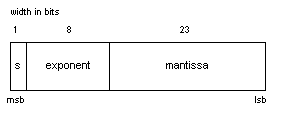
\epsfig{file=pics/single.png}
\else
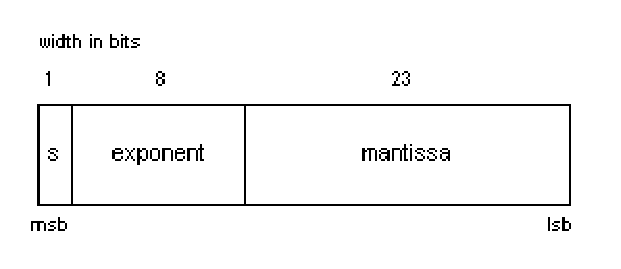
\epsfig{file=pics/single.eps}
\fi
\end{center}
\end{figure}
\end{latexonly}


\subsubsection{double}

The \var{double} type occupies 8 bytes of storage space,
and its memory structure is the same as the IEEE-754 double
type.

The memory format of the \var{double} format looks like
\begin{htmlonly}
this:
\fpcaddimg{./double.png}
\end{htmlonly}
\begin{latexonly}
like what is shown in \seefig{doubleformat}.
\begin{figure}
\begin{center}
\caption{The double format}
\label{fig:doubleformat}
\ifpdf
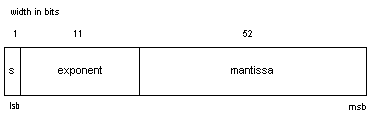
\epsfig{file=pics/double.png}
\else
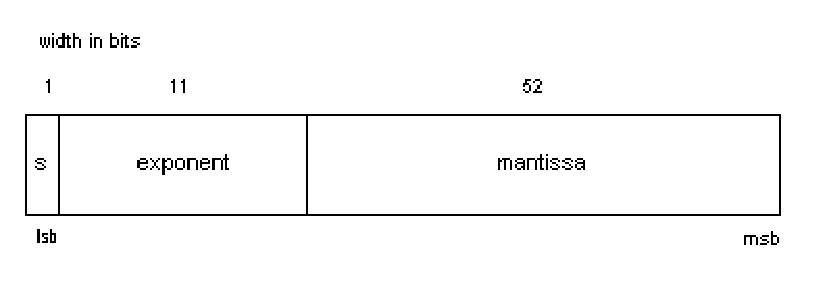
\epsfig{file=pics/double.eps}
\fi
\end{center}
\end{figure}
\end{latexonly}


On processors which do not support co-processor operations (and which have
the \{\$E-\} switch), the \var{double} type does not exist.



\subsubsection{extended}

For Intel 80x86 processors, the \var{extended} type has
takes up 10 bytes of memory space. For more information
on the extended type consult the Intel Programmer's reference.

For all other processors which support floating point operations,
the \var{extended} type is a nickname for the \var{double} type. 
It has the same format and size as the \var{double} type. On
processors which do not support co-processor operations (and which have
the \{\$E-\} switch), the
\var{extended} type does not exist.

\subsubsection{comp}

For Intel 80x86 processors, the \var{comp} type contains
a 63-bit integral value, and a sign bit (in the MSB position).
The \var{comp} type takes up 8 bytes of storage space.

On other processors, the \var{comp} type is not supported.

\subsubsection{real}

Contrary to Turbo Pascal, where the \var{real} type had
a special internal format, under \fpc the \var{real} type
simply maps to one of the other real types. It maps to the
\var{double} type on processors which support floating
point operations, while it maps to the \var{single} type
on processors which do not support floating point operations
in hardware. See \seet{RealMapping} for more information
on this.

\subsection{pointer types}

A \var{pointer} type is stored as a cardinal (unsigned 32-bit value) on
32-bit processors, and is stored as a 64-bit unsigned value\footnote{this
is actually the \var{qword} type, which is not supported in \fpc v1.0}
on 64-bit processors.

\subsection{string types}

\subsubsection{ansistring types}

The ansistring is a dynamically allocated string which
has no length limitation. When the string is no longer
being referenced (its reference count reaches zero),
its memory is automatically freed.

If the ansistring is a constant, then its reference
count will be equal to -1, indicating that it should
never be freed. The structure in memory for an
ansistring is shown in \seet{ansistrings}.

\begin{FPCltable}{rl}{AnsiString memory structure (32-bit model)}{ansistrings}
Offset & Contains \\ \hline
-12  & Longint with maximum string size. \\
-8   & Longint with actual string size.\\
-4   & Longint with reference count.\\
0    & Actual array of \var{char}, null-terminated. \\ \hline
\end{FPCltable}


\subsubsection{shortstring types}

A shortstring occupies as many bytes as its maximum length plus one.
The first byte contains the current dynamic length of the string. The
following bytes contain the actual characters (of type \var{char})
of the string. The maximum size of a short string is the length
byte followed by 255 characters.

\subsubsection{widestring types}

The widestring (composed of unicode characters) is not supported
in \fpc v1.0.

\subsection{set types}

A set is stored as an array of bits, where each bit indicates
if the element is in the set or excluded from the set. The maximum
number of elements in a set is 256.

If a set has less than 32 elements, it is coded as an unsigned
32-bit value. Otherwise it is coded as a 8 element array of
32-bit unsigned values (cardinal) (hence a size of 256 bytes).

The cardinal number of a specific element \var{E} is given by :

\begin{verbatim}
 CardinalNumber = (E div 32);
\end{verbatim}

and the bit number within that 32-bit value is given by:
\begin{verbatim}
 BitNumber = (E mod 32);
\end{verbatim}

\subsection{array types}

An array is stored as a contiguous sequence of variables
of the components of the array. The components with the
lowest indexes are stored first in memory. No alignment
is done between each element of the array. A multi-dimensional
array is stored with the rightmost dimension increasing first.

\subsection{record types}

Each field of a record are stored in a contigous sequence
of variables, where the first field is stored at the
lowest address in memory. In case of variant fields in
a record, each variant starts at the same address in
memory. Fields of record are usually aligned, unless
the \var{packed} directive is specified when declaring
the record type. For more information on field alignment,
consult \sees{StructuredAlignment}.

%%%%%%%%%%%%%%%%%%%%%%%%%%%%%%%%%%%%%%%%%%%%%%%%%%%%%%%%%%%%%%%%%%%%%
% memory storage of Objects
\subsection{object types}
\label{subse:ObjMemory}

Objects are stored in memory just as ordinary records with an extra field:
a pointer to the Virtual Method Table (VMT). This field is stored first, and
all fields in the object are stored in the order they are declared (with possible
alignment of field addresses, unless the object was declared as being \var{packed}).

This field is initialized by the call to the object's \var{Constructor} method.
If the \var{new} operator was used to call the constructor, the data fields
of the object will be stored in heap memory, otherwise they will directly
be stored in the data section of the final executable.

If an object doesn't have virtual methods, no pointer to a VMT is inserted.

The memory allocated looks as in \seet{ObjMem}.
\begin{FPCltable}{ll}{Object memory layout (32-bit model)}{ObjMem} \hline
Offset & What \\ \hline
+0 & Pointer to VMT (optional). \\
+4 & Data. All fields in the order the've been declared. \\
\dots & \\
\hline
\end{FPCltable}

The Virtual Method Table (VMT) for each object type consists of 2 check
fields  (containing the size of the data), a pointer to the object's ancestor's
VMT (\var{Nil} if there is no ancestor), and then the pointers to all virtual
methods. The VMT layout is illustrated in \seet{ObjVMTMem}. The VMT is
constructed by the compiler.

\begin{FPCltable}{ll}{Object Virtual Method Table memory layout (32-bit model)}{ObjVMTMem} \hline
Offset & What \\ \hline
+0 & Size of object type data \\
+4 & Minus the size of object type data. Enables determining of valid VMT
pointers. \\
+8 & Pointer to ancestor VMT, \var{Nil} if no ancestor available.\\
+12 & Pointers to the virtual methods. \\
\dots & \\
\hline
\end{FPCltable}


\subsection{class types}

Just like objects, classes are stored in memory just as ordinary records
with an extra field: a pointer to the Virtual Method Table (VMT).
This field is stored first, and all fields in the class are stored in
the order they are declared.

Contrary to objects, all data fields of a class are always stored
in heap memory.

The memory allocated looks as in \seet{ClassMem}.
\begin{FPCltable}{ll}{Class memory layout (32-bit model)}{ClassMem} \hline
Offset & What \\ \hline
+0 & Pointer to VMT. \\
+4 & Data. All fields in the order the've been declared. \\
\dots & \\
\hline
\end{FPCltable}

The Virtual Method Table (VMT) of each class consists of several fields,
which are used for runtime type information. The VMT layout is illustrated
in \seet{ClassVMTMem}. The VMT is constructed by the compiler.

\begin{FPCltable}{ll}{Class Virtual Method Table memory layout (32-bit model)}{ClassVMTMem} \hline
Offset & What \\ \hline
+0 & Size of object type data \\
+4 & Minus the size of object type data. Enables determining of valid VMT
pointers. \\
+8 & Pointer to ancestor VMT, \var{Nil} if no ancestor available.\\
+12 & Pointer to the class name (stored as a \var{shortstring}). \\
+16 & Pointer to the dynamic method table (using \var{message} with integers).\\
+20 & Pointer to the method definition table. \\
+24 & Pointer to the field definition table. \\
+28 & Pointer to type information table. \\
+32 & Pointer to instance initialization table. \\
+36 & Reserved.\\
+40 & Pointer to the interface table. \\
+44 & Pointer to the dynamic method table (using \var{message} with strings).\\
+48 & Pointer to the \var{Destroy} destructor. \\
+52 & Pointer to the \var{NewInstance} method. \\
+56 & Pointer to the \var{FreeInstance} method. \\
+60 & Pointer to the \var{SafeCallException} method. \\
+64 & Pointer to the \var{DefaultHandler} method. \\
+68 & Pointer to the \var{AfterConstruction} method. \\
+72 & Pointer to the \var{BeforeDestruction} method. \\
+76 & Pointer to the \var{DefaultHandlerStr} method. \\
+80 & Pointers to other virtual methods. \\
\dots & \\
\hline
\end{FPCltable}

\subsection{file types}

File types are represented as records. Typed files and untyped
files are represented as a fixed record:

\begin{verbatim}
  filerec = packed record
    handle    : longint;
    mode      : longint;
    recsize   : longint;
    _private  : array[1..32] of byte;
    userdata  : array[1..16] of byte;
    name      : array[0..255] of char;
  End;
\end{verbatim}

Text files are described using the following record:

\begin{verbatim}
  TextBuf = array[0..255] of char;
  textrec = packed record
    handle    : longint;
    mode      : longint;
    bufsize   : longint;
    _private  : longint;
    bufpos    : longint;
    bufend    : longint;
    bufptr    : ^textbuf;
    openfunc  : pointer;
    inoutfunc : pointer;
    flushfunc : pointer;
    closefunc : pointer;
    userdata  : array[1..16] of byte;
    name      : array[0..255] of char;
    buffer    : textbuf;
  End;
\end{verbatim}

\begin{description}
\item[handle] The handle field returns the file handle (if the file is
opened), as returned by the operating system.

\item[mode] The mode field can take one of several values. When it is
\var{fmclosed}, then the file is closed, and the \var{handle} field is invalid.
When the value is equal to \var{fminput}, it indicates that the file is
opened for read only access. \var{fmoutput} indicates write only access,
and the \var{fminout} indicates read-write access to the file.

\item[name] The \var{name} field is a null terminated character string representing
the name of the file.

\item[userdata] The \var{userdata} field is never used by \fpc, and can
be used for special purposes by software developpers.

\end{description}

\subsection{procedural types}

A procedural type is stored as a generic pointer, which stores
the address of the routine.

%%%%%%%%%%%%%%%%%%%%%%%%%%%%%%%%%%%%%%%%%%%%%%%%%%%%%%%%%%%%%%%%%%%%%
% The alignment of data elements
\section{Data alignment}
\label{se:Alignment}

\subsection{Typed constants and variable alignment}

All static data (variables and typed constants) which are greater than
a byte are usually aligned on a power of two boundary. This alignment
applies only to the start address of the variables, and not the alignment
of fields within structures or objects for example. For more information
on structured alignment, \sees{StructuredAlignment}. The alignment
is similar across the different target processors. \footnote{The Intel
80x86 version does not align data in the case of constant strings,
constant sets, constant floating point values amd global variables.
This will be fixed in the version 1.1 release.}


\begin{FPCltable}{lccc}{Data alignment}{DataAlignment}
\hline
Data size (bytes) & Alignment (small size) & Alignment (fast)\\
1 & 1 & 1\\
2-3 & 2 & 2\\
4-7 & 2 & 4\\
8+ & 2 & 4\\
\hline
\end{FPCltable}


The alignment columns indicates the address alignment of the variable,
i.e the start address of the variable will be aligned on that boundary.
The small size alignment is valid when the code generated should be
optimized for size (\var{-Og} compiler option) and not speed, otherwise and
by default, the fast alignment is used to align the data.

\subsection{Structured types alignment}
\label{se:StructuredAlignment}

By default all elements in a structure are aligned to a 2 byte boundary,
unless the {\var{\$PACKRECORDS} directive or \var{packed} modifier is used
to align the data in another way. For example a \var{record} or \var{object}
having a 1 byte element, will have its size rounded up to 2, so the size of
the structure will actually be 2 bytes.

%%%%%%%%%%%%%%%%%%%%%%%%%%%%%%%%%%%%%%%%%%%%%%%%%%%%%%%%%%%%%%%%%%%%%
% The heap
\section{The heap}
\label{se:Heap}
The heap is used to store all dynamic variables, and to store class
instances. The interface to the heap is the same as in Turbo Pascal,
although the effects are maybe not the same. On top of that, the \fpc
run-time library has some extra possibilities, not available in Turbo
Pascal. These extra possibilities are explained in the next subsections.

% The heap algorithm
\subsection{Heap allocation strategy}


The heap is a memory structure which is organized as a stack. The heap
bottom is stored in the variable \var{HeapOrg}. Initially the heap
pointer (\var{HeapPtr}) points to the bottom of the heap. When a
variable is allocated on the heap, \var{HeapPtr} is incremented by the
size of the allocated memory block. This has the effect of stacking
dynamic variables on top of each other.

Each time a block is allocated, its size is normalized to have
a granularity of 16 bytes.

When \var{Dispose} or \var{FreeMem} is called to dispose of a
memory block which is not on the top of the heap, the heap becomes
fragmented. The deallocation routines also add the freed blocks to
the \var{freelist} which is actually a linked list of free blocks.
Furthermore, if the deallocated block was less then 8K in size, the
free list cache is also updated.

The free list cache is actually a cache of free heap blocks which
have specific lengths (the adjusted block size divided by 16 gives the
index into the free list cache table). It is faster to access then
searching through the entire \var{freelist}.

The format of an entry in the \var{freelist} is as follows:

\begin{verbatim}
 PFreeRecord = ^TFreeRecord;
 TFreeRecord = record
   Size : longint;
   Next : PFreeRecord;
   Prev : PFreeRecord;
 end;

\end{verbatim}

The \var{Next} field points to the next free block, while
the \var{Prev} field points to the previous free block.

The algorithm for allocating memory is as follows:

\begin{enumerate}
\item The size of the block to allocate is adjusted to a 16 byte granularity.
\item The cached free list is searched to find a free block of the specified
 size or bigger size, if so it is allocated and the routine exits.
\item The \var{freelist} is searched to find a free block of the specified size
or of bigger size, if so it is allocated and the routine exits.
\item If not found in the \var{freelist} the heap is grown to allocate the
specified memory, and the routine exits.
\item If the heap cannot be grown internally anymore and if \var{heaperror} is set
accordingly, it calls the heap error handler. If there is no heap error handler
installed, the runtime library generates a runtime error 203.
\end{enumerate}


% Error handler routinr
\subsection{The HeapError variable}

The heap error permits developpers to install a heap error hook which
is called each time an allocation cannot be completed by the default
heap manager. \var{HeapError} is a pointer that points to a function
with the following prototype:

\begin{verbatim}
  function HeapFunc(size : longint): integer;
\end{verbatim}

The \var{size} parameter indicates the size of the block which could
not be allocated. Depending on the success, the error handler routine
should return a value which indicates what the default heap manager
should do thereafter (cf. \seet{Heaperrorresult}).

\begin{FPCltable}{|c|l|}{Heap error result}{Heaperrorresult}
\hline
 Value returned & Memory manager action \\
 \hline
     0		& Generates a runtime error 203 \\
     1		& \var{GetMem} and \var{New} returns \var{nil} \\
     2		& Try allocating the memory block once again \\
\hline
\end{FPCltable}



% The heap grows
\subsection{The heap grows}
By default, \var{HeapError} points to the \var{GrowHeap} function,
which tries to increase the heap.

The \var{GrowHeap} function issues a system call to try to increase the size of the
memory available to your program. It first tries to increase memory in a 256Kb
chunk if the size to allocate is less than 256Kb, or 1024K otherwise.
If this fails, it tries to increase the heap by the amount you requested
from the heap.

If the call to \var{GrowHeap} was successful, then the needed memory will be
allocated.

If the call to \var{GrowHeap} fails, the value returned depends on the
value of the \var{ReturnNilIfGrowHeapFails} global variable. This is summarized
in \seet{growheapnil}.

\begin{FPCltable}{|c|l|}{ReturnNilIfGrowHeapFails value}{growheapnil}
\hline
  ReturnNilGrowHeapFails & Default memory \\
    value		 & manager action \\
\hline  
     FALSE	        & (The default) Runtime error 203 generated \\
     TRUE 		& \var{GetMem} and \var{New} returns \var{nil} \\
\hline
\end{FPCltable}

\var{ReturnNilIfGrowHeapFails} can be set to change the behavior of 
the default memory manager error handler.

%%%%%%%%%%%%%%%%%%%%%%%%%%%%%%%%%%%%%%%%%%%%%%%%%%%%%%%%%%%%%%%%%%%%%%%
% Debugging the heap
\subsection{Debugging the heap}

\fpc provides a unit that allows you to trace allocation and deallocation
of heap memory: \file{heaptrc}.

If you specify the \var{-gh} switch on the command-line, or if you include
\var{heaptrc} as the first unit in your uses clause, the memory manager
will trace what is allocated and deallocated, and on exit of your program,
a summary will be sent to standard output.

More information on using the \var{heaptrc} mechanism can be found in the
\userref and \unitsref.

%%%%%%%%%%%%%%%%%%%%%%%%%%%%%%%%%%%%%%%%%%%%%%%%%%%%%%%%%%%%%%%%%%%%%%%
% Writing your own memory manager.
\subsection{Writing your own memory manager}

\fpc allows you to write and use your own memory manager. The standard
functions \var{GetMem}, \var{FreeMem}, \var{ReallocMem} and \var{Maxavail}
use a special record in the \file{system} unit to do the actual memory management.
The \file{system} unit initializes this record with the \file{system} unit's own memory
manager, but you can read and set this record using the
\var{GetMemoryManager} and \var{SetMemoryManager} calls:
\begin{verbatim}
procedure GetMemoryManager(var MemMgr: TMemoryManager);
procedure SetMemoryManager(const MemMgr: TMemoryManager);
\end{verbatim}

the \var{TMemoryManager} record is defined as follows:
\begin{verbatim}
  TMemoryManager = record
    Getmem      : Function(Size:Longint):Pointer;
    Freemem     : Function(var p:pointer):Longint;
    FreememSize : Function(var p:pointer;Size:Longint):Longint;
    AllocMem    : Function(Size:longint):Pointer;
    ReAllocMem  : Function(var p:pointer;Size:longint):Pointer;
    MemSize     : function(p:pointer):Longint;
    MemAvail    : Function:Longint;
    MaxAvail    : Function:Longint;
    HeapSize    : Function:Longint;
  end;
\end{verbatim}

As you can see, the elements of this record are procedural variables.
The \file{system} unit does nothing but call these various variables when you
allocate or deallocate memory.

Each of these functions corresponds to the corresponding call in the \file{system}
unit. We'll describe each one of them:
\begin{description}
\item[Getmem] This function allocates a new block on the heap. The block
should be \var{Size} bytes long. The return value is a pointer to the newly
allocated block.
\item[Freemem] should release a previously allocated block. The pointer
\var{P} points to a previously allocated block. The Memory manager should
implement a mechanism to determine what the size of the memory block is
\footnote{By storing it's size at a negative offset for instance.} The
return value is optional, and can be used to return the size of the freed
memory.
\item[FreememSize] This function should release the memory pointed to by
\var{P}. The argument \var{Size} is the expected size of the memory block
pointed to by P. This should be disregarded, but can be used to check the
behaviour of the program.
\item[AllocMem] Is the same as getmem, only the allocated memory should
be filled with zeroes before the call returns.
\item[ReAllocMem] Should allocate a memory block \var{Size} bytes large,
and should fill it with the contents of the memory block pointed to by
\var{P}, truncating this to the new size of needed. After that, the memory
pointed to by P may be deallocated. The return value is a pointer to the
new memory block.
\item[MemSize] should return the total amount of memory available for
allocation. This function may return zero if the memory manager does not
allow to determine this information.
\item[MaxAvail] should return the size of the largest block of memory that
is still available for allocation. This function may return zero if the
memory manager does not allow to determine this information.
\item[HeapSize] should return the total size of the heap. This may be zero
is the memory manager does not allow to determine this information.
\end{description}
To implement your own memory manager, it is sufficient to construct such a
record and to issue a call to \var{SetMemoryManager}.

To avoid conflicts with the system memory manager, setting the memory
manager should happen as soon as possible in the initialization of your
program, i.e. before any call to \var{getmem} is processed.

This means in practice that the unit implementing the memory manager should
be the first in the \var{uses} clause of your program or library, since it
will then be initialized before all other units (except of the \file{system} unit)

This also means that it is not possible to use the \file{heaptrc} unit in
combination with a custom memory manager, since the \file{heaptrc} unit uses
the system memory manager to do all it's allocation. Putting the
\file{heaptrc} unit after the unit implementing the memory manager would
overwrite the memory manager record installed by the custom memory manager,
and vice versa.

The following unit shows a straightforward implementation of a custom
memory manager using the memory manager of the \var{C} library. It is
distributed  as a package with \fpc.
\begin{verbatim}
unit cmem;

{$mode objfpc}

interface

Function Malloc (Size : Longint) : Pointer;cdecl;
  external 'c' name 'malloc';
Procedure Free (P : pointer); cdecl; external 'c' name 'free';
Procedure FreeMem (P : Pointer); cdecl; external 'c' name 'free';
function ReAlloc (P : Pointer; Size : longint) : pointer; cdecl;
  external 'c' name 'realloc';
Function CAlloc (unitSize,UnitCount : Longint) : pointer;cdecl;
  external 'c' name 'calloc';

implementation

Function CGetMem  (Size : Longint) : Pointer;

begin
  result:=Malloc(Size);
end;

Function CFreeMem (Var P : pointer) : Longint;

begin
  Free(P);
  Result:=0;
end;

Function CFreeMemSize(var p:pointer;Size:Longint):Longint;

begin
  Result:=CFreeMem(P);
end;

Function CAllocMem(Size : Longint) : Pointer;

begin
  Result:=calloc(Size,1);
end;

Function CReAllocMem (var p:pointer;Size:longint):Pointer;

begin
  Result:=realloc(p,size);
end;

Function CMemSize (p:pointer): Longint;

begin
  Result:=0;
end;

Function CMemAvail : Longint;

begin
  Result:=0;
end;

Function CMaxAvail: Longint;

begin
  Result:=0;
end;

Function CHeapSize : Longint;

begin
  Result:=0;
end;


Const
 CMemoryManager : TMemoryManager =
    (
      GetMem : CGetmem;
      FreeMem : CFreeMem;
      FreememSize : CFreememSize;
      AllocMem : CAllocMem;
      ReallocMem : CReAllocMem;
      MemSize : CMemSize;
      MemAvail : CMemAvail;
      MaxAvail : MaxAvail;
      HeapSize : CHeapSize;
    );

Var
  OldMemoryManager : TMemoryManager;

Initialization
  GetMemoryManager (OldMemoryManager);
  SetMemoryManager (CmemoryManager);

Finalization
  SetMemoryManager (OldMemoryManager);
end.
\end{verbatim}

%%%%%%%%%%%%%%%%%%%%%%%%%%%%%%%%%%%%%%%%%%%%%%%%%%%%%%%%%%%%%%%%%%%%%
% Accessing DOS memory under the GO32 extender
\section{Using \dos memory under the Go32 extender}
\label{se:AccessingDosMemory}

Because \fpc for \dos is a 32 bit compiler, and uses a \dos extender, accessing DOS
memory isn't trivial. What follows is an attempt to an explanation of how to
access and use \dos or real mode memory\footnote{Thanks for the explanation to
Thomas Schatzl (E-mail: \var{tom\_at\_work@geocities.com})}.

In {\em Proteced Mode}, memory is accessed through {\em Selectors} and
{\em Offsets}. You can think of Selectors as the protected mode
equivalents of segments.

In \fpc, a pointer is an offset into the \var{DS} selector, which points to
the Data of your program.

To access the (real mode) \dos memory, somehow you need a selector that
points to the \dos memory.
The \file{go32} unit provides you with such a selector: The
\var{DosMemSelector} variable, as it is conveniently called.

You can also allocate memory in \dos's memory space, using the
\var{global\_dos\_alloc} function of the \file{go32} unit.
This function will allocate memory in a place where \dos sees it.

As an example, here is a function that returns memory in real mode \dos and
returns a selector:offset pair for it.
\begin{verbatim}
procedure dosalloc(var selector : word;
                   var segment : word;
                   size : longint);

var result : longint;

begin
     result := global_dos_alloc(size);
     selector := word(result);
     segment := word(result shr 16);
end;
\end{verbatim}
(You need to free this memory using the \var{global\_dos\_free} function.)

You can access any place in memory using a selector. You can get a selector
using the \var{allocate\_ldt\_descriptor} function, and then let this selector
point to the physical memory you want using the
\var{set\_segment\_base\_address} function, and set its length using
\var{set\_segment\_limit} function.
You can manipulate the memory pointed to by the selector using the functions
of the GO32 unit. For instance with the \var{seg\_fillchar} function.
After using the selector, you must free it again using the
\var{free\_ldt\_selector} function.

More information on all this can be found in the \unitsref, the chapter on
the \file{go32} unit.



%%%%%%%%%%%%%%%%%%%%%%%%%%%%%%%%%%%%%%%%%%%%%%%%%%%%%%%%%%%%%%%%%%%%%%%
% Resource strings
%%%%%%%%%%%%%%%%%%%%%%%%%%%%%%%%%%%%%%%%%%%%%%%%%%%%%%%%%%%%%%%%%%%%%%%
\chapter{Resource strings}
\label{resourcestrings}
\section{Introduction}
Resource strings primarily exist to make internationalization of
applications easier, by introducing a language construct that provides
a uniform way of handling constant strings.

Most applications communicate with the user through some messages on the
graphical screen or console. Storing these messages in special constants
allows to store them in a uniform way in separate files, which can be used
for translation. A programmers interface exists to manipulate the actual
values of the constant strings at runtime, and a utility tool comes with the
Free Pascal compiler to convert the resource string files to whatever format
is wanted by the programmer. Both these things are discussed in the
following sections.

\section{The resource string file}
When a unit is compiled that contains a \var{resourcestring} section,
the compiler does 2 things:
\begin{enumerate}
\item It generates a table that contains the value of the strings as it
is declared in the sources.
\item It generates a {\em resource string file} that contains the names
of all strings, together with their declared values.
\end{enumerate}
This approach has 2 advantages: first of all, the value of the string is
always present in the program. If the programmer doesn't care to translate
the strings, the default values are always present in the binary. This also
avoids having to provide a file containing the strings. Secondly, having all
strings together in a compiler generated file ensures that all strings are
together (you can have multiple resourcestring sections in 1 unit or program)
and having this file in a fixed format, allows the programmer to choose his
way of internationalization.

For each unit that is compiled and that contains a resourcestring section,
the compiler generates a file that has the name of the unit, and an
extension \file{.rst}. The format of this file is as follows:
\begin{enumerate}
\item An empty line.
\item A line starting with a hash sign (\var{\#}) and the hash value of the
  string, preceded by the text \var{hash value =}.
\item A third line, containing the name of the resource string in the format
\var{unitname.constantname}, all lowercase, followed by an equal sign, and
the string value, in a format equal to the pascal representation of this
string. The line may be continued on the next line, in that case it reads as
a pascal string expression with a plus sign in it.
\item Another empty line.
\end{enumerate}
If the unit contains no \var{resourcestring} section, no file is generated.

For example, the following unit:
\begin{verbatim}
unit rsdemo;

{$mode delphi}
{$H+}

interface

resourcestring

  First = 'First';
  Second = 'A Second very long string that should cover more than 1 line';


implementation

end.
\end{verbatim}
Will result in the following resource string file:
\begin{verbatim}

# hash value = 5048740
rsdemo.first='First'


# hash value = 171989989
rsdemo.second='A Second very long string that should cover more than 1 li'+
'ne'

\end{verbatim}
The hash value is calculated with the function \var{Hash}. It is present in
the \file{objpas} unit. The value is the same value that the GNU gettext
mechanism uses. It is in no way unique, and can only be used to speed up
searches.

The \file{rstconv} utility that comes with the \fpc compiler allows to
manipulate these resource string files. At the moment, it can only be used
to make a \file{.po} file that can be fed to the GNU \file{msgfmt} program.
If someone wishes to have another format (Win32 resource files spring to
mind), one can enhance the \file{rstconv} program so it can generate
other types of files as well. GNU gettext was chosen because it is available
on all platforms, and is already widely used in the \var{Unix} and free
software community. Since the \fpc team doesn't want to restrict the use
of resource strings, the \file{.rst} format was chosen to provide a neutral
method, not restricted to any tool.

If you use resource strings in your units, and you want people to be able to
translate the strings, you must provide the resource string file. Currently,
there is no way to extract them from the unit file, though this is in
principle possible. It is not required to do this, the program can be
compiled without it, but then the translation of the strings isn't possible.

\section{Updating the string tables}
Having compiled a program with resourcestrings is not enough to
internationalize your program. At run-time, the program must initialize
the string tables with the correct values for the anguage that the user
selected. By default no such initialization is performed. All strings
are initialized with their declared values.

The \file{objpas} unit provides the mechanism to correctly initialize
the string tables. There is no need to include this unit in a \var{uses}
clause, since it is automatically loaded when a program or unit is
compiled in \var{Delphi} or \var{objfpc} mode. Since this is required
to use resource strings, the unit is always loaded when needed.

The resource strings are stored in tables, one per unit, and one for the
program, if it contains a \var{resourcestring} section as well. Each
resourcestring is stored with it's name, hash value, default value, and
the current value, all as \var{AnsiStrings}.

The objpas unit offers methods to retrieve the number of resourcestring
tables, the number of strings per table, and the above information for each
string. It also offers a method to set the current value of the strings.

Here are the declarations of all the functions:
\begin{verbatim}
Function ResourceStringTableCount : Longint;
Function ResourceStringCount(TableIndex : longint) : longint;
Function GetResourceStringName(TableIndex,
                               StringIndex : Longint) : Ansistring;
Function GetResourceStringHash(TableIndex,
                               StringIndex : Longint) : Longint;
Function GetResourceStringDefaultValue(TableIndex,
                                       StringIndex : Longint) : AnsiString;
Function GetResourceStringCurrentValue(TableIndex,
                                       StringIndex : Longint) : AnsiString;
Function SetResourceStringValue(TableIndex,
                                StringIndex : longint;
                                Value : Ansistring) : Boolean;
Procedure SetResourceStrings (SetFunction :  TResourceIterator);
\end{verbatim}
Two other function exist, for convenience only:
\begin{verbatim}
Function Hash(S : AnsiString) : longint;
Procedure ResetResourceTables;
\end{verbatim}
Here is a short explanation of what each function does. A more detailed
explanation of the functions can be found in the \refref.
\begin{description}
\item[ResourceStringTableCount] returns the number of resource string tables
in the program.
\item[ResourceStringCount] returns the number of resource string entries in
a given table (tables are denoted by a zero-based index).
\item[GetResourceStringName] returns the name of a resource string in a
resource table. This is the name of the unit, a dot (.) and the name of
the string constant, all in lowercase. The strings are denoted by index,
also zero-based.
\item[GetResourceStringHash] returns the hash value of a resource string, as
calculated by the compiler with the \var{Hash} function.
\item[GetResourceStringDefaultValue] returns the default value of a resource
string, i.e. the value that appears in the resource string declaration, and
that is stored in the binary.
\item[GetResourceStringCurrentValue] returns the current value of a resource
string, i.e. the value set by the initialization (the default value), or the
value set by some previous internationalization routine.
\item[SetResourceStringValue] sets the current value of a resource string.
This function must be called to initialize all strings.
\item[SetResourceStrings] giving this function a callback will cause the
calback to be called for all resource strings, one by one, and set the value
of the string to the return value of the callback.
\end{description}
Two other functions exist, for convenience only:
\begin{description}
\item [Hash] can be used to calculate the hash value of a string. The hash
value stored in the tables is the result of this function, applied on the
default value. That value is calculated at compile time by the compiler.
\item[ResetResourceTables] will reset all the resource strings to their
default values. It is called by the initialization code of the objpas unit.
\end{description}

Given some \var{Translate} function, the following code would initialize
all resource strings:
\begin{verbatim}
Var I,J : Longint;
    S : AnsiString;

begin
  For I:=0 to ResourceStringTableCount-1 do
    For J:=0 to ResourceStringCount(i)-1 do
      begin
      S:=Translate(GetResourceStringDefaultValue(I,J));
      SetResourceStringValue(I,J,S);
      end;
end;
\end{verbatim}
Other methods are of course possible, and the \var{Translate} function
can be implemented in a variety of ways.
\section{GNU gettext}
The unit \file{gettext} provides a way to internationalize an application
with the GNU \file{gettext} utilities. This unit is supplied with  the
Free Component Library (FCL). it can be used as follows:

for a given application, the following steps must be followed:
\begin{enumerate}
\item Collect all resource string files and concatenate them together.
\item Invoke the \file{rstconv} program with the file resulting out of step
1, resulting in a single \file{.po} file containing all resource strings of
the program.
\item Translate the \file{.po} file of step 2 in all required languages.
\item Run the \file{msgfmt} formatting program on all the \file{.po} files,
resulting in a set of \file{.mo} files, which can be distributed with your
application.
\item Call the \file{gettext} unit's \var{TranslateReosurceStrings} method,
giving it a template for the location of the \file{.mo} files, e.g. as in
\begin{verbatim}
TranslateResourcestrings('intl/restest.%s.mo');
\end{verbatim}
the \var{\%s} specifier will be replaced by the contents of the \var{LANG}
environment variable. This call should happen at program startup.
\end{enumerate}
An example program exists in the FCL sources, in the \file{fcl/tests}
directory.
\section{Caveat}
In principle it is possible to translate all resource strings at any time in
a running program. However, this change is not communicated to other
strings; its change is noticed only when a constant string is being used.

Consider the following example:
\begin{verbatim}
Const
  help = 'With a little help of a programmer.';

Var
  A : AnsiString;


begin

  { lots of code }

  A:=Help;

  { Again some code}

  TranslateStrings;

  { More code }
\end{verbatim}
After the call to \var{TranslateStrings}, the value of \var{A} will remain
unchanged. This means that the assignment \var{A:=Help} must be executed
again in order for the change to become visible. This is important,
especially for GUI programs which have e.g. a menu. In order for the
change in resource strings to become visible, the new values must be
reloaded by program code into the menus \dots

%%%%%%%%%%%%%%%%%%%%%%%%%%%%%%%%%%%%%%%%%%%%%%%%%%%%%%%%%%%%%%%%%%%%%
% Optimizations done in the compiler
%%%%%%%%%%%%%%%%%%%%%%%%%%%%%%%%%%%%%%%%%%%%%%%%%%%%%%%%%%%%%%%%%%%%%
\chapter{Optimizations}

\section{Non processor specific}

The following sections describe the general optimizations
done by the compiler, they are not processor specific. Some
of these require some compiler switch override while others are done
automatically (those which require a switch will be noted as such).

\subsection{Constant folding}

In \fpc, if the operand(s) of an operator are constants, they
will be evaluated at compile time.

Example

\begin{verbatim}
   x:=1+2+3+6+5;
\end{verbatim}
will generate the same code as
\begin{verbatim}
   x:=17;
\end{verbatim}

Furthermore, if an array index is a constant, the offset will
be evaluated at compile time. This means that accessing MyData[5]
is as efficient as accessing a normal variable.

Finally, calling \var{Chr}, \var{Hi}, \var{Lo}, \var{Ord}, \var{Pred},
or \var{Succ} functions with constant parameters generates no
run-time library calls, instead, the values are evaluated at
compile time.

\subsection{Constant merging}

Using the same constant string, floating point value or constant set 
two or more times generates only one copy of that constant.

\subsection{Short cut evaluation}

Evaluation of boolean expression stops as soon as the result is
known, which makes code execute faster then if all boolean operands
were evaluated.

\subsection{Constant set inlining}

Using the \var{in} operator is always more efficient then using the
equivalent \verb|<>|, \verb|=|, \verb|<=|, \verb|>=|, \verb|<| and \verb|>|
operators. This is because range comparisons can be done more easily with
\var{in} then with normal comparison operators.

\subsection{Small sets}

Sets which contain less then 33 elements can be directly encoded
using a 32-bit value, therefore no run-time library calls to
evaluate operands on these sets are required; they are directly encoded
by the code generator.

\subsection{Range checking}

Assignments of constants to variables are range checked at compile
time, which removes the need of the generation of runtime range checking
code.

\subsection{And instead of modulo}

When the second operand of a \var{mod} on an unsigned value is a constant
power of 2, an \var{and} instruction is used instead of an integer division.
This generates more efficient code.

\subsection{Shifts instead of multiply or divide}

When one of the operands in a multiplication is a power of
two, they are encoded using arithmetic shift instructions,
which generates more efficient code.

Similarly, if the divisor in a \var{div} operation is a power
of two, it is encoded using arithmetic shift instructions.

The same is true when accessing array indexes which are
powers of two, the address is calculated using arithmetic
shifts instead of the multiply instruction.

\subsection{Automatic alignment}

By default all variables larger then a byte are guaranteed to be aligned
at least on a word boundary.

Alignment on the stack and in the data section is processor dependant.

\subsection{Smart linking}

This feature removes all unreferenced code in the final executable
file, making the executable file much smaller.

Smart linking is switched on with the \var{-Cx} command-line switch, or
using the \var{\{\$SMARTLINK ON\}} global directive.

\subsection{Inline routines}

The following runtime library routines are coded directly into the
final executable: \var{Lo}, \var{Hi}, \var{High}, \var{Sizeof},
\var{TypeOf}, \var{Length}, \var{Pred}, \var{Succ}, \var{Inc},
\var{Dec} and \var{Assigned}.

\subsection{Stack frame omission}

Under specific conditions, the stack frame (entry and exit code for
the routine, see section \sees{CallingConventions}) will be omitted, and the
variable will directly be accessed via the stack pointer.

Conditions for omission of the stack frame:

\begin{itemize}
\item The function has no parameters nor local variables.
\item Routine is declared with the \var{assembler} modifier.
\item Routine is not a class.
\end{itemize}

\subsection{Register variables}

When using the \var{-Or} switch, local variables or parameters
which are used very often will be moved to registers for faster
access.

\section{Processor specific}

This lists the low-level optimizations performed, on a processor
per processor basis.

\subsection{Intel 80x86 specific}

Here follows a listing of the optimizing techniques used in the compiler:
\begin{enumerate}
\item When optimizing for a specific Processor (\var{-Op1, -Op2, -Op3},
the following is done:
\begin{itemize}
\item In \var{case} statements, a check is done whether a jump table
or a sequence of conditional jumps should be used for optimal performance.
\item Determines a number of strategies when doing peephole optimization, e.g.:
\var{movzbl (\%ebp), \%eax} will be changed into
\var{xorl \%eax,\%eax; movb (\%ebp),\%al } for Pentium and PentiumMMX.
\end{itemize}
\item When optimizing for speed (\var{-OG}, the default) or size (\var{-Og}), a choice is
made between using shorter instructions (for size) such as \var{enter \$4},
or longer instructions \var{subl \$4,\%esp} for speed. When smaller size is
requested, data is aligned to minimal boundaries.  When speed is
requested, data is aligned on most efficient boundaries as much as possible.
\item Fast optimizations (\var{-O1}): activate the peephole optimizer
\item Slower optimizations (\var{-O2}): also activate the common subexpression
elimination (formerly called the "reloading optimizer")
\item Uncertain optimizations (\var{-Ou}): With this switch, the common subexpression
elimination algorithm can be forced into making uncertain optimizations.

Although you can enable uncertain optimizations in most cases, for people who
do not understand the following technical explanation, it might be the safest to
leave them off.

% Jonas's own words..
\begin{remark}If uncertain optimizations are enabled, the CSE algortihm assumes
that
\begin{itemize}
\item If something is written to a local/global register or a
procedure/function parameter, this value doesn't overwrite the value to
which a pointer points.
\item If something is written to memory pointed to by a pointer variable,
this value doesn't overwrite the value of a local/global variable or a
procedure/function parameter.
\end{itemize}
% end of quote
\end{remark}
The practical upshot of this is that you cannot use the uncertain
optimizations if you both write and read local or global variables directly and
through pointers (this includes \var{Var} parameters, as those are pointers too).

The following example will produce bad code when you switch on
uncertain optimizations:
\begin{verbatim}
Var temp: Longint;

Procedure Foo(Var Bar: Longint);
Begin
  If (Bar = temp)
    Then
      Begin
        Inc(Bar);
        If (Bar <> temp) then Writeln('bug!')
      End
End;

Begin
  Foo(Temp);
End.
\end{verbatim}
The reason it produces bad code is because you access the global variable
\var{Temp} both through its name \var{Temp} and through a pointer, in this
case using the \var{Bar} variable parameter, which is nothing but a pointer
to \var{Temp} in the above code.

On the other hand, you can use the uncertain optimizations if
you access global/local variables or parameters through pointers,
and {\em only} access them through this pointer\footnote{
You can use multiple pointers to point to the same variable as well, that
doesn't matter.}.

For example:
\begin{verbatim}
Type TMyRec = Record
                a, b: Longint;
              End;
     PMyRec = ^TMyRec;


     TMyRecArray = Array [1..100000] of TMyRec;
     PMyRecArray = ^TMyRecArray;

Var MyRecArrayPtr: PMyRecArray;
    MyRecPtr: PMyRec;
    Counter: Longint;

Begin
  New(MyRecArrayPtr);
  For Counter := 1 to 100000 Do
    Begin
       MyRecPtr := @MyRecArrayPtr^[Counter];
       MyRecPtr^.a := Counter;
       MyRecPtr^.b := Counter div 2;
    End;
End.
\end{verbatim}
Will produce correct code, because the global variable \var{MyRecArrayPtr}
is not accessed directly, but only through a pointer (\var{MyRecPtr} in this
case).

In conclusion, one could say that you can use uncertain optimizations {\em
only} when you know what you're doing.
\end{enumerate}

\subsection{Motorola 680x0 specific}

Using the \var{-O2} switch does several optimizations in the
code produced, the most notable being:

\begin{itemize}
\item Sign extension from byte to long will use \var{EXTB}
\item Returning of functions will use \var{RTD}
\item Range checking will generate no run-time calls
\item Multiplication will use the long \var{MULS} instruction, no
runtime library call will be generated
\item Division will use the long \var{DIVS} instruction, no
runtime library call will be generated
\end{itemize}

\section{Optimization switches}
This is where the various optimizing switches and their actions are
described, grouped per switch.

\begin{description}
\item [-On:\ ] with n = 1..3: these switches activate the optimizer.
A higher level automatically includes all lower levels.
\begin{itemize}
\item Level 1 (\var{-O1}) activates the peephole optimizer
 (common instruction sequences are replaced by faster equivalents).
\item Level 2 (\var{-O2}) enables the assembler data flow analyzer,
which allows the common subexpression elimination procedure to
remove unnecessary reloads of registers with values they already contain.
\item Level 3 (\var{-O3}) enables uncertain optimizations. For more info, see -Ou.
\end{itemize}
\item[-OG:\ ]
This causes the code generator (and optimizer, IF activated), to favor
faster, but code-wise larger, instruction sequences (such as
"\verb|subl $4,%esp|") instead of slower, smaller instructions
("\verb|enter $4|").  This is the default setting.

\item[-Og:\ ] This one is exactly the reverse of -OG, and as such these
switches are mutually exclusive: enabling one will disable the other.

\item[-Or:\ ] This setting causes the code generator to
check which variables are used most, so it can keep those in a register.

\item[-Opn:\ ] with n = 1..3: Setting the target processor does NOT
activate the optimizer. It merely influences the code generator and,
if activated, the optimizer:
\begin{itemize}
\item During the code generation process, this setting is used to
decide whether a jump table or a sequence of successive jumps provides
the best performance in a case statement.
\item The peephole optimizer takes a number of decisions based on this
setting, for example it translates certain complex instructions, such
as
\begin{verbatim}
movzbl (mem), %eax|
\end{verbatim}
to a combination of simpler instructions
\begin{verbatim}
xorl %eax, %eax
movb (mem), %al
\end{verbatim}
for the Pentium.
\end{itemize}
\item[-Ou:\ ] This enables uncertain optimizations. You cannot use these
always, however. The previous section explains when they can be used, and
when they cannot be used.
\end{description}

\section{Tips to get faster code}
Here, some general tips for getting better code are presented. They
mainly concern coding style.

\begin{itemize}
\item Find a better algorithm. No matter how much you and the compiler
tweak the code, a quicksort will (almost) always outperform a bubble
sort, for example.

\item Use variables of the native size of the processor you're writing
for. This is currently 32-bit or 64-bit for \fpc, so you are best to
use longint and cardinal variables.

\item Turn on the optimizer.

\item Write your if/then/else statements so that the code in the "then"-part
gets executed most of the time (improves the rate of successful jump prediction).

\item Profile your code (see the -pg switch) to find out where the
bottlenecks are. If you want, you can rewrite those parts in assembler.
You can take the code generated by the compiler as a starting point. When
given the \var{-a} command-line switch, the compiler will not erase the
assembler file at the end of the assembly process, so you can study the
assembler file.

\end{itemize}

\section{Tips to get smaller code}
Here are some tips given to get the smallest code possible.

\begin{itemize}

\item Find a better algorithm.

\item Use the \var{-Og} compiler switch.

\item Regroup global static variables in the same module which have the same
 size together to minimize the number of alignment directives (which increases
 the \var{.bss} and \var{.data} sections unecessarily). Internally this is
 due to the fact that all static data is written to in the assembler file,
 in the order they are declared in the pascal source code.

\item Do not use the \var{cdecl} modifier, as this generates
about 1 additional instruction after each subroutine call.

\item Use the smartlinking options for all your units
(including the \var{system} unit).

\item Do not use ansistrings and exception support, as these require
a lot of code overhead.

\item Turn off range checking and stack-checking.

\end{itemize}




%%%%%%%%%%%%%%%%%%%%%%%%%%%%%%%%%%%%%%%%%%%%%%%%%%%%%%%%%%%%%%%%%%%%%
% programming shared libraries
%%%%%%%%%%%%%%%%%%%%%%%%%%%%%%%%%%%%%%%%%%%%%%%%%%%%%%%%%%%%%%%%%%%%%
\chapter{Programming shared libraries}
\label{ch:libraries}
\section{Introduction}
\fpc supports the creation of shared libraries on several operating
systems. The following table (\seet{DLLSupport}) indicates which
operating systems support the creation of shared libraries.

\begin{FPCltable}{lll}{Shared library support}{DLLSupport} \hline
Operating systems & Library extension & Library prefix \\ \hline
linux   & .so & lib \\
windows & .dll & <none> \\
BeOS    & .so  & lib \\
FreeBSD & .so & lib \\
NetBSD  & .so & lib \\
\hline
\end{FPCltable}

The library prefix column indicates how the names of the libraries are
resolved and created. For example, under \linux, the library name will
alwaus have the \var{lib} prefix when it is created. So if you create a
library called \file{mylib}, under \linux, this will result in the
\file{libmylib.so}. Furthermore, when importing routines from shared
libraries, it is not necessary to give the library prefix or the
filename extension.

In the following sections we discuss how to create a library, and how
to use these libraries in programs.

\section{Creating a library}

Creation of libraries is supported in any mode of the \fpc compiler,
but it may be that the arguments or return values differ if the library is
compiled in 2 different modes.  E.g. if your function expects an
\var{Integer} argument, then the library will expect different integer
sizes if you compile it in Delphi mode or in TP mode.

A library can be created just as a program, only it uses the \var{library}
keyword, and it has an \var{exports} section. The following listing
demonstrates a simple library:

\FPCexample{subs}

The function \var{SubStr} does not have to be declared in the library file
itself. It can also be declared in the interface section of a unit that
is used by the library.

Compilation of this source will result in the creation of a library called
\file{libsubs.so} on \unix systems, or \file{subs.dll} on \windows or \ostwo.
The compiler will take care of any additional linking that is required to create a
shared library.

The library exports one function: \var{SubStr}. The case is important. The
case as it appears in the \var{exports} clause is used to export the
function.

If you want your library to be called from programs compiled with
other compilers, it is important to specify the correct calling
convention for the exported functions. Since the generated programs
by other compilers do not know about the \fpc calling conventions,
your functions would be called incorrectly, resulting in a corrupted
stack.


On \windows, most libraries use the \var{stdcall} convention, so it may be
better to use that one if your library is to be used on \windows systems. On
most \unix systems, the C calling convention is used, therefore the
\var{cdecl} modifier should be used in that case.

\section{Using a library in a pascal program}

In order to use a function that resides in a library, it is sufficient to
declare the function as it exists in the library as an \var{external}
function, with correct arguments and return type. The calling convention
used by the function should be declared correctly as well. The compiler
will then link the library as specified in the \var{external} statement
to your program\footnote{If you omit the library name in the \var{external}
modifier, then you can still tell the compiler to link to that library using
the \var{\{\$Linklib\}} directive.}.

For example, to use the library as defined above from a pascal program, you can use
the following pascal program:
\FPCexample{psubs}
As is shown in the example, you must declare the function as \var{external}.
Here also, it is necessary to specify the correct calling convention (it
should always match the convention as used by the function in the library),
and to use the correct casing for your declaration. Also notice, that
the library importing did not specify the filename extension, nor
was the \var{lib} prefix added.

This program can be compiled without any additional command-switches,
and should run just like that, provided the library is placed where
the system can find it. For example, on \linux, this is \file{/usr/lib} or any
directory listed in the \file{/etc/ld.so.conf} file. On \windows, this
can be the program directory, the \windows system directory, or any directoy
mentioned in the \var{PATH}.

Using the library in this way links the library to your program at compile
time. This means that
\begin{enumerate}
\item The library must be present on the system where the program is
compiled.
\item The library must be present on the system where the program is
executed.
\item Both libraries must be exactly the same.
\end{enumerate}
Or it may simply be that you don't know the name of the function to
be called, you just know the arguments it expects.

It is therefore also possible to load the library at run-time, store
the function address in a procedural variable, and use this procedural
variable to access the function in the library.

The following example demonstrates this technique:
\FPCexample{plsubs}
As in the case of compile-time linking, the crucial thing in this
listing is the declaration of the \var{TSubStrFunc} type.
It should match the declaration of the function you're trying to use.
Failure to specify a correct definition will result in a faulty stack or,
worse still, may cause your program to crash with an access violation.

\section{Using a pascal library from a C program}

\begin{remark}The examples in this section assume a \linux system; similar commands
as the ones below exist for other operating systems, though.
\end{remark}

You can also call a \fpc generated library from a C program:
\Cexample{ctest}
To compile this example, the following command can be used:
\begin{verbatim}
gcc -o ctest ctest.c -lsubs
\end{verbatim}
provided the code is in \file{ctest.c}.

The library can also be loaded dynamically from C, as shown in the following
example:
\Cexample{ctest2}
This can be compiled using the following command:
\begin{verbatim}
gcc -o ctest2 ctest2.c -ldl
\end{verbatim}
\lstset{language=delphi}
The \var{-ldl} tells gcc that the program needs the \file{libdl.so} library
to load dynamical libraries.

%%%%%%%%%%%%%%%%%%%%%%%%%%%%%%%%%%%%%%%%%%%%%%%%%%%%%%%%%%%%%%%%%%%%%
% using resources
%%%%%%%%%%%%%%%%%%%%%%%%%%%%%%%%%%%%%%%%%%%%%%%%%%%%%%%%%%%%%%%%%%%%%

\chapter{Using Windows resources}
\label{ch:windres}

\section{The resource directive \var{\$R}}

Under \windows, you can include resources in your executable or library
using the \var{\{\$R filename\}} directive. These resources can then
be accessed through the standard \windows API calls.

When the compiler encounters a resource directive, it just creates an
entry in the unit \file{.ppu} file; it doesn't link the resource. Only
when it creates a library or executable, it looks for all the resource
files for which it encountered a directive, and tries to link them in.

The default extension for resource files is \file{.res}. When the
filename has as the first character an asterix (\var{*}), the
compiler will replace the asterix with the name of the current unit,
library or program.

\begin{remark}This means that the asterix may only be used after a \var{unit},
\var{library} or \var{program} clause.
\end{remark}

\section{Creating resources}

The \fpc compiler itself doesn't create any resource files; it just
compiles them into the executable. To create resource files, you
can use some GUI tools as the Borland resource workshop; but it is
also possible to use a \windows resource compiler like \gnu
\file{windres}. \file{windres} comes with the \gnu binutils, but the
\fpc distribution also contains a version which you can use.

The usage of windres is straightforward; it reads an input file
describing the resources to create and outputs a resource file.

A typical invocation of \file{windres} would be
\begin{verbatim}
windres -i mystrings.rc -o mystrings.res
\end{verbatim}
this will read the \file{mystrings.rc} file and output a
\file{mystrings.res} resource file.

A complete overview of the windres tools is outside the scope of this
document, but here are some things you can use it for:
\begin{description}
\item[stringtables] that contain lists of strings.
\item[bitmaps] which are read from an external file.
\item[icons] which are also read from an external file.
\item[Version information] which can be viewed with the \windows
explorer.
\item[Menus] Can be designed as resources and used in your GUI
applications.
\item[Arbitrary data] Can be included as resources and read with the
windows API calls.
\end{description}

Some of these will be described below.
\section{Using string tables.}
String tables can be used to store and retrieve large collections of
strings in your application.

A string table looks as follows:
\begin{verbatim}
STRINGTABLE { 1, "hello World !"
              2, "hello world again !"
              3, "last hello world !" }
\end{verbatim}
You can compile this (we assume the file is called \file{tests.rc}) as
follows:
\begin{verbatim}
windres -i tests.rc -o tests.res
\end{verbatim}
And this is the way to retrieve the strings from your program:
\begin{verbatim}
program tests;

{$mode objfpc}

Uses Windows;

{$R *.res}

  Function LoadResourceString (Index : longint): Shortstring;

  begin
    SetLength(Result,LoadString(FindResource(0,Nil,RT_STRING),Index,@Result[1],SizeOf(Result)))
  end;

Var
    I: longint;

begin
  For i:=1 to 3 do
    Writeln (Loadresourcestring(I));
end.
\end{verbatim}
The call to \var{FindResource} searches for the stringtable in the
compiled-in resources. The \var{LoadString} function then reads the
string with index \var{i} out of the table, and puts it in a buffer,
which can then be used. Both calls are in the \file{windows} unit.

\section{Inserting version information}

The win32 API allows to store version information in your binaries.
This information can be made visible with the \windows Explorer, by
right-clicking on the executable or library, and selecting the
'Properties' menu. In the tab 'Version' the version information will
be displayed.

Here is how to insert version information in your binary:
\begin{verbatim}
1 VERSIONINFO
FILEVERSION 4, 0, 3, 17
PRODUCTVERSION 3, 0, 0, 0
FILEFLAGSMASK 0
FILEOS 0x40000
FILETYPE 1
{
 BLOCK "StringFileInfo"
 {
  BLOCK "040904E4"
  {
   VALUE "CompanyName", "Free Pascal"
   VALUE "FileDescription", "Free Pascal version information extractor"
   VALUE "FileVersion", "1.0"
   VALUE "InternalName", "Showver"
   VALUE "LegalCopyright", "GNU Public License"
   VALUE "OriginalFilename", "showver.pp"
   VALUE "ProductName", "Free Pascal"
   VALUE "ProductVersion", "1.0"
  }
 }
}
\end{verbatim}
As you can see, you can insert various kinds of information in the version info
block. The keyword \var{VERSIONINFO} marks the beginning of the version
information resource block. The keywords \var{FILEVERSION},
\var{PRODUCTVERSION} give the actual file version, while the block
\var{StringFileInfo} gives other information that is displayed in the
explorer.

The Free Component Library comes with a unit (\file{fileinfo}) that allows
to extract and view version information in a straightforward and easy manner;
the demo program that comes with it (\file{showver}) shows version information
for an arbitrary executable or DLL.

\section{Inserting an application icon}

When \windows shows an executable in the Explorer, it looks for an icon
in the executable to show in front of the filename, the application
icon.

Inserting an application icon is very easy and can be done as follows
\begin{verbatim}
AppIcon ICON "filename.ico"
\end{verbatim}
This will read the file \file{filename.ico} and insert it in the
resource file.

\section{Using a pascal preprocessor}

Sometimes you want to use symbolic names in your resource file, and
use the same names in your program to access the resources. To accomplish
this, there exists a preprocessor for \file{windres} that understands pascal
syntax: \file{fprcp}. This preprocessor is shipped with the \fpc
distribution.

The idea is that the preprocessor reads a pascal unit that has some
symbolic constants defined in it, and replaces symbolic names in the
resource file by the values of the constants in the unit:

As an example: consider the follwoing unit:
\begin{verbatim}
unit myunit;

interface

Const
  First  = 1;
  Second = 2:
  Third  = 3;

Implementation
end.
\end{verbatim}
And the following resource file:
\begin{verbatim}
#include "myunit.pp"

STRINGTABLE { First, "hello World !"
              Second, "hello world again !"
              Third, "last hello world !" }

\end{verbatim}
if you invoke windres with the \var{--preprocessor} option:
\begin{verbatim}
windres --preprocessor fprcp -i myunit.rc -o myunit.res
\end{verbatim}
Then the preprocessor will replace the symbolic names 'first', 'second'
and 'third' with their actual values.

In your program, you can then refer to the strings by their symbolic
names (the constants) instead of using a numeric index.

%%%%%%%%%%%%%%%%%%%%%%%%%%%%%%%%%%%%%%%%%%%%%%%%%%%%%%%%%%%%%%%%%%%%%
% Appendices
%%%%%%%%%%%%%%%%%%%%%%%%%%%%%%%%%%%%%%%%%%%%%%%%%%%%%%%%%%%%%%%%%%%%%
\appendix

%%%%%%%%%%%%%%%%%%%%%%%%%%%%%%%%%%%%%%%%%%%%%%%%%%%%%%%%%%%%%%%%%%%%%
% Appendix A
%%%%%%%%%%%%%%%%%%%%%%%%%%%%%%%%%%%%%%%%%%%%%%%%%%%%%%%%%%%%%%%%%%%%%

\chapter{Anatomy of a unit file}
\label{ch:AppA}

%%%%%%%%%%%%%%%%%%%%%%%%%%%%%%%%%%%%%%%%%%%%%%%%%
% Basics
\section{Basics}
As described in \seec{GenCode}, unit description files (hereafter
called PPU files for short), are used to determine if the unit
code must be recompiled or not. In other words, the PPU files act
as mini-makefiles, which is used to check dependencies of the
different code modules, as well as verify if the modules are up
to date or not. Furthermore, it contains all public symbols defined
for a module.

The general format of the \var{ppu} file format is shown
\begin{htmlonly}
here:
\fpcaddimg{./ppu.png}
\end{htmlonly}
\begin{latexonly}
in \seefig{ppuformat}.
\begin{figure}
\caption{The PPU file format}
\label{fig:ppuformat}
\begin{center}
\ifpdf
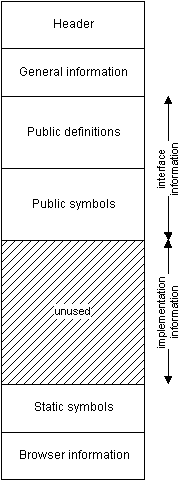
\epsfig{file=pics/ppu.png}
\else
\epsfig{file=pics/ppu.eps}
\fi
\end{center}
\end{figure}
\end{latexonly}

To read or write the ppufile, the ppu unit \file{ppu.pas} can be used,
which has an object called tppufile which holds all routines that deal
with ppufile handling. While describing the layout of a ppufile, the
methods which can be used for it are presented as well.

A unit file consists of basically five or six parts:
\begin{enumerate}
\item A unit header.
\item A general information part (wrongly named interface section in the code)
\item A definition part. Contains all type and procedure definitions.
\item A symbol part. Contains all symbol names and references to their
definitions.
\item A browser part. Contains all references from this unit to other
units and inside this unit. Only available when the \var{uf\_has\_browser} flag is
set in the unit flags
\item A file implementation part (currently unused).
\end{enumerate}

\section{reading ppufiles}

We will first create an object ppufile which will be used below. We are
opening unit \file{test.ppu} as an example.

\begin{verbatim}
var
  ppufile : pppufile;
begin
{ Initialize object }
  ppufile:=new(pppufile,init('test.ppu');
{ open the unit and read the header, returns false when it fails }
  if not ppufile.openfile then
    error('error opening unit test.ppu');

{ here we can read the unit }

{ close unit }
  ppufile.closefile;
{ release object }
  dispose(ppufile,done);
end;
\end{verbatim}

Note: When a function fails (for example not enough bytes left in an
entry) it sets the \var{ppufile.error} variable.

%%%%%%%%%%%%%%%%%%%%%%%%%%%%%%%%%%%%%%%%%%%%%%%%%
% The Header
\section{The Header}

The header consists of a record (\var{tppuheader}) containing
several pieces of information for recompilation. This is shown
in \seet{PPUHeader}. The header is always stored in little-endian
format.

\begin{FPCltable}{|l|c|l|}{PPU Header}{PPUHeader}
\hline
offset & size (bytes) & description \\
\hline
00h   &   3          &  Magic : 'PPU' in ASCII \\
03h   &   3          &  PPU File format version (e.g : '021' in ASCII) \\
06h   &   2          &  Compiler version used to compile this module (major,minor)\\
08h   &   2          &  Code module target processor  \\
0Ah   &   2          &  Code module target operating system \\
0Ch   &   4          &  Flags for PPU file  \\
10h   &   4          &  Size of PPU file (without header) \\
14h   &   4          &  CRC-32 of the entire PPU file \\
18h   &   4          &  CRC-32 of partial data of PPU file (public data mostly) \\
1Ch   &   8          &  Reserved \\
\hline
\end{FPCltable}

The header is already read by the \var{ppufile.openfile} command.
You can access all fields using \var{ppufile.header} which holds
the current header record.

\begin{FPCltable}{|ll|}{PPU CPU Field values}{PPUHeaderCPU}
\hline
value & description \\
\hline
0     & unknown \\
1     & Intel 80x86 or compatible \\
2     & Motorola 680x0 or compatible \\
3     & Alpha AXP or compatible \\
4     & PowerPC or compatible \\
\hline
\end{FPCltable}

Some of the possible flags in the header, are described in \seet{PPUHeaderFlags}.
Not all the flags are described, for more information, read the source code of
\file{ppu.pas}.

\begin{FPCltable}{|ll|}{PPU Header Flag values}{PPUHeaderFlags}
\hline
Symbolic bit flag name & Description\\
\hline
uf\_init & Module has an initialization (either Delphi or TP style) section. \\
uf\_finalize & Module has a finalization section. \\
uf\_big\_endian & All the data stored in the chunks is in big-endian format.\\
uf\_has\_browser & Unit contains symbol browser information. \\
uf\_smart\_linked & The code module has been smartlinked.\\
uf\_static\_linked & The code is statically linked. \\
uf\_has\_resources & Unit has resource section. \\
\hline
\end{FPCltable}


%%%%%%%%%%%%%%%%%%%%%%%%%%%%%%%%%%%%%%%%%%%%%5
% The sections
\section{The sections}

Apart from the header section, all the data in the PPU file is separated
into data blocks, which permit easily adding additional data blocks,
without compromising backward compatibility. This is similar to both
Electronic Arts IFF chunk format and Microsoft's RIFF chunk format.

Each 'chunk' (\var{tppuentry}) has the following format, and can be
nested:

\begin{FPCltable}{|l|c|l|}{chunk data format}{ChunkFormats}
\hline
offset & size (bytes) & description \\
\hline
00h   &   1          &  Block type (nested (2) or main (1)) \\
01h   &   1          &  Block identifier \\
02h   &   4          &  Size of this data block \\
06h+  &   <variable> &  Data for this block \\
\hline
\end{FPCltable}


Each main section chunk must end with an end chunk. Nested chunks
are used for record, class or object fields.


To read an entry you can simply call \var{ppufile.readentry:byte},
it returns the
\var{tppuentry.nr} field, which holds the type of the entry.
A common way how this works is (example is for the symbols):

\begin{verbatim}
  repeat
    b:=ppufile.readentry;
    case b of
   ib<etc> : begin
             end;
 ibendsyms : break;
    end;
  until false;
\end{verbatim}

The possible entry types are found in \file{ppu.pas}, but a short
description of the most common ones are shown in \seet{PPUEntryTypes}.

\begin{FPCltable}{|lll|}{Possible PPU Entry types}{PPUEntryTypes}
\hline
Symbolic name & Location & Description\\
\hline
ibmodulename  & General & Name of this unit.\\
ibsourcefiles & General & Name of source files.\\
ibusedmacros & General & Name and state of macros used.\\
ibloadunit  & General & Modules used by this units. \\
inlinkunitofiles & General & Object files associated with this unit. \\
iblinkunitstaticlibs & General & Static libraries associated with this unit. \\
iblinkunitsharedlibs & General & Shared libraries associated with this unit. \\
ibendinterface & General & End of General information section. \\
ibstartdefs & Interface & Start of definitions. \\
ibenddefs & Interface & End of definitions. \\
ibstartsyms  & Interface & Start of symbol data. \\
ibendsyms & Interface  & End of symbol data. \\
ibendimplementation & Implementation & End of implementation data. \\
ibendbrowser & Browser & End of browser section. \\
ibend & General & End of Unit file. \\
\hline
\end{FPCltable}


Then you can parse each entry type yourself. \var{ppufile.readentry} will take
care of skipping unread bytes in the entry and reads the next entry
correctly! A special function is \var{skipuntilentry(untilb:byte):boolean;}
which will read the ppufile until it finds entry \var{untilb} in the main
entries.

Parsing an entry can be done with \var{ppufile.getxxx} functions. The
available functions are:
\begin{verbatim}
procedure ppufile.getdata(var b;len:longint);
function  getbyte:byte;
function  getword:word;
function  getlongint:longint;
function  getreal:ppureal;
function  getstring:string;
\end{verbatim}

To check if you're at the end of an entry you can use the following
function:

\begin{verbatim}
function  EndOfEntry:boolean;
\end{verbatim}
{\em notes:}
\begin{enumerate}
\item \var{ppureal} is the best real that exists for the cpu where the
unit is created for. Currently it is \var{extended} for i386 and
\var{single} for m68k.
\item the \var{ibobjectdef} and \var{ibrecorddef} have stored a definition
and symbol section for themselves. So you'll need a recursive call. See
\file{ppudump.pp} for a correct implementation.
\end{enumerate}

A complete list of entries and what their fields contain can be found
in \file{ppudump.pp}.

\section{Creating ppufiles}
Creating a new ppufile works almost the same as reading one.
First you need to init the object and call create:
\begin{verbatim}
  ppufile:=new(pppufile,init('output.ppu'));
  ppufile.createfile;
\end{verbatim}

After that you can simply write all needed entries. You'll have to take
care that you write at least the basic entries for the sections:
\begin{verbatim}
  ibendinterface
  ibenddefs
  ibendsyms
  ibendbrowser (only when you've set uf_has_browser!)
  ibendimplementation
  ibend
\end{verbatim}

Writing an entry is a little different than reading it. You need to first
put everything in the entry with ppufile.putxxx:
\begin{verbatim}
procedure putdata(var b;len:longint);
procedure putbyte(b:byte);
procedure putword(w:word);
procedure putlongint(l:longint);
procedure putreal(d:ppureal);
procedure putstring(s:string);
\end{verbatim}

After putting all the things in the entry you need to call
\var{ppufile.writeentry(ibnr:byte)} where \var{ibnr} is the entry number
you're writing.

At the end of the file you need to call \var{ppufile.writeheader} to write the
new header to the file. This takes automatically care of the new size of the
ppufile. When that is also done you can call \var{ppufile.closefile} and dispose the
object.

Extra functions/variables available for writing are:
\begin{verbatim}
ppufile.NewHeader;
ppufile.NewEntry;
\end{verbatim}
This will give you a clean header or entry. Normally this is called
automatically in \var{ppufile.writeentry}, so there should be no need to
call these methods.
\begin{verbatim}
ppufile.flush;
\end{verbatim}

to flush the current buffers to the disk
\begin{verbatim}
ppufile.do_crc:boolean;
\end{verbatim}
set to false if you don't want that the crc is updated, this is necessary
if you write for example the browser data.

%%%%%%%%%%%%%%%%%%%%%%%%%%%%%%%%%%%%%%%%%%%%%%%%%%%%%%%%%%%%%%%%%%%%%
% Appendix B
%%%%%%%%%%%%%%%%%%%%%%%%%%%%%%%%%%%%%%%%%%%%%%%%%%%%%%%%%%%%%%%%%%%%%

\chapter{Compiler and RTL source tree structure}
\label{ch:AppB}

%%%%%%%%%%%%%%%%%%%%%%%%%%%%%%%%%%%%%%%%%%%%%%%%%
% The compiler source tree
\section{The compiler source tree}

All compiler source files are in several directories, normally the
non-processor specific parts are in \file{source/compiler}. Subdirectories
are present for each of the supported processors and target operating systems.

For more informations about the structure of the compiler have a look at the
Compiler Manual which contains also some informations about
compiler internals.

The \file{compiler} directory also contains a subdirectory \var{utils},
which contains mainly the utilities for creation and maintainance of the
message files.

%%%%%%%%%%%%%%%%%%%%%%%%%%%%%%%%%%%%%%%%%%%%%%%%%
% The RTL source tree
\section{The RTL source tree}
The RTL source tree is divided in many subdirectories, but is very
structured and easy to understand. It mainly consists of three parts:

\begin{enumerate}
\item A OS-dependent directory. This contains the files that are different for
each operating system. When compiling the RTL, you should do it here. The
following directories exist:
\begin{itemize}
\item \file{atari} for the \atari.
\item \file{amiga} for the \amiga.
\item \file{beos}  for \beos. It has one subdirectory for each of the
supported processors.
\item \file{freebsd} for the \freebsd platform.
\item \file{go32v1} For \dos, using the GO32v1 extender. Not maintained any
more.
\item \file{go32v2} For \dos, using the GO32v2 extender.
\item \file{linux} for \linux platforms. It has one subdirectory for each of the supported
processors.
\item \file{netbsd} for \netbsd platforms. It has one subdirectory for each of the supported
processors.
\item \file{palmos} for the \palmos Dragonball processor based platform.
\item \file{os2} for \ostwo.
\item \file{sunos} for the \solaris platform. It has one subdirectory for each of the supported
processors.
\item \file{qnx} for the \qnx.
\item \file{win32} for Win32 platforms.
\item \file{posix} for posix interfaces (used for easier porting).
\item \file{unix} for unix common interfaces (used for easier porting).
\end{itemize}
\item A processor dependent directory. This contains files that are system
independent, but processor dependent. It contains mostly optimized routines
for a specific processor. The following directories exist:
\begin{itemize}
\item \file{i386} for the Intel 80x86 series of processors.
\item \file{m68k} for the Motorola 680x0 series of processors.
\end{itemize}
\item An OS-independent and Processor independent directory: \file{inc}. This
contains complete units, and include files containing interface parts of
units as well as generic versions of processor specific routines.
\end{enumerate}

%%%%%%%%%%%%%%%%%%%%%%%%%%%%%%%%%%%%%%%%%%%%%%%%%%%%%%%%%%%%%%%%%%%%%
% Appendix C
%%%%%%%%%%%%%%%%%%%%%%%%%%%%%%%%%%%%%%%%%%%%%%%%%%%%%%%%%%%%%%%%%%%%%

\chapter{Compiler limits}
\label{ch:AppC}
Although many of the restrictions imposed by the MS-DOS system are removed
by use of an extender, or use of another operating system, there still are
some limitations to the compiler:
\begin{enumerate}
\item Procedure or Function definitions can be nested to a level of 32.
\item Maximally 255 units can be used in a program when using the real-mode
compiler (i.e. a binary that was compiled by Borland Pascal). When using the 32-bit compiler, the limit is set to 1024. You can
change this by redefining the \var{maxunits} constant in the
\file{files.pas} compiler source file.
\end{enumerate}

%%%%%%%%%%%%%%%%%%%%%%%%%%%%%%%%%%%%%%%%%%%%%%%%%%%%%%%%%%%%%%%%%%%%%
% Appendix D
%%%%%%%%%%%%%%%%%%%%%%%%%%%%%%%%%%%%%%%%%%%%%%%%%%%%%%%%%%%%%%%%%%%%%
\chapter{Compiler modes}
\label{ch:AppD}

Here we list the exact effect of the different compiler modes. They can be
set with the \var{\$Mode} switch, or by command line switches.

\section{FPC mode}
This mode is selected by the \var{{\$MODE FPC}} switch. On the command-line,
this means that you use none of the other compatibility mode switches.
It is the default mode of the compiler. This means essentially:
\begin{enumerate}
\item You must use the address operator to assign procedural variables.
\item A forward declaration must be repeated exactly the same by the
implementation of a function/procedure. In particular, you can not omit the
parameters when implementing the function or procedure.
\item Overloading of functions is allowed.
\item Nested comments are allowed.
\item The Objpas unit is NOT loaded.
\item You can use the cvar type.
\item PChars are converted to strings automatically.
\end{enumerate}
\section{TP mode}
This mode is selected by the \var{{\$MODE TP}} switch. On the command-line,
this mode is selected by the \var{-So} switch.

\begin{enumerate}
\item Enumeration sizes default to a storage size of 1 byte if there
are less than 257 elements.
\item You cannot use the address operator to assign procedural variables.
\item A forward declaration must not be repeated exactly the same by the
implementation of a function/procedure. In particular, you can omit the
parameters when implementing the function or procedure.
\item Overloading of functions is not allowed.
\item The Objpas unit is NOT loaded.
\item Nested comments are not allowed.
\item You can not use the cvar type.
\end{enumerate}
\section{Delphi mode}
This mode is selected by the \var{{\$MODE DELPHI}} switch. On the command-line,
this mode is selected by the \var{-Sd} switch.
\begin{enumerate}
\item You can not use the address operator to assign procedural variables.
\item A forward declaration must not be repeated exactly the same by the
implementation of a function/procedure. In particular, you not omit the
parameters when implementing the function or procedure.
\item Overloading of functions is not allowed.
\item Nested comments are not  allowed.
\item The Objpas unit is loaded right after the \file{system} unit. One of the
consequences of this is that the type \var{Integer} is redefined as
\var{Longint}.
\end{enumerate}
\section{GPC mode}
This mode is selected by the \var{{\$MODE GPC}} switch. On the command-line,
this mode is selected by the \var{-Sp} switch.
\begin{enumerate}
\item You must use the address operator to assign procedural variables.
\item A forward declaration must not be repeated exactly the same by the
implementation of a function/procedure. In particular, you can omit the
parameters when implementing the function or procedure.
\item Overloading of functions is not allowed.
\item The Objpas unit is NOT loaded.
\item Nested comments are not allowed.
\item You can not use the cvar type.
\end{enumerate}
\section{OBJFPC mode}
This mode is selected by the \var{{\$MODE OBJFPC}} switch. On the command-line,
this mode is selected by the \var{-S2} switch.
\begin{enumerate}
\item You must use the address operator to assign procedural variables.
\item A forward declaration must be repeated exactly the same by the
implementation of a function/procedure. In particular, you can not omit the
parameters when implementing the function or procedure.
\item Overloading of functions is allowed.
\item Nested comments are allowed.
\item The Objpas unit is loaded right after the \file{system} unit. One of the
consequences of this is that the type \var{Integer} is redefined as
\var{Longint}.
\item You can use the cvar type.
\item PChars are converted to strings automatically.
\end{enumerate}

%%%%%%%%%%%%%%%%%%%%%%%%%%%%%%%%%%%%%%%%%%%%%%%%%%%%%%%%%%%%%%%%%%%%%
% Appendix E
%%%%%%%%%%%%%%%%%%%%%%%%%%%%%%%%%%%%%%%%%%%%%%%%%%%%%%%%%%%%%%%%%%%%%

\chapter{Using \file{fpcmake}}
\label{ch:makefile}
\newcommand{\mvar}[1]{\var{\$(#1)}}
\newcommand{\fpcmake}{\file{fpcmake}}
\section{Introduction}
\fpc comes with a special makefile tool, \fpcmake{}, which can be
used to construct a \file{Makefile} for use with \gnu \file{make}.
All sources from the \fpc team are compiled with this system.

\fpcmake{} uses a file \file{Makefile.fpc} and constructs a file
\file{Makefile} from it, based on the settings in \file{Makefile.fpc}.

The following sections explain what settings can be set in \file{Makefile.fpc},
what variables are set by \var{fpcmake}, what variables it expects to be set,
and what targets it defines. After that, some settings in the resulting
\file{Makefile} are explained.

\section{Functionality}
\label{se:fpcmakefunctionality}
\file{fpcmake} generates a makefile, suitable for GNU \file{make}, 
which can be used to 
\begin{enumerate}
\item Compile units and programs, fit for testing or for final distribution.
\item Compile example units and programs separately.
\item Install compiled units and programs in standard locations.
\item Make archives for distribution of the generated programs and units.
\item Clean up after compilation and tests.
\end{enumerate}
\file{fpcmake} knows how the \fpc compiler operates, which command line
options it uses, how it searches for files and so on; It uses this knowledge
to construct sensible command-lines. 

Specifically, it constructs the following targets in the final makefile:
\begin{description}
\item[all] Makes all units and programs.
\item[debug] Makes all units and programs with debug info included.
\item[smart] Makes all units and programs in smartlinked version.
\item[examples] Makes all example units and programs.
\item[shared] Makes all units and programs in shared library version
(currently disabled)
\item[install] Installs all units and programs.
\item[sourceinstall] Installs the sources to the \fpc source tree.
\item[exampleinstall] Installs any example programs and units.
\item[distinstall] Installs all units and programs, as well as example units
and programs.
\item[zipinstall] Makes an archive of the programs and units which can be
used to install them on another location, i.e. it makes an archive that can
be used to distribute the units and programs.
\item[zipsourceinstall] Makes an archive of the program and unit sources
which can be used to distribute the sources.
\item[zipexampleinstall] Makes an archive of the example programs and units 
which can be used to install them on another location, i.e. it makes an 
archive that can be used to distribute the example units and programs.
\item[zipdistinstall] Makes an archive of both the normal as well as the
example programs and units. This archive can be used to install them on 
another location, i.e. it makes an archive that can be used to 
distribute.
\item[clean] Cleans all files that are produced by a compilation.
\item[distclean] Cleans all files that are produced by a compilation, as
well as any archives, examples or files left by examples.
\item[cleanall] Same as clean.
\item[info] Produces some information on the screen about used programs,
file and directory locations, where things will go when installing and so
on.
\end{description}
Each of these targets can be highly configured, or even totally overridden
by the configuration file \file{Makefile.fpc}

\section{Usage}
\file {fpcmake} reads a \file{Makefile.fpc} and converts it to a
\file{Makefile} suitable for reading by \gnu \file{make}
to compile your projects. It is similar in functionality to GNU
\file{configure} or \file{Imake} for making X projects.

\fpcmake{} accepts filenames of makefile description files
as its command-line arguments. For each of these files it will
create a \file{Makefile} in the same directory where the file is
located, overwriting any existing file with that name.

If no options are given, it just attempts to read the file
\file{Makefile.fpc} in the current directory and tries to
construct a \file{Makefile} from it if the \var{-m} option is
given. Any previously existing \file{Makefile} will be erased.

if the \var{-p} option is given, instead of a \file{Makefile}, a
\var{Package.fpc} is generated. A \file{Package.fpc} file describes the
package and it's dependencies on other packages.

Additionally, the following command-line options are recognized:
\begin{description}
\item[-p] A \file{Package.fpc} file is generated.
\item[-w] A \file{Makefile} is generated.
\item[-T targets] Support only specified target systems. \var{Targets} is a
comma-separated list of targets. Only rule for the specified targets
will be written.
\item[-v] Be more verbose.
\item[-q] be quiet.
\item[-h] Writes a small help message to the screen.
\end{description}

% Makefile.fpc format.
\section{Format of the configuration file}
This section describes the rules that can be present in the file
that is fed to \fpcmake{}.

The file \file{Makefile.fpc} is a plain ASCII file that contains
a number of pre-defined sections as in a \windows \file{.ini}-file,
or a Samba configuration file.

They look more or less as follows:
\begin{verbatim}
[package]
name=mysql
version=1.0.5

[target]
units=mysql_com mysql_version mysql
examples=testdb

[require]
libc=y

[install]
fpcpackage=y

[default]
fpcdir=../..
\end{verbatim}

The following sections are recognized (in alphabetical order):

\subsection{clean}
Specifies rules for cleaning the directory of units and programs.
The following entries are recognized:
\begin{description}
\item[units] names of all units that should be removed when cleaning.
Don't specify extensions, the makefile will append these by itself.
\item[files] names of files that should be removed. Specify full filenames.
\end{description}

\subsection{compiler}
In this section values for various compiler options can be specified, 
such as the location of several directories and search paths.

The following general keywords are recognised:
\begin{description}
\item[options] The value of this key will be passed on to the compiler as
options.
\item[version] If a specific or minimum compiler version is needed to
compile the units or programs, then this version should be specified here.
\end{description}

The following keys can be used to control the location of the various
directories used by the compiler:
\begin{description}
\item[unitdir]
A colon-separated list of directories that must be added to the unit
search path of the compiler.
\item[librarydir]
A colon-separated list of directories that must be added to the library
search path of the compiler.
\item[objectdir]
A colon-separated list of directories that must be added to the object file
search path of the compiler.
\item[targetdir]
Specifies the directory where the compiled programs should go.
\item[sourcedir]
A space separated list of directories where sources can reside.
This will be used for the \var{vpath} setting of \gnu \file{make}.
\item[unittargetdir]
Specifies the directory where the compiled units should go.
\item[includedir]
A colon-separated list of directories that must be added to the include file
search path of the compiler.
\item[sourcedir]
\end{description}


\subsection{Default}
The \var{default} section contains some default settings. The following keywords
are recognized:
\begin{description}
\item[cpu]
Specifies the default target processor for which the \file{Makefile}
should compile the units and programs. By default this is determined from
the default compiler processor.
\item[dir]
Specifies any subdirectories that make should also descend in and
make the specified target there as well.
\item[fpcdir]
Specifies the directory where all the \fpc source trees reside. Below this
directory the \file{Makefile} expects to find the \file{rtl}, \file{fcl} and
\file{packages} directory trees.
\item[rule] Specifies the default rule to execute. \fpcmake{}
will make sure that this rule is executed if make is executed without
arguments, i.e., without an explicit target.
\item[target]
Specifies the default operating system target for which the \file{Makefile}
should compile the units and programs. By default this is determined from
the default compiler target.
\end{description}

\subsection{Dist}
The \var{Dist} section controls the generation of a distribution package. 
A distribution package is a set of archive files (zip files or tar files 
on unix systems) that can be used to distribute the package.

The following keys can be placed in this section:
\begin{description}
\item[destdir] Specifies the directory where the generated zip files should
be placed.
\item[zipname] Name of the archive file to be created. If no zipname is
specified, this defaults to the package name.
\item[ziptarget] This is the target that should be executed before the
archive file is made. This defaults to \var{install}.
\end{description}

\subsection{Install}
Contains instructions for installation of the compiler units and programs. The
following keywords are recognized:
\begin{description}
\item[basedir]
The directory that is used as the base directory for the installation of
units. Default this is \var{prefix} appended with \var{/lib/fpc/FPC\_VERSION}
for \linux or simply the \var{prefix} on other platforms.
\item[datadir] Directory where data files will be installed, i.e. the files
specified with the \var{Files} keyword.
\item[fpcpackage] A boolean key. If this key is specified and equals \var{y}, 
the files will be installed as a fpc package under the \fpc units directory,
i.e. under a separate directory. The directory will be named with the name 
specified in the \var{package} section.
\item[files] extra data files to be installed in the directory specified
with the \var{datadir} key.
\item[prefix] is the directory below wchich all installs are done.
This corresponds to the \var{--prefix} argument to \gnu \file{configure}.
It is used for the installation of programs and units. By default, this is
\file{/usr} on \linux, and \file{/pp} on all other platforms.
\item[units] extra units that should be installed, and which are not part of
the unit targets. The units in the units target will be installed
automatically.
\end{description}
Units will be installed in the subdirectory  \file{units/\$(OS\_TARGET)}
of the \var{dirbase} entry.

\subsection{Package}
If a package (i.e. a collection of units that work together) is being 
compiled, then this section is used to keep package information. 
The following information can be stored:
\begin{description}
\item[name] The name of the package. When installing it under the package
directory, this name will be used to create a directory (unless it is
overridden by one of the installation options)
\item[version] The version of this package.
\item[main] If the package is part of another package, this key can be
specified to indicate which package it is part of.
\end{description}

\subsection{Prerules}
Anything that is in this section will be inserted as-is in the makefile
\textit{before} the makefile target rules that are generated by fpcmake.
This means that any variables that are normally defined by fpcmake rules
should not be used in this section.

\subsection{Requires}
This section is used to indicate dependency on external packages (i.e units)
or tools. The following keywords can be used:
\begin{description}
\item[fpcmake] Minimal version of fpcmake that this \file{makefile.fpc} needs.
\item[packages] Other packages that should be compiled before this package
can be compiled. Note that this will also add all packages these packages
depend on to the dependencies of this package. By default, the \fpc Run-Time
Library is added to this list.
\item[libc] a boolean value that indicates whether this package needs the C
library.
\item[nortl] a boolean that prevents the addition of the \fpc Run-Time 
Library to the required packages.
\item[unitdir] These directories will be added to the units search path of
the compiler.
\item[packagedir] List of package directories. The packages in these
directories will be made as well before making the current package.
\item[tools] A list of executables of extra tools that are required. The
full path to these tools will be defined in the makefile as a variable with
the same name as the tool name, only in uppercase. For example, the
following definition:
\begin{verbatim}
tools=upx
\end{verbatim}
will lead to the definition of a variable with the name \var{UPX} which will
contain the full path to the \file{upx} executable.
\end{description}

\subsection{Rules}
In this section dependency rules for the units and any other needed 
targets can be inserted. It will be included at the end of the generated
makefile. Targets or 'default rules' that are defined by \fpcmake{} 
can be inserted here; if they are not present, then \fpcmake{} will generate
a rule that will call the generic \var{fpc\_} version. For a list of standard 
targets that will be defined by \fpcmake{}, see \sees{fpcmakefunctionality}.

For example, it is possible to define a target \var{all:}. If it is not
defined, then \fpcmake{} will generate one which simply calls
\var{fpc\_all}:
\begin{verbatim}
all: fpc_all
\end{verbatim}
The \var{fpc\_all} rule will make all targets as defined in the \var{Target}
section.

\subsection{Target}
This is the most important section of the \file{makefile.fpc} file. Here the
files are defined which should be compiled when the 'all' target is
executed. 

The following keywords can be used there:
\begin{description}
\item[dirs]
A space separated list of directories where make should also be run.
\item[exampledirs] 
A space separated list of directories with example programs. The examples
target will descend in this list of directories as well.
\item[examples]
A space separated list of example programs that need to be compiled when
the user asks to compile the examples. Do not specify an extension,
the extension will be appended.
\item[loaders]
A space separated list of names of assembler files that must be assembled.
Don't specify the extension, the extension will be appended.
\item[programs]
A space separated list of program names that need to be compiled. Do not
specify an extension, the extension will be appended.
\item[rsts] a list of \file{rst} files that needs to be converted to \file{.po}
files for use with \gnu \file{gettext} and internationalization routines.
\item[units]
A space separated list of unit names that need to be compiled. Do not
specify an extension, just the name of the unit as it would appear un a
\var{uses} clause is sufficient.
\end{description}

\section{Programs needed to use the generated makefile}
At least the following programs are needed by the generated \file{Makefile}
to function correctly:
\begin{description}
\item[cp] a copy program.
\item[date] a program that prints the date.
\item[install] a program to install files.
\item[make] the \file{make} program, obviously.
\item[pwd] a program that prints the current working directory.
\item[rm] a program to delete files.
\item[zip] the zip archiver program. (on dos/windows/OS2 systems only)
\item[tar] the tar archiver program (on Unix systems only).
\end{description}
These are standard programs on \linux systems, with the possible exception of
\file{make}. For \dos or \windowsnt, they can be found in the
file \file{makeutil.zip} on the \fpc FTP site.

The following programs are optionally needed if you use some special targets.
Which ones you need are controlled by the settings in the \var{tools} section.
\begin{description}
\item[cmp] a \dos and \windowsnt file comparer. 
\item[diff] a file comparer. 
\item[ppdep] the ppdep depency lister. Distributed with \fpc.
\item[ppufiles] the ppufiles unit file dependency lister. Distributed with \fpc.
\item[ppumove] the \fpc unit mover. 
\item[sed] the \file{sed} program. 
\item[upx] the UPX executable packer. 
\end{description}
All of these can also be found on the \fpc FTP site for \dos and \windowsnt.
\file{ppdep,ppufiles} and \file{ppumove} are distributed with the \fpc
compiler.

%
\section{Variables that affect the generated makefile}
The makefile generated by \fpcmake{} contains a lot of variables.
Some of them are set in the makefile itself, others can be set and are taken
into account when set.

These variables can be split in two groups:
\begin{itemize}
\item Directory variables.
\item Compiler command-line variables.
\end{itemize}
Each group will be discussed separately.

\subsection{Directory variables}

The first set of variables controls the directories that are
recognised in the makefile. They should not be set in the
\file{Makefile.fpc} file, but can be specified on the commandline.
\begin{description}
\item[INCDIR] this is a list of directories, separated by spaces, that will
be added as include directories to the compiler command-line.  Each
directory in the list is prepended with \var{-I} and added to the
compiler options.
\item[UNITDIR] this is a list of directories, separated by spaces, that will
be added as unit search directories to the compiler command-line.  Each
directory in the list is prepended with \var{-Fu} and added to the
compiler options.
\item[LIBDIR] is a list of library paths, separated by spaces. Each
directory in the list is prepended with \var{-Fl} and added to the
compiler options.
\item[OBJDIR] is a list of object file directories, separated by spaces, that is
added to the object files path, i.e. Each directory in the list is prepended with
\var{-Fo}.
\end{description}

\subsection{Compiler command-line variables }
The following variable can be set on the \file{make} command-line,
they will be recognised and integrated in the compiler command-line options.:

\begin{description}
\item[CREATESMART] If this variable is defined, it tells the compiler to 
create smartlinked units. Adds \var{-CX} to the command-line options.
\item[DEBUG] If defined, this will cause the compiler to include debug information in
the generated units and programs. It adds \var{-gl} to the compiler
command-line, and will define the \var{DEBUG} define.
\item[LINKSMART] Defining this variable tells the compiler to use smartlinking. 
It adds \var{-XX} to the compiler command-line options.
\item[OPT] Any options that you want to pass to the compiler. The contents
of \var{OPT} is simply added to the compiler command-line.
\item[OPTDEF] Are optional defines, added to the command-line of the
compiler. They get \var{-d} prepended to them.
\item[OPTIMIZE] if this variable is defined, this will add \var{-OG2p3} to
the command-line options.
\item[RELEASE] if this variable is defined, this will add the \var{-Xs -OG2p3 -n} 
options to the command-line options, and will define the \var{RELEASE} define.
\item[STRIP] if this variable is defined, this will add the \var{-Xs} option 
to the command-line options.
\item[VERBOSE] if this variable is defined, then \var{-vnwi} will be added
to the command-line options.
\end{description}

\section{Variables set by \fpcmake{}}

The makefile generated by \fpcmake{} contains a lot of makefile variables.
\fpcmake{} will write all of the keys in the \file{makefile.fpc} as
makefile variables in the form \var{SECTION\_KEYNAME}. This means that the
following section:
\begin{verbatim}
[package]
name=mysql
version=1.0.5
\end{verbatim}
will result in the following variable definitions:
\begin{verbatim}
override PACKAGE_NAME=mysql
override PACKAGE_VERSION=1.0.5
\end{verbatim}

Most targets and rules are constructed using these variables. They will be
listed below, together with other variables that are defined by \fpcmake{}.

The following sets of variables are defined:
\begin{itemize}
\item Directory variables.
\item Program names.
\item File extensions.
\item Target files.
\end{itemize}
Each of these sets is discussed in the subsequent:

\subsection{Directory variables}

The following compiler directories are defined by the makefile:

\begin{description}
\item[BASEDIR] is set to the current directory if the \file{pwd} command is
available. If not, it is set to '.'.

\item[COMPILER\_INCDIR] is a space-separated list of library paths. Each
directory in the list is prepended with \var{-Fl} and added to the
compiler options. Set by the \var{incdir} keyword in the \var{Compiler} section.

\item[COMPILER\_LIBDIR] is a space-separated list of library paths. Each
directory in the list is prepended with \var{-Fl} and added to the 
compiler options. Set by the \var{libdir} keyword in the \var{Compiler} section.

\item[COMPILER\_OBJDIR] is a list of object file directories, separated by
 spaces. Each directory in the list is prepended with \var{-Fo} and
added to the compiler options.
Set by the \var{objdir} keyword in the \var{Compiler} section.

\item[COMPILER\_TARGETDIR] This directory is added as the output directory of
the compiler, where all units and executables are written, i.e. it gets
\var{-FE} prepended. It is set by the \var{targtdir} keyword in the
\var{Compiler} section.

\item[COMPILER\_TARGETUNITDIR] If set, this directory is added as the output directory of
the compiler, where all units and executables are written, i.e. it gets
\var{-FU} prepended.It is set by the \var{targtdir} keyword in the
\var{Dirs} section.

\item[COMPILER\_UNITDIR] is a list of unit directories, separated by spaces.
Each directory in the list is prepended with \var{-Fu} and is added to the
compiler options.
Set by the \var{unitdir} keyword in the \var{Compiler} section.

\item[GCCLIBDIR] (\linux only) is set to the directory where \file{libgcc.a}
is. If \var{needgcclib} is set to \var{True} in the \var{Libs} section, then
this directory is added to the compiler commandline with \var{-Fl}.

\item[OTHERLIBDIR] is a space-separated list of library paths. Each
directory in the list is prepended with \var{-Fl} and added to the 
compiler options.  If it is not defined on linux, then the contents of 
the \file{/etc/ld.so.conf} file is added.
\end{description}

The following directories are used for installs:
\begin{description}
\item[INSTALL\_BASEDIR] is the base for all directories where units are
installed. By default, On \linux, this is set to 
\mvar{INSTALL\_PREFIX}\var{/lib/fpc/}\mvar{RELEASEVER}.\\ On other systems,
it is set to \mvar{PREFIXINSTALLDIR}. You can also set it with the
\var{basedir} variable in the \var{Install} section.

\item[INSTALL\_BINDIR] is set to \mvar{INSTALL\_BASEDIR}/\var{bin} on \linux,
and\\ \mvar{INSTALL\_BASEDIR}/\var{bin}/\mvar{OS\_TARGET} on other systems.
This is the place where binaries are installed.

\item[INSTALL\_DATADIR] The directory where data files are installed. Set by
the \var{Data} key in the \var{Install} section.

\item[INSTALL\_LIBDIR] is set to \mvar{INSTALL\_PREFIX}/lib on \linux,\\
 and \mvar{INSTALL\_UNITDIR} on other systems.

\item[INSTALL\_PREFIX] is set to \file{/usr/local} on \linux, \file{/pp} on \dos
or \windowsnt. Set by the \var{prefix} keyword in the \var{Install}
section.

\item[INSTALL\_UNITDIR] is where units will be installed. This is set to\\
\mvar{INSTALL\_BASEDIR}/units/\mvar{OS\_TARGET}. If the units are compiled
as a package, \mvar{PACKAGE\_NAME} is added to the directory.
\end{description}

\subsection{Target variables}

The second set of variables controls the targets that are constructed
by the makefile. They are created by \fpcmake{}, so you can use
them in your rules, but you shouldn't assign values to them yourself.

\begin{description}
\item[TARGET\_DIRS] This is the list of directories that make will descend
into when compiling. Set by the \var{Dirs} key in the \var{Target} section?

\item[TARGET\_EXAMPLES] The list of examples programs that must be compiled.
Set by the \var{examples} key in the \var{Target} section.

\item[TARGET\_EXAMPLEDIRS] the list of directories that make will descend
into when compiling examples. Set by the \var{exampledirs} key in the 
\var{Target} section.

\item[TARGET\_LOADERS] is a list of space-separated names that identify
loaders to be compiled. This is mainly used in the compiler's RTL sources.
It is set by the \var{loaders} keyword in the \var{Targets} section.

\item[TARGET\_PROGRAMS] This is a list of executable names that will be compiled.
the makefile appends \mvar{EXEEXT} to these names. It is set by the
\var{programs} keyword in the \var{Target} section.

\item[TARGET\_UNITS] This is a list of unit names that will be compiled. The
makefile appends \mvar{PPUEXT} to each of these names to form the unit file
name. The sourcename is formed by adding \mvar{PASEXT}.
It is set by the \var{units} keyword in the \var{Target} section.

\item[ZIPNAME] is the name of the archive that will be created by the
makefile.
It is set by the \var{zipname} keyword in the \var{Zip} section.

\item[ZIPTARGET] is the target that is built before the archive is made.
this target is built first. If successful, the zip archive will be made.
It is set by the \var{ziptarget} keyword in the \var{Zip} section.

\end{description}

\subsection{Compiler command-line variables}

The following variables control the compiler command-line:
\begin{description}

\item[CPU\_SOURCE] the target CPU type is added as a define to the compiler
command line. This is determined by the Makefile itself.

\item[CPU\_TARGET] the target CPU type is added as a define to the compiler
command line. This is determined by the Makefile itself.

\item[OS\_SOURCE] What platform the makefile is used on. Detected
automatically.

\item[OS\_TARGET] What platform will be compiled for. Added to the
compiler command-line with a \var{-T} prepended.
\end{description}


\subsection{Program names}

The following variables are program names, used in makefile targets.
\begin{description}
\item[AS] The assembler. Default set to \file{as}.
\item[COPY] a file copy program. Default set to \file{cp -fp}.
\item[COPYTREE] a directory tree copy program. Default set to \file{cp -frp}.
\item[CMP] a program to compare files. Default set to \var{cmp}.
\item[DEL] a file removal program. Default set to \file{rm -f}.
\item[DELTREE] a directory removal program. Default set to \file{rm -rf}.
\item[DATE] a program to display the date.
\item[DIFF] a program to produce diff files.
\item[ECHO] an echo program.
\item[FPC] the Free Pascal compiler executable. Default set to
\var{ppc386.exe}
\item[INSTALL] a program to install files. Default set to \file{install -m
644} on \linux.
\item[INSTALLEXE] a program to install executable files. Default set to \file{install -m
755} on \linux.
\item[LD] The linker. Default set to \file{ld}.
\item[LDCONFIG] (\linux only) the program used to update the loader cache.
\item[MKDIR] a program to create directories if they don't exist yet. Default
set to \file{install -m 755 -d}
\item[MOVE] a file move program. Default set to \file{mv -f}
\item[PP] the Free Pascal compiler executable. Default set to
\var{ppc386.exe}
\item[PPAS] the name of the shell script created by the compiler if the
\var{-s} option is specified. This command will be executed after
compilation, if the \var{-s} option was detected among the options.
\item[PPUMOVE] the program to move units into one big unit library.
\item[PWD] the pwd program.
\item[SED] a stream-line editor program. Default set to \file{sed}.
\item[UPX] an executable packer to compress your executables into
self-extracting compressed executables.
\item[ZIPPROG] a zip program to compress files. zip targets are made with
this program
\end{description}

\subsection{File extensions}

The following variables denote extensions of files. These variables include
the \var{.} (dot) of the extension. They are appended to object names.

\begin{description}
\item[ASMEXT] is the extension of assembler files produced by the compiler.
\item[LOADEREXT] is the extension of the assembler files that make up the
executable startup code.
\item[OEXT] is the extension of the  object files that the compiler creates.
\item[PACKAGESUFFIX] is a suffix that is appended to package names in zip
targets. This serves so packages can be made for different OSes.
\item[PPLEXT] is the extension of shared library unit files.
\item[PPUEXT] is the extension of default units.
\item[RSTEXT] is the extension of the \file{.rst} resource string files.
\item[SHAREDLIBEXT] is the extension of shared libraries.
\item[SMARTEXT] is the extension of smartlinked unit assembler files.
\item[STATICLIBEXT] is the extension of static libraries.
\end{description}

\subsection{Target files}

The following variables are defined to make targets and rules easier:
\begin{description}
\item[COMPILER] is the complete compiler commandline, with all options
added, after all \file{Makefile} variables have been examined.
\item[DATESTR] contains the date.
\item[UNITPPUFILES] a list of unit files that will be made. This is just
the list of unit objects, with the correct unit extension appended.
\end{description}

\section{Rules and targets created by \fpcmake{}}

The \var{makefile.fpc} defines a series of targets, which can be called by
your own targets. They have names that resemble default names (such as
'all', 'clean'), only they have \var{fpc\_} prepended.

\subsection{Pattern rules}

The makefile makes the following pattern rules:
\begin{description}
\item[units] how to make a pascal unit form a pascal source file.
\item[executables] how to make an executable from a pascal source file.
\item[object file] how to make an object file from an assembler file.
\end{description}

\subsection{Build rules}

The following build targets are defined:
\begin{description}
\item[fpc\_all] target that builds all units and executables as well as
loaders. If \var{DEFAULTUNITS} is defined, executables are excluded from the
targets.
\item[fpc\_debug] the same as \var{fpc\_all}, only with debug information
included.
\item[fpc\_exes] target to make all executables in \var{EXEOBJECTS}.
\item[fpc\_loaders] target to make all files in \var{LOADEROBJECTS}.
\item[fpc\_packages] target to make all packages that are needed to make
the files.
\item[fpc\_shared] target that makes all units as dynamic libraries.
\item[fpc\_smart] target that makes all units as smartlinked units.
\item[fpc\_units] target to make all units in \var{UNITOBJECTS}.
\end{description}

\subsection{Cleaning rules}

The following cleaning targets are defined:
\begin{description}
\item[fpc\_clean] cleans all files that result when \var{fpc\_all} was made.
\item[fpc\_distclean] is the same as both previous target commands, but also
deletes all object, unit and assembler files that are present.
\end{description}

\subsection{archiving rules}

The following archiving targets are defined:
\begin{description}
\item[fpc\_zipdistinstall] Target to make a distribution install of the
package.
\item[fpc\_zipinstall] Target to make an install zip of the compiled units
of the  package.
\item[fpc\_zipexampleinstall] Target to make a zip of the example files.
\item[fpc\_zipsourceinstall] Target to make a zip of the source files.
\end{description}
The zip is made uzing the \var{ZIPEXE} program. Under \linux, a
\file{.tar.gz} file is created.

\subsection{Installation rules}
\begin{description}
\item[fpc\_distinstall] target which calls the \var{install} and
\var{exampleinstall} targets. 
\item[fpc\_install] target to install the units.
\item[fpc\_sourceinstall] target to install the sources (in case a
distribution is made)
\item[fpc\_exampleinstall] target to install the examples. (in case
 a distribution is made)
\end{description}

\subsection{Informative rules}
There is only one target which produces information about the used
variables, rules and targets: \var{fpc\_info}.

The following information about the makefile is presented:
\begin{itemize}
\item general configuration information: the location of
the makefile, the compiler version, target OS, CPU.
\item the directories, used by the compiler.
\item all directories where files will be installed.
\item all objects that will be made.
\item all defined tools.
\end{itemize}

%%%%%%%%%%%%%%%%%%%%%%%%%%%%%%%%%%%%%%%%%%%%%%%%%%%%%%%%%%%%%%%%%%%%%
% Appendix F
%%%%%%%%%%%%%%%%%%%%%%%%%%%%%%%%%%%%%%%%%%%%%%%%%%%%%%%%%%%%%%%%%%%%%

\chapter{Compiling the compiler}
\label{ch:AppF}

\section{Introduction}

The \fpc team releases at intervals a completely prepared package, with
compiler and units all ready to use, the so-called releases.  After a
release, work on the compiler continues, bugs are fixed and features are
added. The \fpc team doesn't make a new release whenever they change
something in the compiler, instead the sources are available for anyone to
use and compile. Compiled versions of RTL and compiler are also made daily,
and put on the web.

There are, nevertheless, circumstances when the compiler must be recompiled
manually. When changes are made to compiler code, or when the compiler is
downloaded through CVS.

There are essentially 2 ways of recompiling the compiler: by hand, or using
the makefiles. Each of these methods will be discussed.

\section{Before starting}

To compile the compiler easily, it is best to keep the following directory
structure (a base directory of \file{/pp/src} is supposed, but that may be
different):
\begin{verbatim}
/pp/src/Makefile
       /makefile.fpc
       /rtl/linux
           /inc
           /i386
           /...
       /compiler
\end{verbatim}
When the makefiles should be used, the above directory tree must be used.

The compiler and rtl source are zipped in such a way that when both are
unzipped in the same directory (\file{/pp/src} in the above) the above
directory tree results.

There are 2 ways to start compiling the compiler and RTL. Both ways must be
used, depending on the situation. Usually, the RTL must be compiled first,
before compiling the compiler, after which the compiler is compiled using
the current compiler. In some special cases the compiler must be compiled
first, with a previously compiled RTL.

How to decide which should be compiled first? In general, the answer is that
the RTL should be compiled first. There are 2 exceptions to this rule:
\begin{enumerate}
\item The first case is when some of the internal routines in the RTL
have changed, or if new internal routines appeared. Since the OLD compiler
doesn't know about these changed internal routines, it will emit function
calls that are based on the old compiled RTL, and hence are not correct.
Either the result will not link, or the binary will give errors.
\item The second case is when something is added to the RTL that the
compiler needs to know about (a new default assembler mechanism, for
example).
\end{enumerate}
How to know if one of these things has occurred? There is no way to know,
except by mailing the \fpc team. When the compiler cannot be recompiled
when first compiling the RTL, then try the other way.

\section{Compiling using \file{make}}

When compiling with \var{make} it is necessary to have the above directory
structure. Compiling the compiler is achieved with the target \var{cycle}.

Under normal circumstances, recompiling the compiler is limited to the
following instructions (assuming you start in directory \file{/pp/src}):
\begin{verbatim}
cd compiler
make cycle
\end{verbatim}
This will work only if the \file{makefile} is installed correctly and
if the needed tools are present in the \var{PATH}. Which tools must be
installed can be found in appendix \ref{ch:makefile}.

The above instructions will do the following:
\begin{enumerate}
\item Using the current compiler, the RTL is compiled in the correct
directory, which is determined by the OS. e.g. under \linux,
the RTL is compiled in directory \file{rtl/linux}.
\item The compiler is compiled using the newly compiled RTL. If successful,
the newly compiled compiler executable is copied to a temporary executable.
\item Using the temporary executable from the previous step, the RTL is
re-compiled.
\item Using the temporary executable and the newly compiled RTL from the
last step, the compiler is compiled again.
\end{enumerate}
The last two steps are repeated 3 times, until three passes have been made or
until the generated compiler binary is equal to the binary it was compiled
with. This process ensures that the compiler binary is correct.

Compiling for another target:
When compiling the compiler for another target, it is necessary to specify
the \var{OS\_TARGET} makefile variable. It can be set to the following
values: \var{win32}, \var{go32v2}, \var{os2} and \var{linux}.
As an example, cross-compilation for the go32v2 target from the win32 target
is chosen:
\begin{verbatim}
cd compiler
make cycle OS_TARGET=go32v2
\end{verbatim}
This will compile the go32v2 RTL, and compile a \var{go32v2} compiler.

When compiling a new compiler and the compiler should be compiled using an 
existing compiled RTL,  the \var{all} target must be used, and another RTL 
directory than the default (which is the \file{../rtl/\$(OS\_TARGET)} 
directory) must be indicated. For instance, assuming that the compiled RTL 
units are in \var{/pp/rtl}, typing
\begin{verbatim}
cd compiler
make clean
make all UNITDIR=/pp/rtl
\end{verbatim}
should use the RTL from the \var{/pp/rtl} dirrectory.

This will then compile the compiler using the RTL units in \file{/pp/rtl}.
After this has been done, the 'make cycle' can be used, starting with this
compiler:
\begin{verbatim}
make cycle PP=./ppc386
\end{verbatim}
This will do the \var{make cycle} from above, but will start with the compiler
that was generated by the \var{make all} instruction.

In all cases, many options can be passed to \var{make} to influence the
compile process. In general, the makefiles add any needed compiler options
to the command-line, so that the RTL and compiler can be compiled. 
Additional options (e.g. optimization options) can be specified by passing them in
\var{OPT}.

\section{Compiling by hand}

Compiling by hand is difficult and tedious, but can be done. The 
compilation of RTL and compiler will be treated separately.

\subsection{Compiling the RTL}
To recompile the RTL, so a new compiler can be built, at least the following
units must be built, in the order specified:
\begin{enumerate}
\item[loaders] the program stubs, that are the startup code for each pascal
program. These files have the \file{.as} extension, because they are written
in assembler. They must be assembled with the \gnu \file{as} assembler. These stubs
are in the OS-dependent directory, except for \linux, where they are in a
processor dependent subdirectory of the \linux directory (\file{i386} or
\file{m68k}).
\item[system] the \file{system} unit. This unit is named differently on different
systems:
\begin{itemize}
\item Only on GO32v2, it's called \file{system}.
\item For \linux it's called \file{syslinux}.
\item For \windowsnt it's called \file{syswin32}.
\item For \ostwo it's called \file{sysos2}
\end{itemize}
This unit resides in the OS-dependent subdirectories of the RTL.
\item[strings] The strings unit. This unit resides in the \file{inc}
subdirectory of the RTL.
\item[dos] The \file{dos} unit. It resides in the OS-dependent subdirectory
of the RTL. Possibly other units will be compiled as a consequence of trying
to compile this unit (e.g. on \linux, the \file{linux} unit will be
compiled, on go32, the \file{go32} unit will be compiled).
\item[objects] the objects unit. It resides in the \file{inc} subdirectory
of the RTL.
\end{enumerate}
To compile these units on a i386, the following statements will do:
\begin{verbatim}
ppc386 -Tlinux -b- -Fi../inc -Fi../i386 -FE. -di386 -Us -Sg syslinux.pp
ppc386 -Tlinux -b- -Fi../inc -Fi../i386 -FE. -di386 ../inc/strings.pp
ppc386 -Tlinux -b- -Fi../inc -Fi../i386 -FE. -di386 dos.pp
ppc386 -Tlinux -b- -Fi../inc -Fi../i386 -FE. -di386 ../inc/objects.pp
\end{verbatim}
These are the minimum command-line options, needed to compile the RTL.

For another processor, the \var{i386} should be changed into the appropriate
processor. For another operating system (target) the
\file{syslinux} should be changed in the appropriate system unit file, 
and the target OS setting (\var{-T}) must be set accordingly.

Depending on the target OS there are other units that can be 
compiled, but which are not strictly needed to recompile the compiler.
The following units are available for all plaforms:
\begin{description}
\item[objpas] Needed for Delphi mode. Needs \var{-S2} as an option. Resides
in the \file{objpas} subdirectory.
\item[sysutils] many utility functions, like in Delphi. Resides in the
\file{objpas} directory, and needs \var{-S2} to compile.
\item[typinfo] functions to access RTTI information, like Delphi. Resides in
the \file{objpas} directory.
\item[math] math functions like in Delphi. Resides in the \file{objpas}
directory.
\item[mmx] extensions for MMX class Intel processors. Resides in
in the \file{i386} directory.
\item[getopts] a GNU compatible getopts unit. resides in the \file{inc}
directory.
\item[heaptrc] to debug the heap. resides in the \file{inc} directory.
\end{description}

\subsection{Compiling the compiler}

Compiling the compiler can be done with one statement. It's always best to
remove all units from the compiler directory first, so something like
\begin{verbatim}
rm *.ppu *.o
\end{verbatim}
on \linux, and on \dos
\begin{verbatim}
del *.ppu
del *.o
\end{verbatim}
After this, the compiler can be compiled with the following command-line:
\begin{verbatim}
ppc386 -Tlinux  -Fu../rtl/linux -di386 -dGDB pp.pas
\end{verbatim}
So, the minimum options are:
\begin{enumerate}
\item The target OS. Can be skipped when compiling for the same target as
the compiler which is being used.
\item A path to an RTL. Can be skipped if a correct ppc386.cfg configuration
is on the system. If the compiler should be compiled with the RTL that was
compiled first, this should be \file{../rtl/OS} (replace the OS with the 
appropriate operating system subdirectory of the RTL).
\item A define with the processor for which the compiler is compiled for. Required.
\item \var{-dGDB} is not strictly needed, but is better to add since
otherwise compiling with debug information will not be possible.
\item \var{-Sg} is needed, some parts of the compiler use \var{goto}
statements (to be specific: the scanner).
\end{enumerate}
So the absolute minimal command line is
\begin{verbatim}
ppc386 -di386 -Sg pp.pas
\end{verbatim}

Some other command-line options can be used, but the above are the
minimum. A list of recognised options can be found in \seet{FPCdefines}.

\begin{FPCltable}{ll}{Possible defines when compiling FPC}{FPCdefines}
Define & does what \\ \hline
USE\_RHIDE & Generates errors and warnings in a format recognized\\
& by \file{rhide}. \\
TP & Needed to compile the compiler with Turbo or Borland Pascal. \\
Delphi & Needed to compile the compiler with Delphi from Borland. \\
GDB & Support of the GNU Debugger. \\
I386 & Generate a compiler for the Intel i386+ processor family. \\
M68K & Generate a compiler for the M68000 processor family. \\
USEOVERLAY & Compiles a TP version which uses overlays. \\
EXTDEBUG & Some extra debug code is executed. \\
SUPPORT\_MMX & only i386: enables the compiler switch \var{MMX} which \\
 &allows the compiler to generate  MMX instructions.\\
EXTERN\_MSG & Don't compile the msgfiles in the compiler, always use \\
& external messagefiles (default for TP).\\
NOAG386INT & no Intel Assembler output.\\
NOAG386NSM & no NASM output.\\
NOAG386BIN & leaves out the binary writer.\\ \hline
\end{FPCltable}
This list may be subject to change, the source file \file{pp.pas} always
contains an up-to-date list.

%%%%%%%%%%%%%%%%%%%%%%%%%%%%%%%%%%%%%%%%%%%%%%%%%%%%%%%%%%%%%%%%%%%%%
% Appendix G : Compiler defines
%%%%%%%%%%%%%%%%%%%%%%%%%%%%%%%%%%%%%%%%%%%%%%%%%%%%%%%%%%%%%%%%%%%%%

\chapter{Compiler defines during compilation}
\label{ch:AppG}

This appendix describes the possible defines when compiling programs
using \fpc. A brief explanation of the define, and when it is used
is also given.


\begin{FPCltable}{ll}{Possible defines when compiling using FPC}{FPCOutdefines}
Define & description \\ \hline
FPC\_LINK\_DYNAMIC & Defined when the output will be linked dynamically.\\
& This is defined when using the -XD compiler switch.\\
FPC\_LINK\_STATIC & Defined when the output will be linked statically.\\
& This is the default mode. \\
FPC\_LINK\_SHARED & Defined when the output will be smartlinked.\\
& This is defined when using the -XX compiler switch.\\
FPC\_PROFILE & Defined when profiling code is added to program.\\
& This is defined when using the -pg compiler switch.\\
FPK & Always defined for \fpc. \\
FPC & Always defined for \fpc. \\
VER1 & Always defined for \fpc version 1.x.x. \\
VER10 & Always defined for \fpc version 1.0.x. \\
ENDIAN\_LITTLE & Defined when the \fpc target is a little-endian processor \\
& (80x86, Alpha, ARM). \\
ENDIAN\_BIG & Defined when the \fpc target is a big-endian processor \\
& (680x0, PowerPC, SPARC, MIPS). \\
FPC\_DELPHI & \fpc is in Delphi mode, either using compiler switch -Sd or \\
& using the \var{\$MODE DELPHI} directive. \\
FPC\_OBJFPC & \fpc is in Delphi mode, either using compiler switch -S2 or \\
& using the \var{\$MODE OBJFPC} directive. \\
FPC\_TP & \fpc is in Turbo Pascal mode, either using compiler switch -So or \\
& using the \var{\$MODE TP} directive. \\
FPC\_GPC & \fpc is in GNU Pascal mode, either using compiler switch -Sp or \\
& using the \var{\$MODE GPC} directive. \\
\end{FPCltable}

\begin{remark}
The \var{ENDIAN\_LITTLE} and \var{ENDIAN\_BIG} defines were added
starting from \fpc version 1.0.5.
\end{remark}

\begin{FPCltable}{ll}{Possible CPU defines when compiling using FPC}{FPCCPUdefines}
Define & When defined? \\ \hline
CPU86 & \fpc target is an Intel 80x86 or compatible.\\
CPU87 & \fpc target is an Intel 80x86 or compatible.\\
CPUI386 & \fpc target is an Intel 80x86 or compatible.\\
CPU68k & \fpc target is a Motorola 680x0 or compatible.\\
CPU68 & \fpc target is a Motorola 680x0 or compatible.\\
CPUSPARC & \fpc target is a SPARC v7 or compatible.\\
CPUALPHA & \fpc target is an Alpha AXP or compatible.\\
CPUPOWERPC & \fpc target is a 32-bit PowerPC or compatible.\\
\end{FPCltable}


\begin{FPCltable}{ll}{Possible defines when compiling using target OS}{FPCOSdefines}
Target operating system & Defines \\ \hline
linux & LINUX, UNIX\\
freebsd & FREEBSD, BSD, LINUX, UNIX\\
netbsd & NETBSD, BSD, LINUX, UNIX\\
sunos & SUNOS, SOLARIS, UNIX\\
go32v2 & GO32V2, DPMI\\
os2 & OS2\\
Windows 32-bit & WIN32\\
Classic Amiga & AMIGA\\
Atari TOS & ATARI\\
Classic Macintosh & MAC\\
PalmOS & PALMOS\\
BeOS & BEOS, UNIX\\
QNX RTP & QNX, UNIX
\end{FPCltable}

\begin{remark}
The \unix define was added starting from \fpc version 1.0.5.
\end{remark}

%%%%%%%%%%%%%%%%%%%%%%%%%%%%%%%%%%%%%%%%%%%%%%%%%%%%%%%%%%%%%%%%%%%%%
% Appendix H : Stack configuration
%%%%%%%%%%%%%%%%%%%%%%%%%%%%%%%%%%%%%%%%%%%%%%%%%%%%%%%%%%%%%%%%%%%%%

\chapter{Stack configuration}
\label{ch:AppH}

This gives some important information on stack settings under
the different operating systems. It might be important when
porting applications to other operating systems.

\section{DOS}

Under the DOS targets, the default stack is set to 256 kB.
This can be modified with the GO32V2 target using a special
DJGPP utility \file{stubedit}. It is to note that the stack
size may be changed with some compiler switches, this stack
size, if \emph{greater} then the default stack size will be
used instead, otherwise the default stack size is used.

\section{Linux}

Under \linux, stack size is only limited by the available memory of
the system.

\section{Netbsd}

Under \netbsd, stack size is only limited by the available memory of
the system.

\section{Freebsd}

Under \freebsd, stack size is only limited by the available memory of
the system.

\section{BeOS}

Under \beos, stack size is fixed at 256Kb. It currently
cannot be changed, it is recommended to turn on stack
checking when compiling for this target platform.

\section{Windows}

Under \windows, stack size is only limited by the available memory of
the system.

\section{OS/2}

Under \ostwo, stack size is specified at a default
value of 8 Mbytes. This currently cannot be changed
directly.

\section{Amiga}

Under AmigaOS, stack size is determined by the user, which sets this
value using the stack program. Typical sizes range from 4 kB to 40 kB.
The stack size currently cannot be changed, it is recommended to turn
on stack checking when compiling for this target platform.

\section{Atari}

Under Atari TOS, stack size is currently limited to 8 kB.
The stack size currently cannot be changed, it is recommended to turn
on stack checking when compiling for this target platform.

%%%%%%%%%%%%%%%%%%%%%%%%%%%%%%%%%%%%%%%%%%%%%%%%%%%%%%%%%%%%%%%%%%%%%
% Appendix I : Operating system specific behavior
%%%%%%%%%%%%%%%%%%%%%%%%%%%%%%%%%%%%%%%%%%%%%%%%%%%%%%%%%%%%%%%%%%%%%

\chapter{Operating system specific behavior}
\label{ch:AppI}

This appendix describes some special behaviors which vary
from operating system to operating system. This is described
in \seet{OSBehave}. The GCC saved registers indicates what
registers are saved when certain declaration modifiers are used.


\begin{FPCltable}{lcr}{Operating system specific behavior}{OSBehave}
Operating systems & Min. param. stack align  & GCC saved registers\\
\hline
Amiga & 2 & D2..D7,A2..A5\\
Atari & 2 & D2..D7,A2..A5\\
BeOS-x86 & 4 & ESI, EDI, EBX\\
DOS & 2 & ESI, EDI, EBX\\
FreeBSD & 4 & ESI, EDI, EBX\\
linux-m68k & & D2..D7,A2..A5\\
linux-x86 & 4 & ESI, EDI, EBX\\
MacOS-68k & & D2..D7,A2..A5\\
NetBSD-x86 & & ESI, EDI, EBX\\
NetBSD-m68k & & D2..D7,A2..A5\\
OS/2 & 4 & ESI, EDI, EBX\\
PalmOS & 2 & D2..D7,A2..A5\\
QNX-x86 & & ESI, EDI, EBX\\
Solaris-x86 & 4 & ESI, EDI, EBX\\
Win32 & 4 & ESI, EDI, EBX\\
\hline
\end{FPCltable}

\end{document}
